        %%******************************************%%
        %%                                          %%
        %%        Modello di tesi di laurea         %%
        %%            di Andrea Giraldin            %%
        %%                                          %%
        %%             2 novembre 2012              %%
        %%                                          %%
        %%******************************************%%


% I seguenti commenti speciali impostano:
% 1. 
% 2. PDFLaTeX come motore di composizione;
% 3. tesi.tex come documento principale;
% 4. il controllo ortografico italiano per l'editor.

% !TEX encoding = UTF-8
% !TEX TS-program = pdflatex
% !TEX root = tesi.tex
% !TEX spellcheck = it-IT

\documentclass[10pt,                    % corpo del font principale
               a4paper,                 % carta A4
               twoside,                 % impagina per fronte-retro
               openright,               % inizio capitoli a destra
               english,                 
               italian,                 
               ]{book}    

\usepackage[utf8]{inputenc}             % codifica di input; anche [latin1] va bene
                                        % NOTA BENE! va accordata con le preferenze dell'editor

%**************************************************************
% Importazione package
%************************************************************** 

\usepackage{amsmath,amssymb,amsthm}    % matematica

\usepackage[english, italian]{babel}    % per scrivere in italiano e in inglese;
                                        % l'ultima lingua (l'italiano) risulta predefinita

\usepackage{bookmark}                   % segnalibri

\usepackage{caption}                    % didascalie

\usepackage{chngpage,calc}              % centra il frontespizio

\usepackage{csquotes}                   % gestisce automaticamente i caratteri (")

\usepackage{emptypage}                  % pagine vuote senza testatina e piede di pagina

\usepackage{epigraph}					% per epigrafi

\usepackage{eurosym}                    % simbolo dell'euro

%\usepackage[T1]{fontenc}                % codifica dei font:
                                        % NOTA BENE! richiede una distribuzione *completa* di LaTeX

%\usepackage{indentfirst}               % rientra il primo paragrafo di ogni sezione

\usepackage{graphicx}                   % immagini

\usepackage{hyperref}                   % collegamenti ipertestuali



\usepackage[binding=5mm]{layaureo}      % margini ottimizzati per l'A4; rilegatura di 5 mm

\usepackage{listings}                   % codici

\usepackage{microtype}                  % microtipografia

\usepackage{mparhack,fixltx2e,relsize}  % finezze tipografiche

\usepackage{nameref}                    % visualizza nome dei riferimenti                                      

\usepackage[font=small]{quoting}        % citazioni

\usepackage{subfig}                     % sottofigure, sottotabelle

\usepackage[italian]{varioref}          % riferimenti completi della pagina

\usepackage[dvipsnames]{xcolor}         % colori

\usepackage{booktabs}                   % tabelle                                       
\usepackage{tabularx}                   % tabelle di larghezza prefissata                                    
\usepackage{longtable}                  % tabelle su più pagine                                        
\usepackage{ltxtable}                   % tabelle su più pagine e adattabili in larghezza

\usepackage[toc, acronym]{glossaries}   % glossario
                                        % per includerlo nel documento bisogna:
                                        % 1. compilare una prima volta tesi.tex;
                                        % 2. eseguire: makeindex -s tesi.ist -t tesi.glg -o tesi.gls tesi.glo
                                        % 3. eseguire: makeindex -s tesi.ist -t tesi.alg -o tesi.acr tesi.acn
                                        % 4. compilare due volte tesi.tex.

\usepackage[backend=biber,style=verbose-ibid,hyperref,backref]{biblatex}
                                        % eccellente pacchetto per la bibliografia; 
                                        % produce uno stile di citazione autore-anno; 
                                        % lo stile "numeric-comp" produce riferimenti numerici
                                        % per includerlo nel documento bisogna:
                                        % 1. compilare una prima volta tesi.tex;
                                        % 2. eseguire: biber tesi
                                        % 3. compilare ancora tesi.tex.


\usepackage{ltxtable}
\usepackage{longtable}

\usepackage{float}
\usepackage{changes}
\usepackage{amsthm}

%**************************************************************
% file contenente le impostazioni della tesi
%**************************************************************

%**************************************************************
% Frontespizio
%**************************************************************
\newcommand{\myName}{Tommaso Padovan}                           % autore
\newcommand{\myTitle}{Ultimo Tango a Mountain View}                    
\newcommand{\myDegree}{Tesi di laurea triennale}                % tipo di tesi
\newcommand{\myUni}{Università degli Studi di Padova}           % università
\newcommand{\myFaculty}{Corso di Laurea in Informatica}         % facoltà
\newcommand{\myDepartment}{Dipartimento di Matematica}          % dipartimento
\newcommand{\myProf}{Gilberto Filè}                             % relatore
\newcommand{\myLocation}{Padova}                                % dove
\newcommand{\myAA}{2015-2016}                                   % anno accademico
\newcommand{\myTime}{Sept 2016}                                 % quando


%**************************************************************
% Impostazioni di impaginazione
% see: http://wwwcdf.pd.infn.it/AppuntiLinux/a2547.htm
%**************************************************************

\setlength{\parindent}{14pt}   % larghezza rientro della prima riga
\setlength{\parskip}{0pt}   % distanza tra i paragrafi


%**************************************************************
% Impostazioni di biblatex
%**************************************************************
\bibliography{bibliografia} % database di biblatex 

\defbibheading{bibliography}
{
    \cleardoublepage
    \phantomsection 
    \addcontentsline{toc}{chapter}{\bibname}
    \chapter*{\bibname\markboth{\bibname}{\bibname}}
}

\setlength\bibitemsep{1.5\itemsep} % spazio tra entry

\DeclareBibliographyCategory{opere}
\DeclareBibliographyCategory{web}

\addtocategory{opere}{womak:lean-thinking}
\addtocategory{web}{site:agile-manifesto}

\defbibheading{opere}{\section*{Riferimenti bibliografici}}
\defbibheading{web}{\section*{Siti Web consultati}}


%**************************************************************
% Impostazioni di caption
%**************************************************************
\captionsetup{
    tableposition=top,
    figureposition=bottom,
    font=small,
    format=hang,
    labelfont=bf
}

%**************************************************************
% Impostazioni di glossaries
%**************************************************************

%**************************************************************
% Acronimi
%**************************************************************
\renewcommand{\acronymname}{Acronimi e abbreviazioni}

\newacronym[description={\glslink{apig}{Application Program Interface}}]
    {api}{API}{Application Program Interface}

\newacronym[description={\glslink{umlg}{Unified Modeling Language}}]
    {uml}{UML}{Unified Modeling Language}

%**************************************************************
% Glossario
%**************************************************************
%\renewcommand{\glossaryname}{Glossario}

\newglossaryentry{apig}
{
    name=\glslink{api}{API},
    text=Application Program Interface,
    sort=api,
    description={in informatica con il termine \emph{Application Programming Interface API} (ing. interfaccia di programmazione di un'applicazione) si indica ogni insieme di procedure disponibili al programmatore, di solito raggruppate a formare un set di strumenti specifici per l'espletamento di un determinato compito all'interno di un certo programma. La finalità è ottenere un'astrazione, di solito tra l'hardware e il programmatore o tra software a basso e quello ad alto livello semplificando così il lavoro di programmazione}
}

\newglossaryentry{umlg}
{
    name=\glslink{uml}{UML},
    text=UML,
    sort=uml,
    description={in ingegneria del software \emph{UML, Unified Modeling Language} (ing. linguaggio di modellazione unificato) è un linguaggio di modellazione e specifica basato sul paradigma object-oriented. L'\emph{UML} svolge un'importantissima funzione di ``lingua franca'' nella comunità della progettazione e programmazione a oggetti. Gran parte della letteratura di settore usa tale linguaggio per descrivere soluzioni analitiche e progettuali in modo sintetico e comprensibile a un vasto pubblico}
}

\newglossaryentry{Point Cloud} {
	name = \glslink{Point Cloud}{point cloud},
	text = Point Cloud,
	sort = Point Cloud,
	description = {accurata descrizione pointcloud}
}
 % database di termini
\makeglossaries


%**************************************************************
% Impostazioni di graphicx
%**************************************************************
\graphicspath{{immagini/}} % cartella dove sono riposte le immagini


%**************************************************************
% Impostazioni di hyperref
%**************************************************************
\hypersetup{
    %hyperfootnotes=false,
    %pdfpagelabels,
    %draft,	% = elimina tutti i link (utile per stampe in bianco e nero)
    colorlinks=true,
    linktocpage=true,
    pdfstartpage=1,
    pdfstartview=FitV,
    % decommenta la riga seguente per avere link in nero (per esempio per la stampa in bianco e nero)
    %colorlinks=false, linktocpage=false, pdfborder={0 0 0}, pdfstartpage=1, pdfstartview=FitV,
    breaklinks=true,
    pdfpagemode=UseNone,
    pageanchor=true,
    pdfpagemode=UseOutlines,
    plainpages=false,
    bookmarksnumbered,
    bookmarksopen=true,
    bookmarksopenlevel=1,
    hypertexnames=true,
    pdfhighlight=/O,
    %nesting=true,
    %frenchlinks,
    urlcolor=webbrown,
    linkcolor=RoyalBlue,
    citecolor=webgreen,
    %pagecolor=RoyalBlue,
    %urlcolor=Black, linkcolor=Black, citecolor=Black, %pagecolor=Black,
    pdftitle={\myTitle},
    pdfauthor={\textcopyright\ \myName, \myUni, \myFaculty},
    pdfsubject={},
    pdfkeywords={},
    pdfcreator={pdfLaTeX},
    pdfproducer={LaTeX}
}

%**************************************************************
% Impostazioni di itemize
%**************************************************************
%\renewcommand{\labelitemi}{$\ast$}

%\renewcommand{\labelitemi}{$\bullet$}
%\renewcommand{\labelitemii}{$\cdot$}
%\renewcommand{\labelitemiii}{$\diamond$}
%\renewcommand{\labelitemiv}{$\ast$}


%**************************************************************
% Impostazioni di listings
%**************************************************************
\lstset{
    language=[LaTeX]Tex,%C++,
    keywordstyle=\color{RoyalBlue}, %\bfseries,
    basicstyle=\small\ttfamily,
    %identifierstyle=\color{NavyBlue},
    commentstyle=\color{Green}\ttfamily,
    stringstyle=\rmfamily,
    numbers=none, %left,%
    numberstyle=\scriptsize, %\tiny
    stepnumber=5,
    numbersep=8pt,
    showstringspaces=false,
    breaklines=true,
    frameround=ftff,
    frame=single
} 


%**************************************************************
% Impostazioni di xcolor
%**************************************************************
\definecolor{webgreen}{rgb}{0,.5,0}
\definecolor{webbrown}{rgb}{.6,0,0}


%**************************************************************
% Altro
%**************************************************************

\newcommand{\omissis}{[\dots\negthinspace]} % produce [...]

% eccezioni all'algoritmo di sillabazione
\hyphenation
{
    ma-cro-istru-zio-ne
    gi-ral-din
}

\newcommand{\sectionname}{sezione}
\addto\captionsitalian{\renewcommand{\figurename}{figura}
                       \renewcommand{\tablename}{tabella}}

\newcommand{\glsfirstoccur}{\ap{{[g]}}}

\newcommand{\intro}[1]{\emph{\textsf{#1}}}

%**************************************************************
% Environment per ``rischi''
%**************************************************************
\newcounter{riskcounter}                % define a counter
\setcounter{riskcounter}{0}             % set the counter to some initial value

%%%% Parameters
% #1: Title
\newenvironment{risk}[1]{
    \refstepcounter{riskcounter}        % increment counter
    \par \noindent                      % start new paragraph
    \textbf{\arabic{riskcounter}. #1}   % display the title before the 
                                        % content of the environment is displayed 
}{
    \par\medskip
}

\newcommand{\riskname}{Rischio}

\newcommand{\riskchance}[1]{\textbf{\\Probabilità:} #1.}

\newcommand{\riskseverity}[1]{\textbf{\\Gravità:} #1.}

\newcommand{\riskdescription}[1]{\textbf{\\Descrizione:} #1.}

\newcommand{\risksolution}[1]{\textbf{\\Contromisure:} #1.}

%**************************************************************
% Environment per ``use case''
%**************************************************************
\newcounter{usecasecounter}             % define a counter
\setcounter{usecasecounter}{0}          % set the counter to some initial value

%%%% Parameters
% #1: ID
% #2: Nome
\newenvironment{usecase}[2]{
    \renewcommand{\theusecasecounter}{\usecasename #1}  % this is where the display of 
                                                        % the counter is overwritten/modified
    \refstepcounter{usecasecounter}             % increment counter
    \vspace{10pt}
    \par \noindent                              % start new paragraph
    {\large \textbf{\usecasename #1: #2}}       % display the title before the 
                                                % content of the environment is displayed 
    \medskip
}{
    \medskip
}

\newcommand{\usecasename}{UC}

\newcommand{\usecaseactors}[1]{\textbf{\\Attori Principali:} #1. \vspace{4pt}}
\newcommand{\usecasepre}[1]{\textbf{\\Precondizioni:} #1. \vspace{4pt}}
\newcommand{\usecasedesc}[1]{\textbf{\\Descrizione:} #1. \vspace{4pt}}
\newcommand{\usecasepost}[1]{\textbf{\\Postcondizioni:} #1. \vspace{4pt}}
\newcommand{\usecasealt}[1]{\textbf{\\Scenario Alternativo:} #1. \vspace{4pt}}

%**************************************************************
% Environment per ``namespace description''
%**************************************************************

\newenvironment{namespacedesc}{
    \vspace{10pt}
    \par \noindent                              % start new paragraph
    \begin{description} 
}{
    \end{description}
    \medskip
}

\newcommand{\classdesc}[2]{\item[\textbf{#1:}] #2}                     % file con le impostazioni personali

\begin{document}
%**************************************************************
% Materiale iniziale
%**************************************************************
\frontmatter
% !TEX encoding = UTF-8
% !TEX TS-program = pdflatex
% !TEX root = ../tesi.tex
% !TEX spellcheck = it-IT

%**************************************************************
% Frontespizio 
%**************************************************************
\begin{titlepage}

\begin{center}

\begin{LARGE}
\textbf{\myUni}\\
\end{LARGE}

\vspace{10pt}

\begin{Large}
\textsc{\myDepartment}\\
\end{Large}

\vspace{10pt}

\begin{large}
\textsc{\myFaculty}\\
\end{large}

\vspace{30pt}
\begin{figure}[htbp]
\begin{center}

\includegraphics[height=6cm]{logo-unipd}
\end{center}
\end{figure}
\vspace{30pt} 

\begin{LARGE}
\begin{center}
\textbf{\myTitle}\\
\end{center}
\end{LARGE}

\vspace{10pt} 

\begin{large}
\textsl{\myDegree}\\
\end{large}

\vspace{40pt} 

\begin{large}
\begin{flushleft}
\textit{Relatore}\\ 
\vspace{5pt} 
Prof. \myProf
\end{flushleft}

\vspace{0pt} 

\begin{flushright}
\textit{Laureando}\\ 
\vspace{5pt} 
\myName
\end{flushright}
\end{large}

\vspace{40pt}

\line(1, 0){338} \\
\begin{normalsize}
\textsc{Anno Accademico \myAA}
\end{normalsize}

\end{center}
\end{titlepage} 
% !TEX encoding = UTF-8
% !TEX TS-program = pdflatex
% !TEX root = ../tesi.tex
% !TEX spellcheck = it-IT

%**************************************************************
% Colophon
%**************************************************************
\clearpage
\phantomsection
\thispagestyle{empty}

\hfill

\vfill

\noindent\myName: \textit{\myTitle,}
\myDegree,
\textcopyright\ \myTime.
% !TEX encoding = UTF-8
% !TEX TS-program = pdflatex
% !TEX root = ../tesi.tex
% !TEX spellcheck = it-IT

%**************************************************************
% Dedica
%**************************************************************
\cleardoublepage
\phantomsection
\thispagestyle{empty}
\pdfbookmark{Dedica}{Dedica}

\vspace*{3cm}

\begin{center}
xxxx frase fica\\ \medskip
--- xxxx autore
\end{center}

\medskip

\begin{center}
Dedicato a ... xxxx
\end{center}

% !TEX encoding = UTF-8
% !TEX TS-program = pdflatex
% !TEX root = ../tesi.tex
% !TEX spellcheck = it-IT

%**************************************************************
% Sommario
%**************************************************************
\cleardoublepage
\phantomsection
\pdfbookmark{Sommario}{Sommario}
\begingroup
\let\clearpage\relax
\let\cleardoublepage\relax
\let\cleardoublepage\relax

\chapter*{Sommario}

Il presente documento descrive il lavoro svolto durante il periodo di stage, della durata di circa trecentoventi ore, dal laureando \myName \ presso l'azienda Vic srl.\\
L'obiettivo principale era esplorare la possibilità di sfruttare gli innovativi dispositivi \emph{Tango} di \emph{Google} per produrre scansioni tridimensionali degli oggetti inquadrati.\\
In primo luogo era richiesta la progettazione e lo sviluppo di una applicazione \emph{mobile} \emph{Android} dotata di una minimale interfaccia grafica in grado di scannerizzare un oggetto, esportarlo in un formato portabile ed effettuare su quest'ultimo ottimizzazioni ed il calcolo del volume.\\
In secondo luogo era richiesto di massimizzare il riuso delle soluzioni \emph{OpenSource} presenti sul mercato. 
%\vfill
%
%\selectlanguage{english}
%\pdfbookmark{Abstract}{Abstract}
%\chapter*{Abstract}
%
%\selectlanguage{italian}

\endgroup			

\vfill


\begin{flushright}{
	\slshape  
	``Strict modeling of the real world leads to a system that reflects today's realities but not necessarily tomorrow's''} \\ 
	\medskip
    --- Erich Gamma, Richard Helm, Ralph Johnson and John Vlissides
\end{flushright}


% !TEX encoding = UTF-8
% !TEX TS-program = pdflatex
% !TEX root = ../tesi.tex
% !TEX spellcheck = it-IT

%**************************************************************
% Ringraziamenti
%**************************************************************
%\cleardoublepage
\phantomsection
\pdfbookmark{Ringraziamenti}{ringraziamenti}

\bigskip

\begingroup
\let\clearpage\relax
\let\cleardoublepage\relax
\let\cleardoublepage\relax

\chapter*{Ringraziamenti}

\noindent \textit{Innanzitutto, vorrei esprimere la mia gratitudine al Professor \myProf, relatore della mia tesi, per l'aiuto e il sostegno fornitomi durante la stesura del lavoro.}\\

\noindent \textit{In secondo luogo, ringrazio Michele Marchetto, tutor aziendale, così come tutti i colleghi per aver reso lo stage un'esperienza di crescita.}\\

\noindent \textit{Desidero ringraziare con affetto i miei genitori, Giovanna ed Azelio, e mio fratello Giordano per aver creduto in me in ogni momento.}\\

\noindent \textit{Ringrazio Francesca per la pazienza portata durante la stesura di questo documento.}\\

\noindent \textit{Ringrazio i miei compagni di corso per le notti insonni durante i progetti universitari.}\\

\noindent \textit{Ringrazio i miei amici di sempre, per avermi reso quello che sono.}\\


\bigskip

\noindent\textit{\myLocation, \myTime}
\hfill \myName

\endgroup


% !TEX encoding = UTF-8
% !TEX TS-program = pdflatex
% !TEX root = ../tesi.tex
% !TEX spellcheck = it-IT

%**************************************************************
% Indici
%**************************************************************
\cleardoublepage
\pdfbookmark{\contentsname}{tableofcontents}
\setcounter{tocdepth}{2}
\tableofcontents
\markboth{\contentsname}{\contentsname} 
\clearpage

\begingroup 
    \let\clearpage\relax
    \let\cleardoublepage\relax
    \let\cleardoublepage\relax
    %*******************************************************
    % Elenco delle figure
    %*******************************************************    
    \phantomsection
    \pdfbookmark{\listfigurename}{lof}
    \listoffigures

    \vspace*{8ex}

    %*******************************************************
    % Elenco delle tabelle
    %*******************************************************
    \phantomsection
    \pdfbookmark{\listtablename}{lot}
    \listoftables
        
    \vspace*{8ex}
\endgroup

\cleardoublepage

\cleardoublepage

%**************************************************************
% Materiale principale
%**************************************************************
\mainmatter
% !TEX encoding = UTF-8
% !TEX TS-program = pdflatex
% !TEX root = ../tesi.tex
% !TEX spellcheck = it-IT

%**************************************************************
\chapter{Introduzione}
\label{cap:introduzione}
%**************************************************************
xxxx
Introduzione al contesto applicativo.\\

\noindent Esempio di utilizzo di un termine nel glossario \\
\gls{api}. \\

\noindent Esempio di citazione in linea \\
\cite{site:agile-manifesto}. \\

\noindent Esempio di citazione nel pie' di pagina \\
citazione\footcite{womak:lean-thinking} \\

%**************************************************************
\section{L'azienda}

VIC è stata fondata da Alessio Bisutti che, dopo aver sviluppato una lunga esperienza nel campo ispettivo, ha deciso di costituire una società in grado di offrire ai propri clienti un servizio professionale, chiaro ed affidabile, appoggiandosi sulle nuove tecnologie.\\
VIC iniziò a Venezia 7 anni fa come piccola società di ispezione locale ed ora il gruppo VIC è uno dei più grandi attori del mercato globale.\\
Fin dall'inizio, l'obiettivo principale di VIC è stata la riduzione del tempo tra ispezione e reporting al cliente. Ora l'obiettivo è raggiunto, perché VIC sta fornendo ai suoi clienti tutti i risultati e le informazioni importanti in tempo reale, senza alcun ritardo, grazie agli investimenti fatti nel campo della tecnologia e delle applicazioni mobile.\\
VIC è la prima ed unica azienda in campo ispettivo ad offrire un'ampia gamma di servizi tecnologici a completa disposizione dei propri clienti. 

%**************************************************************
\section{L'idea}

Mansioni come determinare la corretta forma, peso, quantità e dimensioni degli oggetti da ispezionare sono tra le più importanti per i controlli effettuati dall'azienda.\\
Gli ispettori possono scattare molte fotografie, prendere appunti e sfruttare la loro esperienza per fornire stime accurate; si è manifestata però la necessità di affiancare queste ultime a dei dati quanto più possibile oggettivi e rapidi da ottenere.\\
Da qui nasce l'idea di fornire agli ispettori uno strumento informatico in grado di effettuare queste stime. Grazie alla ricostruzione computerizzata resa disponibile dai \emph{Tango device} sarà possibile non solo visualizzare su uno schermo il modello 3D del soggetto della ispezione, ma anche ottenere ulteriori vantaggi quali:
\begin{itemize}
	\item Avere una stima del volume e quindi del peso della materia prima.
	\item Confrontare l'oggetto con un modello idea, permettendo così un rapido controllo eventuali di danni o deformazioni.
\end{itemize}

\section{Il Prodotto}
L'applicazione prodotta risponde, in maniera minimale, alle esigenze citate nel punto precedente.\\
La sua realizzazione presenta molti punti critici e rischi piuttosto difficili da prevedere. Per questo sono stati realizzati molti prototipi, al fine di escludere vie non percorribili e trovare una soluzione soddisfacente.\\
Lo scopo principale della applicazione lato tablet è quello di rilevare ed elaborare un corretto \emph{Point Cloud} dell'oggetto che si vuole ispezionare.\\
Un \emph{Point Cloud} non è altro che una descrizione algebrica di un oggetto tridimensionale ottenuta tramite un insieme, il più possibile fitto, di punti che lo compongono. I dispositivi Tango infatti, grazie al sensore di profondità, cercano di rilevare le triplette di coordinate del maggior numero di punti possibile. Sfruttando questi dati è possibile posizionare dei punti nello spazio in maniera da fornire all'utente una rappresentazione comprensibile dell'oggetto.
\begin{figure}[!h] 
    \centering 
    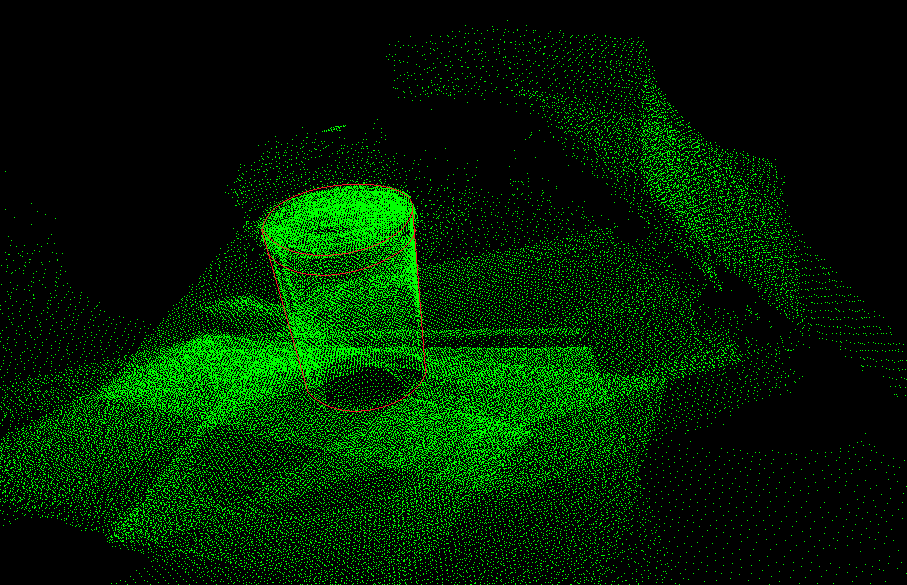
\includegraphics[width=1.0\columnwidth]{pointClouds/bidoneConico.png} 
    \caption{Point Cloud di un bidone Conico}
\end{figure}


\subsection{Primo prototipo}
Il primo protitpo realizzato risponde all'esigenza di catturare e salvare in formato leggibile da un \emph{render} grafico i dati forniti dal sensore di profondità.
Nella sua semplicità ha dato modo allo studente di testare la stabilità delle \emph{API} e produrre della documentazione interna che riportava quali fossero i metodi delle \emph{API} da utlizzare e quali fossero invece quelli poco stabili, sperimentali o addirittura non ancora implementati dal produttore.

\subsection{Secondo prototipo: Cloude}
\subsubsection{Affrontare la discrepanza tra coordinate assolute e coordinate relative}
Un solo \emph{Point Cloud} non è sufficiente a ricostruire un oggetto. Ovviamente il dispositivo, registrando la nuvola di punti inquadrata in un determinato istante, riesce a rilevare solamente i punti che "riesce a vedere": i punti presenti nella parte posteriore dell'oggetto scansionato non possono essere "visti" e conseguentemente nemmeno misurati. Se si vuole avere una ricostruzione completa e non solamente di una facciata è necessario prendere più rilevazioni ed integrarle.\\
Le seuguenti immagini mostrano il \emph{Point Cloud} che descrive la parte anteriore di una scatola rettangolare; dato che la ripresa è stata effettuata da di fronte ed in alto solo le facce superiore ed anteriore sono state memorizzate, mentre delle altre non si hanno dati. I contorni sono stati evidenziati successivamente per permettere una migliore comprensione della forma.
\begin{figure}[!h] 
    \centering 
    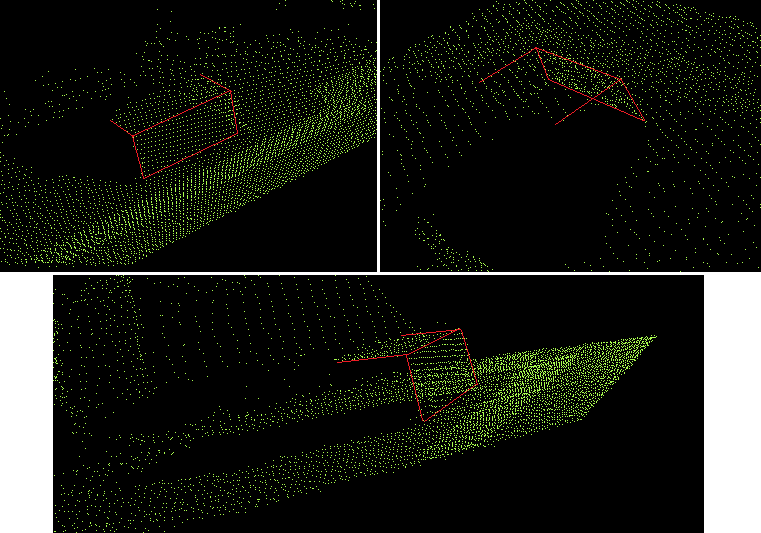
\includegraphics[width=1.0\columnwidth]{pointClouds/singoloShot.png} 
    \caption{Un singolo \emph{Point Cloud}}
\end{figure}
\subsubsection{Approccio}
Questo prototipo, denominato \emph{Cloude}, è stato realizzato allo scopo di rispondere a questa esigenza. L'idea che ne sta a fondamento è la seguente:
\begin{itemize}
	\item Permettere all'utente di scattare alcune foto all'oggetto, quindi di rilevare diversi \emph{Point Cloud}.
	\item Tenere costamente traccia della posizione del dispositivo, in particolare delle posizioni nei momenti in cui vengono scattate le foto.
	\item Usare la posizione relativa al \emph{Point Cloud} per translare e ruotare lo stesso punto a punto, riducendo così le coordinate a dei valori assoluti.
	\item Ora le nuvole di punti registrate sono sovrapponibili le une con le altre e forniscono una prima ricostruzione dell'oggetto.
\end{itemize}

\subsection{Terzo protipo: Samba}
Il prototipo precedente generava delle ricostruzioni riconoscibili, ma piuttosto imprecise.\\
Una analisi dello stesso ha fatto emergere diverse criticità che sono state documentate, assieme alle possibili soluzioni, all'interno di un documento descrittivo. Quest'ultimo è stato alla base dello svilluppo di \emph{Samba}.
\subsubsection{Eccessiva complessità dell'elaborazione}
\emph{Cloude} sfrutta un metedo delle librerie \emph{Tango} che transforma le coordinate di un singolo punto in coordinate assolute fruttando la posizione relativa a cui si trovava il dispositivo, permette di scrivere poco codice, ma ha una elevata complessità. Ciò comporta un sensibile rallentamento dell'elaborazione dei \emph{Point Cloud}. Un \emph{cloud} medio conta intorno ai 90000 punti e con questo approccio richiede mediamente 1,5-2 secondi per essere completamente elaborato, tempo non accettabile per lo scopo per cui l'applicazione è pensata.\\
In \emph{Samba} è stato cambiato radicalmente approccio:
\begin{itemize}
	\item Ad ogni \emph{Point Cloud} viene associata una matrice di transformazione e non la posizione stessa.
	\item In questo modo è sufficiente moltiplicare ogni punto (vettore) per la matrice, che viene calcolata una sola volta per ogni \emph{Poit Cloud}. 
	\item Si è ottenuta così una complessità di \texttt{O(n)} sul numero dei punti da transformare riducendo i tempi di elaborazione da 1,5-2s a circa 200ms (sullo stesso dispositivo).
\end{itemize}
\subsubsection{Bassa qualità delle ricostruzioni}
Nelle ricostruzioni generate da \emph{Cloude} gli oggetti appaiono deformati, spesso i vari \emph{Point Cloud} non si sovrappongono correttamente generando fenomeni di \emph{ghosting}, talvolta rendendo addirittura irriconoscibile l'oggetto.\\
Questo è dovuto ad una scorretta stima della posizione del dispositivo, che induce il calcolo di una erronea matrice di transformazione, e quindi ad un errato posizionamento delle nuvole di punti all'interno dello spazio.\\
Il fenomeno in questione è detto \emph{"drifting"}: i \emph{device Tango}, esattamente come le più comuni applicazioni in realtà aumentata, utilizzano la tecnica del \emph{Motion Tracking} che consiste nel calcolare la propria posizione frequentemente ed in maniera relativa alla coordinate acquisite nella stima precedente. Per quando queste stime siano estremamente precise generano una catena di piccoli errori che sommati tra loro molto presto portano ad una importante discrepanza tra la posizione stimata dal dispositivo e quella reale. Ad esempio partendo da una determinata posizione e camminando in cerchio è praticamente impossibile che la traiettoria stimata passi nuovamente per il punto di partenza.
\begin{figure}[!h] 
    \centering 
    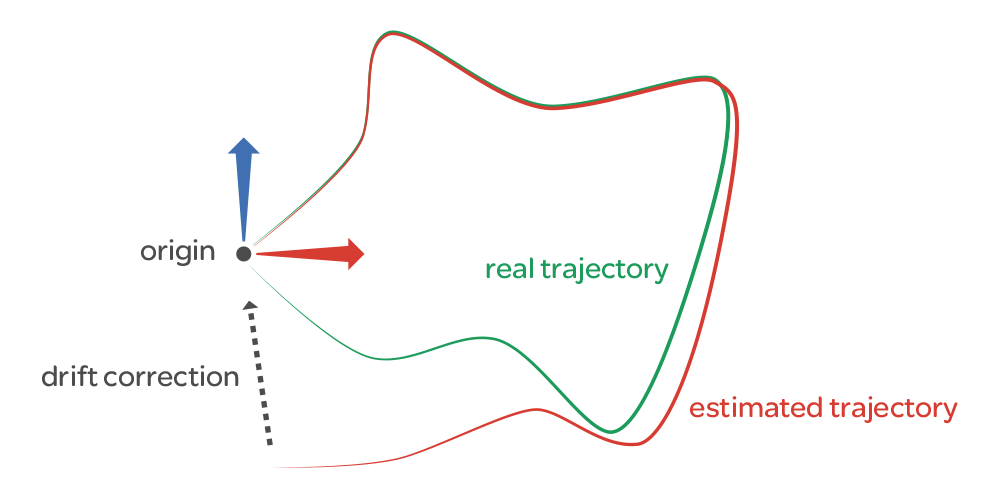
\includegraphics[width=0.9\columnwidth]{varie/Drift_Correction.png} 
    \caption{Motion Tracking}
\end{figure}
Ciò è un limite fisico dei dispositivi, ed è nella pratica impossibile da eliminare, in quanto sarebbe necessario azzerare completamente gli errori relativi.\\
La tecnologua \emph{Tango} però fonrnisce un altro meccanismo di localizzazione: l'\emph{Area Learning}. Le applicazioni ideate per questo tipo di dispositivi infatti hanno la possibilità di mantenere memoria degli spazi che visitano, e successivamente usare queste informazioni per localizzarsi.\\
Il meccanismo è piuttosto simile a quello della memoria spaziale umana: una persona portata bendata all'interno di un edificio sconosciuto, una volta liberata, non avrà alcun mezzo per intuire dove si trovi; se invece la stessa persona fosse condotta all'interno della propria abitazione, alla prima sbirciata noterebbe immediatamente qualche particolare che gli farebbe immediatamente recuperare l'orientamento.\\
Allo stesso modo il tablet è in grado memorizzare alcune \emph{features} all'interno dell'ambiente ed usarle come faro per la triangolazione. \\
Memorizzare completamente un ambiente tuttavia è una operazione che richiede parecchio tempo e costringe l'utente a muoversi per diversi minuti inquadrando tutti i dettagli del luogo dove si trova. Per rendere l'aplicazione maggiornamente responsiva e più vicina alle esigenze dell'utenza \emph{Samba} adotta un approccio detto \emph{Drift Correction}: inzialmente è richiesto all'utente di inquadrare per una ventina di secondi l'ambiente, in maniera da permettere la creazione di una minimale memorizzazione, successivamente il \emph{Motion Tracking} è usato per piccoli spostamenti ma viene corretto nonappena venga inquadrata qualcuna delle (poche) \emph{features} memorizzate. Trasparentemente all'utente, in background, il processo di \emph{Area Learning} continua, memorizzando sempre nuovi dettagli e conseguentemente aumentando sempre più la qualità della registazione.\\

\subsection{Dimensioni eccessive dei file, ridondanza dei punti sovrapposti}
Data la grande mole di punti registrati dai sensori di profondità i \emph{file} contenenti le ricostruzioni generati da \emph{Cloude} sono di dimensione eccessiva, anche più di 10Mb una decina scatti.
Considerando che idealmente gli scatti da riprendere potrebbero essere molti e spesso dovranno essere inviati al \emph{Server} tramite connessione a consumo il peso di questi \emph{file} non è da trascurare.\\
Inoltre c'è una grossa ridondanza di punti: è comune caso d'uso che una stessa zona venga inquadrata in più scatti, quindi tali \emph{Point Cloud} ruotati ed uniti presenterebbero molti punti con le stesse coordinate e semplicemente sovrapposti, qunidi sera dare alcuna informazione aggiuntiva.\\
\emph{Samba} risolve questo problema utilizzando un leggero \emph{voxeling}, ovvero suddividendo lo spazio in cubi o \emph{voxel} di lato prefissato e registrando quali sono i \emph{voxel} che contengono i punti della nuvola.





%**************************************************************
\section{Organizzazione del testo}
xxxx
\begin{description}

    \item[{\hyperref[cap:processi-metodologie]{Il secondo capitolo}}] descrive ...
    
    \item[{\hyperref[cap:descrizione-stage]{Il terzo capitolo}}] approfondisce ...
    
    \item[{\hyperref[cap:analisi-requisiti]{Il quarto capitolo}}] approfondisce ...
    
    \item[{\hyperref[cap:progettazione-codifica]{Il quinto capitolo}}] approfondisce ...
    
    \item[{\hyperref[cap:verifica-validazione]{Il sesto capitolo}}] approfondisce ...
    
    \item[{\hyperref[cap:conclusioni]{Nel settimo capitolo}}] descrive ...
\end{description}

Riguardo la stesura del testo, relativamente al documento sono state adottate le seguenti convenzioni tipografiche:
\begin{itemize}
	\item gli acronimi, le abbreviazioni e i termini ambigui o di uso non comune menzionati vengono definiti nel glossario, situato alla fine del presente documento;
	\item per la prima occorrenza dei termini riportati nel glossario viene utilizzata la seguente nomenclatura: \emph{parola}\glsfirstoccur;
	\item i termini in lingua straniera o facenti parti del gergo tecnico sono evidenziati con il carattere \emph{corsivo}.
\end{itemize}             % Introduzione
% !TEX encoding = UTF-8
% !TEX TS-program = pdflatex
% !TEX root = ../tesi.tex
% !TEX spellcheck = it-IT

%**************************************************************
\chapter{Processi e strumenti}
\label{cap:processi-metodologie}
%**************************************************************

\intro{ xxxx Brevissima introduzione al capitolo}\\

%**************************************************************
\section{Processo sviluppo prodotto}
In ambito aziendale si è scelto di provare, per questo progetto, un processo di sviluppo \emph{software} basato sulla filosofia \emph{Lean}.\\

\subsection{Sviluppo software Lean}
Lo sviluppo \emph{software} \emph{Lean} è caratterizzato da cinque eventi principali, chiamati \emph{milestone} descritti di seguito:\\


\subsubsection{Kick-Off}
Prima riunione ufficiale del team di progetto, momento iniziale del processo di sviluppo; possono partecipare, su invito del \emph{Lean Project Leader}, anche persone che non fanno parte del team di progetto ma che sono portatori di interessi verso l’iniziativa da sviluppare. Coincide con l’inizio della fase di \textbf{allestimento} e \textbf{avviamento} in cui viene determinata la natura e lo scopo del progetto.\\

\subsubsection{Concept Preview}
Momento in cui è disponibile un primo campione (\emph{concept}, \emph{hardware} e/o \emph{software}) del nuovo prodotto. Il \emph{concept} può essere incompleto e affetto da errori. Rappresenta il concetto principale che andrà a costituire il nuovo prodotto (es. dimensioni, user interface, usabilità). Il \emph{concept} è oggetto di riesame, con lo scopo di valutare se lo sviluppo della progettazione è in linea con gli obiettivi definiti dalla \emph{Value Proposition}. Condizione necessaria al raggiungimento della \emph{milestone} è avere eseguito tale riesame con esito positivo. Coincide con l’inizio della fase di sviluppo della progettazione fino al livello di dettaglio ritenuto opportuno e necessario per l’esecuzione del progetto.\\

\subsubsection{Product Prototype}
Momento in cui è disponibile il primo prototipo del nuovo prodotto, completo nelle sue funzioni (sviluppo finito) ma non ancora messo a punto mediante verifiche e correzioni, per garantirne funzionalità e prestazioni. Può essere dato in valutazione a clienti interni o a partner strategici. Condizione necessaria al raggiungimento della \emph{milestone} è aver eseguito un riesame generale della progettazione prima della realizzazione dei prototipi, con lo scopo di valutare se lo sviluppo della progettazione è in linea con gli obiettivi definiti dalla \emph{Value Proposition} e della \emph{Requirements Specification}. Coincide con il termine della fase di progettazione e l’inizio della fase di esecuzione, cioè l’insieme dei processi necessari a soddisfare i requisiti del progetto.\\

\subsubsection{Product Design Freeze}
Momento in cui viene definitivamente congelata la progettazione
del nuovo prodotto; non sono più ammesse modifiche o aggiunte ai requisiti
di prodotto: la \emph{R.S.} è completa e definitiva. I campioni prodotti possono essere
dati in valutazione anche ai clienti finali. Il progetto del nuovo prodotto è stato
verificato e validato, il processo produttivo è stato completamente definito ma non
ancora validato. Condizione necessaria al raggiungimento della \emph{milestone} è aver
eseguito un riesame generale della progettazione prima dell’implementazione delle
modifiche da apportare al prodotto e alle attrezzature di produzione, conseguenti
la fase di verifica, con lo scopo di valutare se lo sviluppo della progettazione è in
linea con gli obiettivi definiti dalla \emph{Value Proposition} e della \emph{R.S.}. Coincide il
termine della fase di esecuzione e l’inizio della fase di monitoraggio e controllo.
Tale fase è formata dai processi attuati per osservare e misurare l’esecuzione del
progetto in modo da identificarne per tempo i rischi e i potenziali problemi e intraprendere,
quando necessarie, le azioni correttive volte a rimettere il progetto
in linea con i propri obiettivi.\\

\subsubsection{Start Of Production (SOP)}
Momento a partire dal quale la produzione in serie
del nuovo prodotto può iniziare; durante le pre-serie il prodotto realizzato dalla
linea produttiva è stato verificato e validato e il processo produttivo e logistico è
stato messo a punto, verificato e validato; i codici del nuovo prodotto sono stati
attivati; il piano di lancio è stato definito e comunicato. Le \emph{Lesson Learned} sono
state prodotte e condivise con i colleghi del Centro di Competenza. Coincide con la fase di completamento. Tale fase prevede l’accettazione formale del prodotto
e l’esecuzione di tutte le attività documentali indirizzate a chiudere tutte
le pendenze, inclusa l’archiviazione dei documenti e la redazione dei rapporti di
chiusura.\\


\subsection{Applicazione}
Dato che il progetto di \emph{stage} ha durata temporale limitata è stato imposto come obiettivo quello di raggiungere solo la \emph{milestone} denominata \emph{Product Prototype}. Le fasi successive potranno essere svolte in futuro nel caso in cui l'azienda ritenga opportuno proseguire con il progetto.


\section{Strumenti}
L'azienda ha lasciato grande libertà riguardo agli strumenti da utilizzare per questo progetto, quindi essi sono stati fissati inizialmente e successivamente incrementati al crescere delle necessità.

\subsection{Codice}
Segue la lista degli strumenti utilizzati per la codifica.
\begin{itemize}
	\item \textbf{Java}: Il linguaggio preferito per l'applicazione lato \emph{tablet}. È stato scelto seguendo le \emph{Best Practice} dello sviluppo \emph{Android}.
	\item \textbf{C++}: Il linguaggio preferito per l'applicazione lato \emph{Server}. È stato scelto perché tutti le più diffuse librerie per l'elaborazione dei \emph{Point Cloud} sono disponibili in questo linguaggio.
	\item \textbf{PCD, Point Cloud Library}: Una delle librerie di maggior rilievo nel campo della \emph{Computer Vision}, mette a disposizione innumerevoli funzionalità per elaborazione ed ottimizzazione dei \emph{Point Cloud}.
	\item \textbf{Tango API}: Le \emph{API} ufficiali per lo sviluppo di applicazioni \emph{Tango}.
	\item \textbf{PHP}: Il linguaggio usato per ricevere ed inviare le richieste \emph{http} quando si necessita comunicazione tra \emph{Server} e dispositivo.
\end{itemize}

\subsection{IDE ed editor}
Segue la lista degli embienti per la codifica utilizzati durante il progetto.
\begin{itemize}
	\item \textbf{Android Studio}: L'\emph{IDE} ufficiale per le applicazioni \emph{Android}.
	\item \textbf{QT}: L'\emph{IDE} scelto per lo sviluppo del codice \emph{C++}.
	\item \textbf{Sublime Text 2}: L'\emph{editor} di testo usato per scrivere gli \emph{script} \emph{php}.
\end{itemize}

\subsection{Framework}
Segue la lista dei \emph{Framework} usati per il 












             % Processi
% !TEX encoding = UTF-8
% !TEX TS-program = pdflatex
% !TEX root = ../tesi.tex
% !TEX spellcheck = it-IT

%**************************************************************
\chapter{Descrizione dello stage}
\label{cap:descrizione-stage}
%**************************************************************

\intro{xxxx Breve introduzione al capitolo}\\

%**************************************************************
\section{Introduzione al progetto}
Data la natura innovativa del progetto è stato necessario 

%**************************************************************
\section{Analisi preventiva dei rischi}

Durante la fase di analisi iniziale sono stati individuati alcuni possibili rischi a cui si potrà andare incontro.
Si è quindi proceduto a elaborare delle possibili soluzioni per far fronte a tali rischi.\\

\begin{risk}{Performance del simulatore hardware}
    \riskdescription{le performance del simulatore hardware e la comunicazione con questo potrebbero risultare lenti o non abbastanza buoni da causare il fallimento dei test}
    \risksolution{coinvolgimento del responsabile a capo del progetto relativo il simulatore hardware}
    \label{risk:hardware-simulator} 
\end{risk}

%**************************************************************
\section{Requisiti e obiettivi}


%**************************************************************
\section{Pianificazione}             % Kick-Off
% !TEX encoding = UTF-8
% !TEX TS-program = pdflatex
% !TEX root = ../tesi.tex
% !TEX spellcheck = it-IT
%**************************************************************
\chapter{Analisi dei requisiti}
\label{cap:analisi-requisiti}
%**************************************************************

\intro{Un progetto software innovativo pone il progettista dinanzi a molti canti di Sirena che rischiano di indurlo ad investire risorse per scopi futili. Per questo l'Analisi dei Requisiti è stata stilata nelle prime fasi del processo e poi seguita il più scrupolosamente possibile.}\\

\section{Casi d'uso}

Per lo studio dei casi d'uso del prodotto sono stati realizzati dei diagrammi.
I diagrammi dei casi d'uso (in inglese \emph{Use Case Diagram}) sono diagrammi di tipo \gls{uml} dedicati alla descrizione delle funzioni o servizi offerti da un sistema, così come sono percepiti e utilizzati dagli attori che interagiscono col sistema stesso.
Per ogni \emph{use case} sono stati inoltre riportati:
\begin{itemize}
	\item Attori Principali
	\item Precondizioni
	\item Descrizione/flusso degli eventi
	\item Postcondizioni
\end{itemize}
Seguono i diagrammi riguardanti l'applicativo lato \emph{tablet}, ovvero quello di cui lo studente si è occupato di persona.


\subsection{UC0: Scenario principale}
\begin{figure}[H] 
    \centering 
    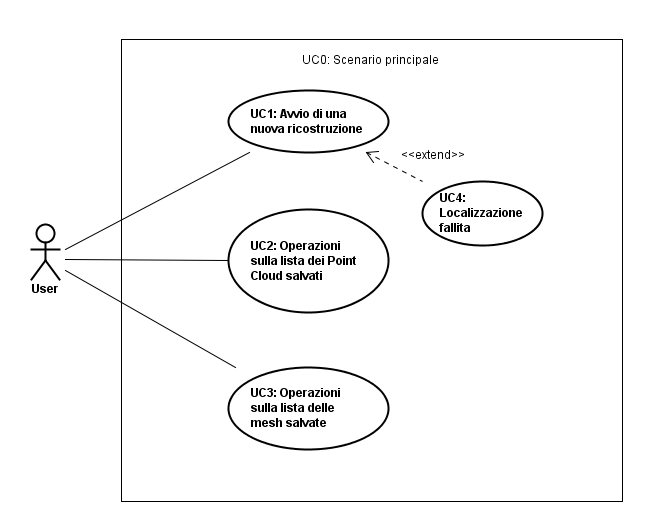
\includegraphics[width=0.9\columnwidth]{usecase/UC0.png} 
    \caption{Use Case - UC0: Scenario principale}
\end{figure}
\ \\
\textbf{Attori Principali}: Utente.
\\\\ \textbf{Precondizioni}: L'utente ha avviato l'applicazione su un dispositivo \emph{Tango} ed ha fornito tutti i permessi necessari, ovvero:
\begin{itemize}
	\item Area Learning (permesso speciale per dispositivi \emph{Tango}).
	\item Lettura e scrittura su disco.
	\item Utilizzo fotocamera.
	\item Accesso ad internet.
\end{itemize}
Inoltre deve aver avviato l'applicazione in un ambiente sufficientemente illuminato.
\\\\ \textbf{Descrizione}: La schermata principale, mentre è immediatamente in atto il processo di localizzazione, mette a disposizione il \emph{render} dei punti e tutti gli strumenti per permettere all'utente di effettuare la rilevazione e di accedere agli altri menù.
\\\\ \textbf{Postcondizioni}: Il sistema è pronto per permettere una nuova interazione con l'utente.


\subsection{UC1: Avvio di una nuova ricostruzione}
\begin{figure}[H] 
    \centering 
    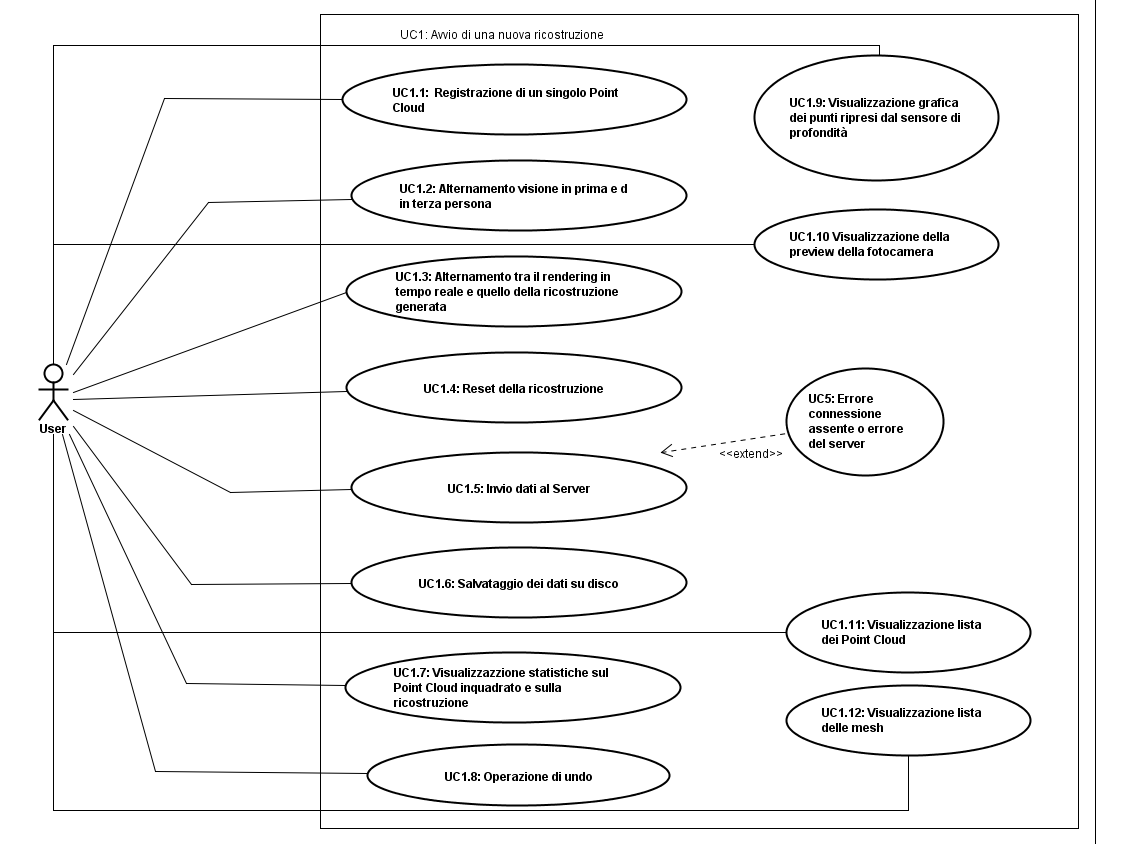
\includegraphics[width=1.0\columnwidth]{usecase/UC1.png} 
    \caption{Use Case - UC1: Avvio di una nuova ricostruzione}
\end{figure}
\ \\
\textbf{Attori Principali}: Utente.
\\\\ \textbf{Precondizioni}: L'utente ha aperto l'applicazione ed è rimasto in attesa della localizzazione nella schermata principale.
\\\\ \textbf{Descrizione}: L'utente ha a disposizione tutti gli strumenti per registrare, controllare e perfezionare la ricostruzione dell'oggetto da ispezionare. Inoltre gli sono forniti i tasti per passare alle altre funzionalità. 
\\\\ \textbf{Postcondizioni}: L'utente ha terminato una registrazione inviandola al \emph{Server}, salvandola su disco, oppure scartandola.



\subsection{UC1.1: Registrazione di un singolo Point Cloud}
\textbf{Attori Principali}: Utente.
\\\\ \textbf{Precondizioni}:  L'utente ha aperto l'applicazione, è rimasto in attesa della localizzazione nella schermata principale ed intende registrare un nuovo scatto.
\\\\ \textbf{Descrizione}: L'utente inquadra il soggetto della rilevazione e preme il tasto "Shot".
\\\\ \textbf{Postcondizioni}: Il sistema ha catturato il \emph{Point Cloud} inquadrato e l'ha aggiunto alla ricostruzione attualmente in corso.

\subsection{UC1.2: Alternanza visione in prima ed in terza persona}
\textbf{Attori Principali}: Utente.
\\\\ \textbf{Precondizioni}: L'utente ha aperto l'applicazione, è rimasto in attesa della localizzazione nella schermata principale e sta osservando il \emph{render}.
\\\\ \textbf{Descrizione}: L'utente, usando i tasti "First" o "Third" alterna tra la visuale in prima ed in terza persona per il \emph{render}.
\\\\ \textbf{Postcondizioni}: Il \emph{render} mostra sullo schermo i suoi contenuti nella modalità scelta dall'utente.

\subsection{UC1.3: Alternanza tra il rendering in tempo reale e quello della ricostruzione generata}
\textbf{Attori Principali}: Utente.
\\\\ \textbf{Precondizioni}: L'utente ha aperto l'applicazione, è rimasto in attesa della localizzazione nella schermata principale ed ha già iniziato la rilevazione, avendo quindi salvato in memoria almeno un Point Cloud singolo.
\\\\ \textbf{Descrizione}: L'utente, usando l'interruttore denominato "Reconstrucion Mode", alterna tra la visualizzazione dei punti attualmente catturati dal sensore di profondità e quella della ricostruzione in corso.
\\\\ \textbf{Postcondizioni}: Il \emph{render} mostra sullo schermo i contenuti selezionati dall'utente.

\subsection{UC1.4: Reset della ricostruzione}
\textbf{Attori Principali}: Utente.
\\\\ \textbf{Precondizioni}: L'utente ha aperto l'applicazione, è rimasto in attesa della localizzazione nella schermata principale ed ha intenzione di scartare interamente la rilevazione effettuata fino a quel momento.
\\\\ \textbf{Descrizione}: L'utente premendo sul pulsante "Reset" azzera i punti salvati e rende il dispositivo pronto per una nuova rilevazione.
\\\\ \textbf{Postcondizioni}: Il dispositivo non ha più alcuna ricostruzione in corso ed è pronto ad iniziarne una nuova.

\subsection{UC1.5: Invio dati al Server}
\textbf{Attori Principali}: Utente.
\\\\ \textbf{Precondizioni}: L'utente ha aperto l'applicazione, è rimasto in attesa della localizzazione nella schermata principale, ha effettuato una rilevazione che lo soddisfa ed intende inviarla al \emph{Server}.
\\\\ \textbf{Descrizione}: L'utente premendo sul pulsante "Send Data To Server" invia la ricostruzione corrente al \emph{Server} in formato \texttt{pcd}.
\\\\ \textbf{Postcondizioni}: La ricostruzione corrente è stata inviata al \emph{Server}, ma non eliminata dalla memoria. Sarà quindi possibile continuare la rilevazione.

\subsection{UC1.6: Salvataggio dei dati su disco}
\textbf{Attori Principali}: Utente.
\\\\ \textbf{Precondizioni}: L'utente ha aperto l'applicazione, è rimasto in attesa della localizzazione nella schermata principale, ha effettuato una rilevazione che lo soddisfa ed intende salvarla su disco.
\\\\ \textbf{Descrizione}: L'utente, premendo sul pulsante "Save" ed inserendo un nome per il \emph{file}, salva la ricostruzione corrente su disco in formato \texttt{pcd}.
\\\\ \textbf{Postcondizioni}: La ricostruzione corrente è stata salvata su disco, ma non eliminata dalla memoria. Sarà quindi possibile continuare la rilevazione.

\subsection{UC1.7: Visualizzazione statistiche}
\textbf{Attori Principali}: Utente.
\\\\ \textbf{Precondizioni}: L'utente ha aperto l'applicazione, è rimasto in attesa della localizzazione nella schermata principale.
\\\\ \textbf{Descrizione}: L'utente può consultare le statistiche riguardanti il \emph{Point Cloud} inquadrato e la ricostruzione nell'angolo in alto a sinistra dello schermo. Tali statistiche sono:
\begin{itemize}
	\item Numero dei punti attualmente inquadrati.
	\item Distanza media dei punti attualmente inquadrati.
	\item Numero degli scatti presi fino a quel momento.
	\item Numero di punti presenti nella ricostruzione fino a quel momento.
	\item \emph{Frame Of Reference} e \emph{Status} della rilevazione.
	\item Posizione $x$, $y$ e $z$ del dispositivo.
\end{itemize} 
\ \\ \textbf{Postcondizioni}: L'utente ha visualizzato le statistiche.

\subsection{UC1.8: Operazione di undo}
\textbf{Attori Principali}: Utente.
\\\\ \textbf{Precondizioni}: L'utente ha aperto l'applicazione, è rimasto in attesa della localizzazione nella schermata principale, ha effettuato uno o più \emph{shot} che ritiene errati o di bassa qualità ed intende scartarli.
\\\\ \textbf{Descrizione}: L'utente, premendo sul pulsante "Undo", scarta l'ultimo \emph{Point Cloud} registrato.
\\\\ \textbf{Postcondizioni}: L'ultimo \emph{Point Cloud} registrato viene scartato.




\subsection{UC2: Operazioni sulla lista dei Point Cloud salvati}
\begin{figure}[H] 
    \centering 
    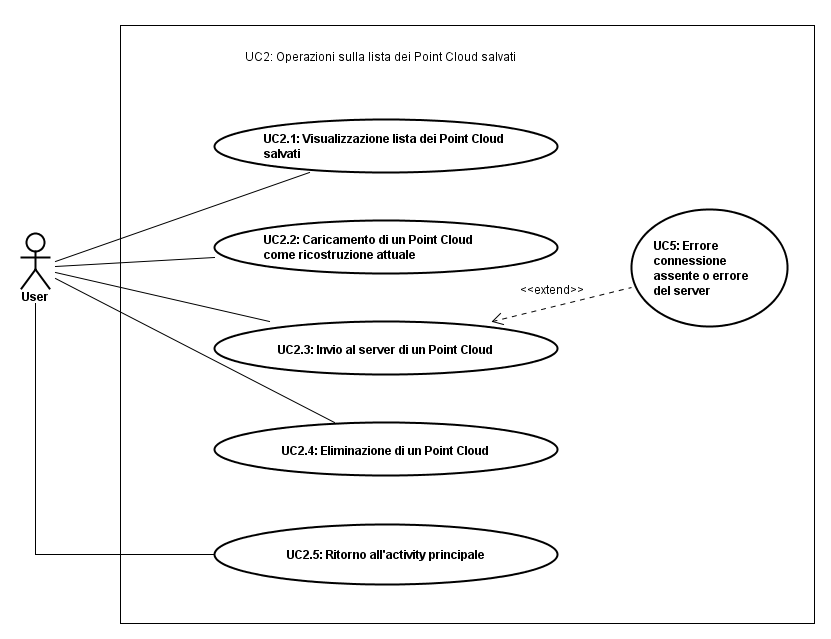
\includegraphics[width=0.9\columnwidth]{usecase/UC2.png} 
    \caption{Use Case - UC2: Operazioni sulla lista dei Point Cloud salvati}
\end{figure}
\ \\
\textbf{Attori Principali}: Utente.
\\\\ \textbf{Precondizioni}: L'utente ha aperto l'applicazione ed ha premuto sul pulsante per visualizzare la lista delle ricostruzioni 3D salvate su disco.
\\\\ \textbf{Descrizione}: L'utente vede sullo schermo la lista delle ricostruzioni 3D salvate su disco su cui può effettuare diverse azioni.
\\\\ \textbf{Postcondizioni}: Il sistema è pronto per ricevere una nuova interazione.


\subsection{UC2.1: Visualizzazione lista dei PointCloud salvati}
\textbf{Attori Principali}: Utente.
\\\\ \textbf{Precondizioni}: L'utente ha aperto l'applicazione, ha premuto sul pulsante per visualizzare la lista delle ricostruzioni 3D salvate su disco.
\\\\ \textbf{Descrizione}: L'utente consulta la lista dei \emph{Point Cloud} salvati su disco.
\\\\ \textbf{Postcondizioni}: Nessuna.

\subsection{UC2.2: Caricamento di un Point Cloud come ricostruzione attuale}
\textbf{Attori Principali}: Utente.
\\\\ \textbf{Precondizioni}: L'utente ha aperto l'applicazione, ha premuto sul pulsante per visualizzare la lista delle ricostruzioni 3D salvate su disco ed intende caricare una di queste come ricostruzione attuale.
\\\\ \textbf{Descrizione}: L'utente, premendo sul nome del \emph{file} scelto, lo carica come ricostruzione corrente.
\\\\ \textbf{Postcondizioni}: Il sistema ritorna all'\emph{activity} principale (quella degli UC1.*) con la ricostruzione caricata da file come ricostruzione corrente.

\subsection{UC2.3: Invio al Server di un Point Cloud}
\textbf{Attori Principali}: Utente.
\\\\ \textbf{Precondizioni}: L'utente ha aperto l'applicazione, ha premuto sul pulsante per visualizzare la lista delle ricostruzioni 3D salvate su disco ed ha intenzione di inviare al server uno dei \emph{Point Cloud} salvati.
\\\\ \textbf{Descrizione}: L'utente applica una lunga pressione sul nome del \emph{file} scelto, apparirà un menù; da quest'ultimo l'utente seleziona "Send To Server" e la ricostruzione sarà mandata al \emph{Server} in formato \texttt{pcd}. Generalmente questa funzione viene sfruttata se quando si effettua una rilevazione non si ha immediatamente la possibilità di inviare i dati tramite \emph{Internet}.
\\\\ \textbf{Postcondizioni}: Il \emph{File} selezionato viene correttamente spedito al \emph{Server}.

\subsection{UC2.4: Eliminazione di un Point Cloud}
\textbf{Attori Principali}: Utente.
\\\\ \textbf{Precondizioni}: L'utente ha aperto l'applicazione, ha premuto sul pulsante per visualizzare la lista delle ricostruzioni 3D salvate su disco ed ha intenzione di cancellare uno dei \emph{File} salvati.
\\\\ \textbf{Descrizione}: L'utente applica una lunga pressione sul nome del \emph{file} scelto, apparirà un menù; da quest'ultimo l'utente seleziona "Delete" ed il \emph{File} selezionato viene cancellato.
\\\\ \textbf{Postcondizioni}: Il \emph{File} selezionato è stato cancellato e non è più presente su disco.

\subsection{UC2.5: Ritorno all'activity principale}
\textbf{Attori Principali}: Utente.
\\\\ \textbf{Precondizioni}: L'utente ha aperto l'applicazione, ha premuto sul pulsante per visualizzare la lista delle ricostruzioni 3D salvate su disco ma desidera ritornare all'\emph{activity} principale.
\\\\ \textbf{Descrizione}: L'utente preme sul tasto "Back" e ritorna all'\emph{activity} principale.
\\\\ \textbf{Postcondizioni}: L'utente ritorna all'\emph{activity} principale.


\subsection{UC3: Operazioni sulla lista delle mesh salvate}
\begin{figure}[H] 
    \centering 
    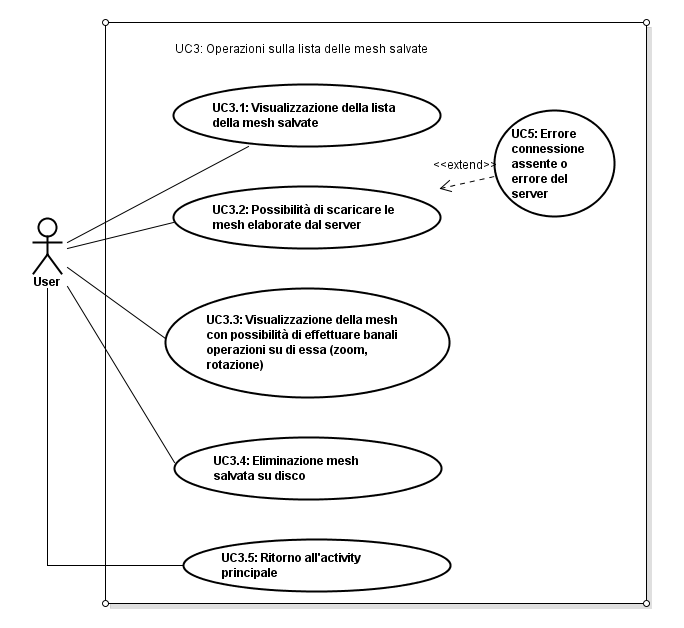
\includegraphics[width=0.9\columnwidth]{usecase/UC3.png} 
    \caption{Use Case - UC3: Operazioni sulla lista delle mesh salvate}
\end{figure}
\ \\
\textbf{Attori Principali}: Utente.
\\\\ \textbf{Precondizioni}: L'utente ha aperto l'applicazione ed ha premuto sul pulsante per visualizzare la lista delle \emph{mesh} salvate su disco.
\\\\ \textbf{Descrizione}: L'utente vede sullo schermo la lista \emph{mesh} salvate su disco su cui può effettuare diverse azioni.
\\\\ \textbf{Postcondizioni}: Il sistema è pronto per ricevere una nuova interazione.




\subsection{UC3.1: Visualizzazione della lista delle mesh salvate}
\textbf{Attori Principali}: Utente.
\\\\ \textbf{Precondizioni}: L'utente ha aperto l'applicazione ed ha premuto sul pulsante per visualizzare la lista delle \emph{mesh} salvate su disco.
\\\\ \textbf{Descrizione}:  L'utente consulta la lista delle \emph{mesh} salvate su disco.
\\\\ \textbf{Postcondizioni}: Nessuna.

\subsection{UC3.2: Possibilità di scaricare le mesh elaborate dal Server}
\textbf{Attori Principali}: Utente.
\\\\ \textbf{Precondizioni}: L'utente ha aperto l'applicazione, ha premuto sul pulsante per visualizzare la lista delle \emph{mesh} salvate su disco ed ha intenzione di aggiornare la lista di \emph{mesh} aggiungendo le altre presenti sul \emph{Server}.
\\\\ \textbf{Descrizione}: L'utente preme sul simbolo di \emph{refresh} in alto a destra e ricarica la lista di \emph{mesh} eventualmente scaricando quelle sul \emph{Server} ma non sul dispositivo.
\\\\ \textbf{Postcondizioni}: L'utente ha a disposizione una lista aggiornata di \emph{mesh}.

\subsection{UC3.3: Visualizzazione grafica delle mesh}
\textbf{Attori Principali}: Utente.
\\\\ \textbf{Precondizioni}: L'utente ha aperto l'applicazione, ha premuto sul pulsante per visualizzare la lista delle \emph{mesh} salvate su disco ed intende visualizzare una specifica \emph{mesh} in 3D.
\\\\ \textbf{Descrizione}: L'utente preme sul nome della \emph{mesh} che intende visualizzare, a questo punto si apre un piccolo ambiente grafico 3D dove l'utente può osservare la ricostruzione ed effettuare banali operazioni su di essa.
\\\\ \textbf{Postcondizioni}: Nessuna.

\subsection{UC3.4: Eliminazione mesh salvata su disco}
\textbf{Attori Principali}: Utente.
\\\\ \textbf{Precondizioni}: L'utente ha aperto l'applicazione, ha premuto sul pulsante per visualizzare la lista delle \emph{mesh} salvate su disco.
\\\\ \textbf{Descrizione}: L'utente effettuerà le operazioni necessarie per cancellare la \emph{mesh}.
\\\\ \textbf{Postcondizioni}: Il \emph{File} selezionato è stato cancellato e non è più presente su disco.

\subsection{UC3.5: Ritorno all'activity principale}
\textbf{Attori Principali}: Utente.
\\\\ \textbf{Precondizioni}: L'utente ha aperto l'applicazione, ha premuto sul pulsante per visualizzare la lista delle \emph{mesh} salvate su disco ma desidera ritornare all'\emph{activity} principale.
\\\\ \textbf{Descrizione}: L'utente preme sul tasto "Back" e ritorna all'\emph{activity} principale.
\\\\ \textbf{Postcondizioni}: L'utente ritorna all'\emph{activity} principale.


\subsection{UC4: Localizzazione fallita}
\textbf{Attori Principali}: Utente.
\\\\ \textbf{Precondizioni}: Le operazioni di localizzazione non sono andate a buon fine.
\\\\ \textbf{Descrizione}: L'utente non sarà in grado di procedere alla rilevazione, sarà mostrato un messaggio d'errore.
\\\\ \textbf{Postcondizioni}: Non può essere effettuata alcuna rilevazione.


\subsection{UC5: Errore connessione assente o errore del Server}
\textbf{Attori Principali}: Utente.
\\\\ \textbf{Precondizioni}: L'utente cerca di compiere una operazione che richieda comunicazione con il \emph{Server} senza disporre di una connessione ad internet.
\\\\ \textbf{Descrizione}: L'utente sarà avvisato del fallimento dell'operazione ma potrà ritentare in seguito.
\\\\ \textbf{Postcondizioni}: La comunicazione tra dispositivo e \emph{Server} non va a buon fine.



\section{Requisiti}

Da un'attenta analisi dei requisiti e degli use case effettuata sul progetto è stata stilata la tabella che traccia i requisiti in rapporto agli use case.\\
Sono stati individuati diversi tipi di requisiti e si è quindi fatto utilizzo di un codice identificativo per distinguerli.\\
Il codice dei requisiti è così strutturato R [F\text{\textbar}Q\text{\textbar}V\text{\textbar}P] [D\text{\textbar}O] dove:
\begin{enumerate}
	\item[R =] requisito
	
    \item[F =] funzionale
    \item[Q =] qualitativo
    \item[V =] di vincolo
    \item[P =] prestazionale
    
    \item[O =] obbligatorio
    \item[D =] desiderabile
\end{enumerate}
Nelle tabelle seguenti sono riassunti i requisiti e il loro tracciamento con gli \emph{use case} delineati in fase di analisi.

\subsection{Requisiti Funzionali}
\LTXtable{\textwidth}{tabelle/requisiti/funzionali.tex}


\subsection{Requisiti Qualitativi}
\LTXtable{\textwidth}{tabelle/requisiti/qualitativi.tex}

\subsection{Requisiti di Vincolo}
\LTXtable{\textwidth}{tabelle/requisiti/vincolo.tex}

\subsection{Requisiti Prestazionali}
\LTXtable{\textwidth}{tabelle/requisiti/prestazionali.tex}

















             % Concept Preview
% !TEX encoding = UTF-8
% !TEX TS-program = pdflatex
% !TEX root = ../tesi.tex
% !TEX spellcheck = it-IT

%**************************************************************
\chapter{Progettazione e codifica}
\label{cap:progettazione-codifica}
%**************************************************************

\intro{In questo capitolo verrà descritta la progettazione dell'ultimo prototipo prodotto.}\\


\section{Metodo e formalismo di specifica}
Nell'esposizione dell'architettura del prodotto si procederà con un approccio di tipo top-down.  Si descriverà quindi l'architettura iniziando dal generale ed andando al particolare; descrivendo prima i componenti, per poi descrivere nel dettaglio le singole classi.\\
Per ogni componente saranno descritti brevemente il tipo, l'obiettivo e la funzione e saranno specificati
eventuali figli, classi ed interazioni con altri componenti. Ogni classe sarà dotata di una breve descrizione e
ne saranno specificate le responsabilità, le classi ereditate, le sottoclassi e le relazioni con altre classi.\\
Infine si illustreranno degli esempi di utilizzo dei \emph{design pattern} nell'architettura del sistema.

\section{Legenda}
Tutti i diagrammi usano la convenzione di colori descritta nella legenda in figura~\ref{fig:legenda} al fine di migliorare la leggibilità. I livelli di annidamento sono da intendere per la totale struttura dei package e non solo per il singolo schema.\\
Si noti in particolare che le classi e componenti di colore arancio rappresentano classi di librerie esterne al sistema, ma vengono talora rappresentate comunque per maggiore chiarezza.
\begin{figure}[H] 
    \centering 
    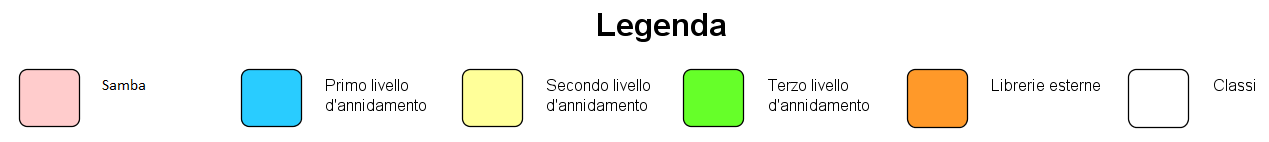
\includegraphics[width=1.0\columnwidth]{varie/Legenda.png} 
    \caption{Legenda}\label{fig:legenda}
\end{figure}


\section{Architettura generale}
L'architettura generale è di tipo \emph{Client-Server}, la comunicazione avviene tramite semplici richieste \emph{http} e alcune notifiche vengono inviate tramite \emph{FireBase}.\\
Questo documento tuttavia esporrà solamente la parte di progettazione riguardante l'applicativo lato \emph{client}.\\
L'architettura generale della applicazione \emph{Android} è di tipo \emph{MVP} ovvero \emph{Model View Presenter}. Questo genere di architettura è stato scelto alla luce delle \emph{Android Best Practices}.\\
Il \emph{Model} contiene tutta la \emph{business logic} dell'applicazione.\\
Il \emph{Presenter} si occupa sia di osservare il modello che di aggiornare/osservare la vista. Nel caso specifico il \emph{Presenter} è composto dall'insieme delle \emph{activity} necessarie al sistema.\\
La \emph{View} è composta da \emph{file} \emph{xml} che rappresentano \emph{template} di visualizzazione e sono completamente passivi. Per questo non verranno trattati nella sezione \ref{cap:componenti-classi}.\\
Il diagramma in figura \ref{fig:arc_generale} rappresenta informalmente la struttura generale del sistema e non rispecchia la reale nomenclatura e struttura del \emph{package}.
\begin{figure}[H] 
    \centering 
    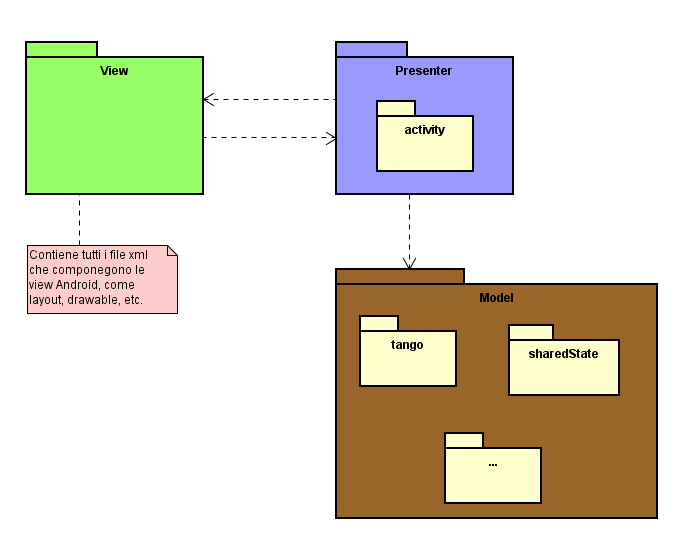
\includegraphics[width=0.9\columnwidth]{st/arc_gen_MVP.png} 
    \caption{Architettura generale del sistema}\label{fig:arc_generale}
\end{figure}



%**************************************************************
\section{Componenti e classi}\label{cap:componenti-classi}
La volontà di realizzare un prototipo ha avuto molto peso anche nella fase di progettazione. Per questo semplicità e rapidità di sviluppo sono stati obiettivi prioritari, anche sacrificando parzialmente riuso e testabilità. Ciò è stato ritenuto accettabile in quanto il prodotto non ha lo scopo di essere incrementato fino a divenire un prodotto finito, ma solo quello di essere premessa sperimentale/prototipale per un progetto futuro.\\
Di seguito viene riportata la lista delle componenti del sistema.

\subsection{Samba}
\begin{figure}[H] 
    \centering 
    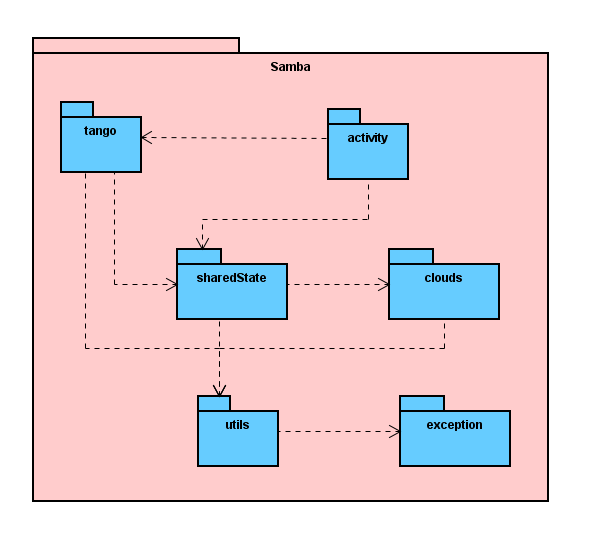
\includegraphics[width=0.9\columnwidth]{st/Samba.png} 
    \caption{Componente Samba}\label{fig:comp-Samba}
\end{figure}
\subsubsection{Descrizione}
È il livello principale del sistema lato \emph{tablet}.
\subsubsection{Package figli}
\begin{itemize}
	\item Samba.activity
	\item Samba.tango
	\item Samba.sharedState
	\item Samba.clouds
	\item Samba.utils
	\item Samba.exception
\end{itemize}

\subsection{Samba.activity}
\begin{figure}[H] 
    \centering 
    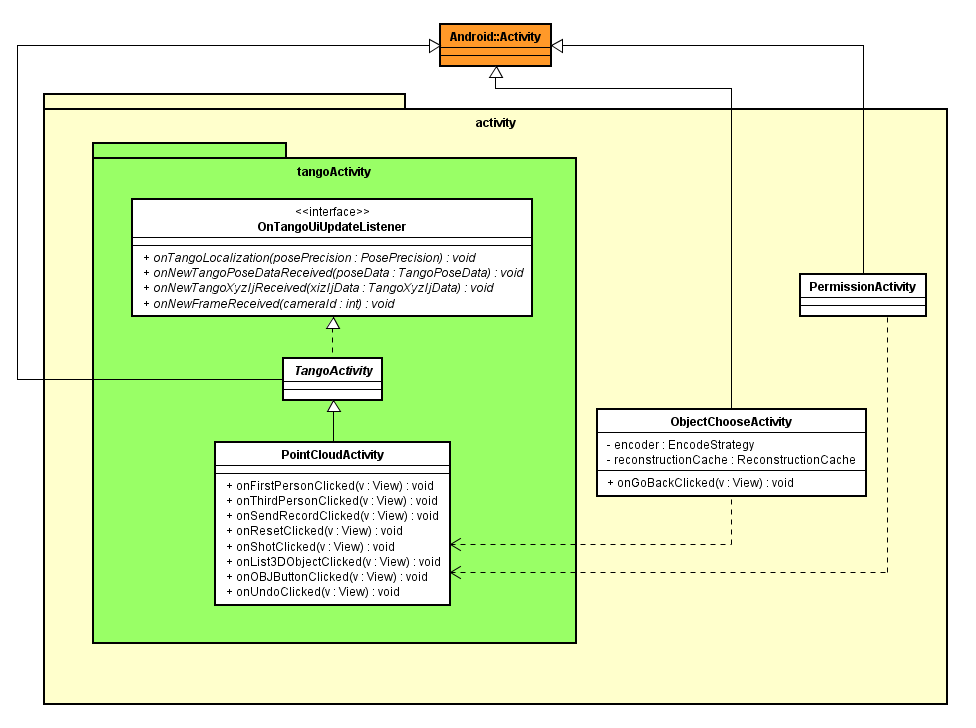
\includegraphics[width=1.0\columnwidth]{st/Samba_activity.png} 
    \caption{Componente Samba.activity}
\end{figure}
\subsubsection{Descrizione}
Questo \emph{package} contiene tutte le \emph{activity} necessarie per l'applicazione. Contiene inoltre la definizione di una interfaccia per le attività che vogliono fare uso dei vari \emph{manager} messi a disposizione (si veda sezione \ref{subs:samba-tango}).
\subsubsection{Package figli}
\begin{itemize}
	\item Samba.activity.tangoActivity
\end{itemize}
\subsubsection{Classi}
\begin{itemize}
	\item Samba.activity.PermissionActivity
	\item Samba.activity.ObjectChooseActivity
\end{itemize}

\subsection{Samba.activity.tangoActivity}
\subsubsection{Descrizione}
Questo \emph{package} serve a contenere tutte le \emph{activity} che vogliono essere attività Tango, ovvero che vogliono poter usare i \emph{manager} messi a disposizione (si veda sezione \ref{subs:samba-tango}).
\subsubsection{Interfacce}
\begin{itemize}
	\item Samba.activity.tangoActivity.OnTangoUiUpdateListener
\end{itemize}
\subsubsection{Classi}
\begin{itemize}
	\item Samba.activity.tangoActivity.TangoActivity
	\item Samba.activity.tangoActivity.PointCloudActivity
\end{itemize}

\subsection{Samba.activity.tangoActivity.OnTangoUiUpdateListener}
\subsubsection{Descrizione}
Interfaccia che deve essere implementata da tutte le \emph{activity} che vogliono fare uso dei \emph{manager Tango} messi a disposizione (si veda sezione \ref{subs:samba-tango}). Espone metodi pubblici che possono essere chiamati da altre componenti quando avranno la necessità di notificare qualche cambiamento di stato.
\subsubsection{Utilizzo}
Viene implementate dalle \emph{activity} che vogliono interagire con il ciclo di vita dei sensori \emph{Tango}. Verrà usata per permettere indirettamente alle componenti che gestiscono i sensori \emph{Tango} di aggiornare la \emph{UI}.
\subsubsection{Implementata da}
\begin{itemize}
	\item Samba.activity.tangoActivity.TangoActivity
\end{itemize}
\subsubsection{Relazioni con altre classi}
\begin{itemize}
 \item \texttt{Samba.clouds.utils.poseSanity.PosePrecision}: relazione uscente, dipendenza, utilizzo come parametro di uno o più metodi.
\end{itemize}

\subsection{Samba.activity.tangoActivity.TangoActivity}
\subsubsection{Descrizione}
Classe astratta che estende \emph{Activity} e implementa l'interfaccia che fornisce i \emph{callback} necessari per permettere ai componenti che interagiscono con il ciclo di vita dei sensori \emph{Tango} di modificare indirettamente la \emph{UI}.
\subsubsection{Utilizzo}
È utilizzata come superclasse astratta di tutte le attività che vogliono interagire con i sensori \emph{Tango}.
\subsubsection{Relazioni con altre classi}
\begin{itemize}
	\item \texttt{Samba.sharedState.ReconstructionManager}: relazione entrante, dipendenza, utilizzo come parametro di uno o più metodi.
	\item \texttt{Samba.tango.CloudRecorder}: relazione entrante, dipendenza, utilizzo come parametro di uno o più metodi.
	\item \texttt{Samba.tango.RajawaliRendererManager}: relazione entrante, dipendenza, utilizzo come parametro di uno o più metodi.
	\item \texttt{Samba.tango.RGBBoxManager}: relazione entrante, dipendenza, utilizzo come parametro di uno o più metodi.
	\item \texttt{Samba.tango.TangoManager}: relazione entrante, dipendenza, utilizzo come parametro di uno o più metodi.
\end{itemize}
\subsubsection{Estesa da}
\begin{itemize}
	\item Samba.activity.tangoActivity.PointCloudActivity
\end{itemize}
\subsubsection{Interfacce implementate}
\begin{itemize}
	\item Samba.activity.tangoActivity.OnTangoUiUpdateListener
\end{itemize}
\subsubsection{Classi estese}
\begin{itemize}
	\item android.app.Activity
\end{itemize}

\subsection{Samba.activity.tangoActivity.PointCloudActivity}
\subsubsection{Descrizione}
Attività principale dell'applicazione prodotta: fornisce un \emph{render} dei punti, una \emph{preview} della fotocamera e pulsanti per accedere a tutte le altre funzionalità dell'applicazione.\\
\subsubsection{Utilizzo}
È usata per gestire il ciclo di vita dell'\emph{activity} principale dell'applicazione.
\subsubsection{Relazioni con altre classi}
\begin{itemize}
	\item \texttt{Samba.activity.ObjectChooseActivity}: relazione entrante, dipendenza, utilizzo della classe per costruire un \emph{Intent}.
	\item \texttt{Samba.activity.PermissionActivity}: relazione entrante, dipendenza, utilizzo della classe per costruire un \emph{Intent}.
	\item \texttt{Samba.sharedState.ReconstructionCache}: relazione uscente, composizione.
	\item \texttt{Samba.sharedState.ReconstructionManager}: relazione uscente, composizione.	
	\item \texttt{Samba.tango.TangoManager}: relazione uscente, composizione.
	\item \texttt{Samba.tango.RajawaliRendererManager}: relazione uscente, composizione.
	\item \texttt{Samba.tango.RGBBoxManager}: relazione uscente, composizione.
	\item \texttt{Samba.clouds.utils.SambaPoint}: relazione uscente, dipendenza.
\end{itemize}
\subsubsection{Classi estese}
\begin{itemize}
	\item Samba.activity.tangoActivity.TangoActivity
\end{itemize}

\subsection{Samba.activity.ObjectChooseActivity}
\subsubsection{Descrizione}
Attività che può leggere e scrivere su disco, compila la lista dei \emph{File pcd} salvati e permette all'utente di compiere diverse azioni su questi ultimi.
\subsubsection{Utilizzo}
Viene usata quando l'utente richiede di visualizzare la lista dei \emph{file pcd} salvati su disco, oppure quando vuole caricarli/eliminarli/spedirli al \emph{Server}.
\subsubsection{Relazioni con altre classi}
\begin{itemize}
	\item \texttt{Samba.activity.tangoActivity.PointCloudActivity}: relazione uscente, dipendenza, utilizzo della classe per costruire un \emph{Intent}.
	\item \texttt{Samba.clouds.utils.SambaPoint}: relazione uscente, dipendenza.
\end{itemize}
\subsubsection{Classi estese}
\begin{itemize}
	\item android.app.Activity
\end{itemize}

\subsection{Samba.activity.PermissionActivity}
\subsubsection{Descrizione}
Attività che ha il solo compito di richiedere all'utente i permessi di utilizzare l'\emph{Area Learning}. \emph{Google} fornire un \emph{Intent} apposito per ottenere tali permessi ed essi devono essere assolutamente garantiti dall'utente prima dell'inizio del processo di localizzazione. Per questo sono richiesti in una attività a parte e che viene lanciata precedentemente rispetto all'attività principale.
\subsubsection{Utilizzo}
Viene lanciata ad ogni avvio dell'applicazione allo scopo di richiedere i permessi, in caso l'utente non li abbia ancora garantiti, controllarne la presenza altrimenti.
\subsubsection{Relazioni con altre classi}
\begin{itemize}
	\item \texttt{Samba.activity.tangoActivity.PointCloudActivity}: relazione uscente, dipendenza, utilizzo della classe per costruire un \emph{Intent}.
\end{itemize}
\subsubsection{Classi estese}
\begin{itemize}
	\item android.app.Activity
\end{itemize}

\subsection{Samba.tango}\label{subs:samba-tango}
\begin{figure}[!h] 
    \centering 
    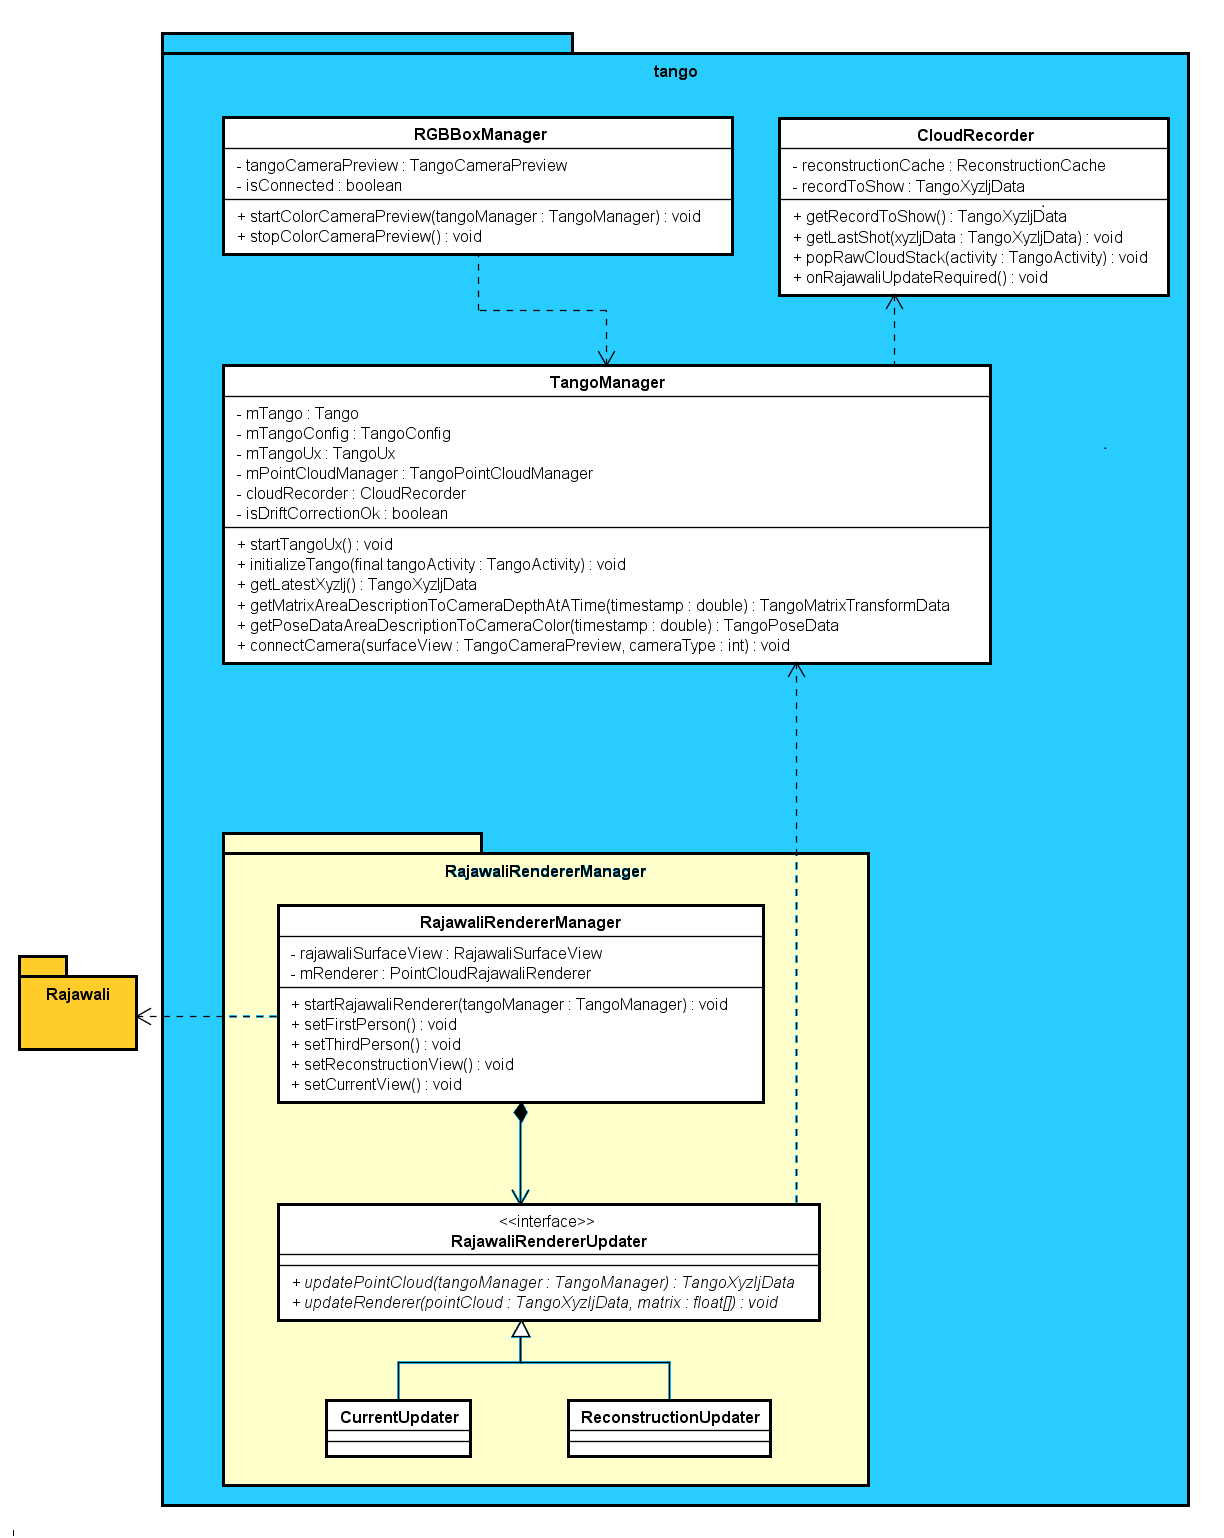
\includegraphics[width=1.0\columnwidth]{st/Samba_tango.png} 
    \caption{Componente Samba.tango}
\end{figure}
\subsubsection{Descrizione}
Questo \emph{package} contiene un insieme di classi che possono essere usate per interagire con il ciclo di vita dei sensori \emph{Tango} e del \emph{renderer} dei punti. Questi \emph{manager} possono essere usati per gestire la \emph{business logic} di una applicazione \emph{Tango} separandola dalla sua rappresentazione grafica.
\subsubsection{Package figli}
\begin{itemize}
	\item Samba.tango.RajawaliRendererManager
\end{itemize}
\subsubsection{Classi}
\begin{itemize}
	\item Samba.tango.RGBBoxManager
	\item Samba.tango.CloudRecorder
	\item Samba.tango.TangoManager
\end{itemize}

\subsection{Samba.tango.RajawaliRendererManager}
\subsubsection{Descrizione}
\emph{Package} che contiene il \emph{manager} per gestire il \emph{rendering} dei punti tramite la libreria \emph{Rajawali}.
\subsubsection{Interfacce}
\begin{itemize}
	\item Samba.tango.RajawaliRendererManager.RajawaliRendererUpdater
\end{itemize}
\subsubsection{Classi}
\begin{itemize}
	\item Samba.tango.RajawaliRendererManager.RajawaliRendererManager
	\item Samba.tango.RajawaliRendererManager.CurrentUpdater
	\item Samba.tango.RajawaliRendererManager.ReconstructionUpdater
\end{itemize}


\subsection{Samba.tango.RajawaliRendererManager.RajawaliRendererManager}
\subsubsection{Descrizione}
Questa classe permette di integrare un servizio di \emph{rendering} di \emph{Point Cloud} all'interno del ciclo di vita di una applicazione \emph{Andorid}. Oltre alla visualizzazione espone metodi per cambiare la modalità del \emph{render}, e di effettuare qualche azione sullo stesso.
\subsubsection{Utilizzo}
È utilizzata per fornire un \emph{render} nell'attività principale dell'applicazione prodotta. (Come quello in figura \ref{fig:render-rajawali} in tutta la parte destra dello schermo)
\subsubsection{Relazioni con altre classi}
\begin{itemize}
	\item \texttt{Samba.activity.tangoActivity.PointCloudActivity}: relazione entrante, composizione.
	\item \texttt{Samba.activity.tangoActivity.TangoActivity}: relazione uscente, dipendenza, utilizzo come parametro di uno o più metodi.
	\item \texttt{Samba.tango.RajawaliRendererManager.RajawaliRendererUpdater}: relazione uscente, composizione.
\end{itemize}

\subsection{Samba.tango.RajawaliRendererManager.RajawaliRendererUpdater}
\subsubsection{Descrizione}
Interfaccia che rappresenta il componente \emph{Strategy} del \emph{Desing Pattern} \emph{Strategy}.
\subsubsection{Utilizzo}
È usata per alternare la modalità del \emph{render} tra la rappresentazione in tempo reale dei dati del sensore e quella della ricostruzione corrente.
\subsubsection{Relazioni con altre classi}
\begin{itemize}
	\item \texttt{Samba.tango.RajawaliRendererManager.RajawaliRendererManager}: relazione entrante, composizione.
	\item \texttt{Samba.tango.TangoManager}: relazione uscente, dipendenza.
\end{itemize}
\subsubsection{Implementata da}
\begin{itemize}
	\item Samba.tango.RajawaliRendererManager.CurrentUpdater
	\item Samba.tango.RajawaliRendererManager.ReconstructionUpdater
\end{itemize}


\subsection{Samba.tango.RajawaliRendererManager.CurrentUpdater}
\subsubsection{Descrizione}
Implementazione di \emph{RajawaliRendererUpdater} che rappresenta la visione in tempo reale dei dati del sensore.
\subsubsection{Utilizzo}
È usata per impostare il \emph{render} alla modalità in tempo reale.
\subsubsection{Interfacce implementate}
\begin{itemize}
	\item Samba.tango.RajawaliRendererManager.RajawaliRendererUpdater
\end{itemize}

\subsection{Samba.tango.RajawaliRendererManager.ReconstructionUpdater}
\subsubsection{Descrizione}
Implementazione di \emph{RajawaliRendererUpdater} che rappresenta la visione del \emph{Point Cloud} correntemente ricostruito.
\subsubsection{Utilizzo}
È usata per impostare il \emph{render} alla modalità ricostruzione.
\subsubsection{Interfacce implementate}
\begin{itemize}
	\item Samba.tango.RajawaliRendererManager.RajawaliRendererUpdater
\end{itemize}

\subsection{Samba.tango.RGBBoxManager}
\subsubsection{Descrizione}
Questa classe permette di integrare un servizio di \emph{preview} della fotocamera all'interno del ciclo di vita di una applicazione \emph{Andorid}.
\subsubsection{Utilizzo}
È utilizzata per fornire una \emph{preview} della fotocamera nell'attività principale dell'applicazione prodotta. (Come quella in figura \ref{fig:render-rajawali} in basso a sinistra)
\subsubsection{Relazioni con altre classi}
\begin{itemize}
	\item \texttt{Samba.activity.tangoActivity.PointCloudActivity}: relazione entrante, composizione.
	\item \texttt{Samba.activity.tangoActivity.TangoActivity}: relazione uscente, dipendenza, utilizzo come parametro di uno o più metodi.
	\item \texttt{Samba.tango.TangoManager}: relazione uscente, dipendenza.
\end{itemize}

\subsection{Samba.tango.TangoManager}
\subsubsection{Descrizione}
Questa classe permette di integrare i servizi \emph{Tango} all'interno del ciclo di vita di una applicazione \emph{Andorid}. Inoltre imposta correttamente il \emph{framework} \emph{TangoUx} e fornisce metodi per ricavare statistiche e dati algebrici.
\subsubsection{Utilizzo}
È utilizzata per fornire all'attività principale dell'applicazione prodotta la possibilità di sfruttare i servizi \emph{Tango}.
\subsubsection{Relazioni con altre classi}
\begin{itemize}
	\item \texttt{Samba.activity.tangoActivity.PointCloudActivity}: relazione entrante, composizione.
	\item \texttt{Samba.activity.tangoActivity.TangoActivity}: relazione uscente, dipendenza, utilizzo come parametro di uno o più metodi.
	\item \texttt{Samba.tango.RGBBoxManager}: relazione entrante, dipendenza.
	\item \texttt{Samba.tango.RajawaliRendererManager.RajawaliRendererUpdater}: relazione entrante, dipendenza.
	\item \texttt{Samba.tango.CloudRecorder}: relazione uscente, dipendenza.
	\item \texttt{Samba.clouds.utils.poseSanity.PoseSanityChecker}: relazione uscente, composizione.
	\item \texttt{Samba.clouds.utils.poseSanity.PoseDriftCorrectionStatus}: relazione uscente, dipendenza.
\end{itemize}

\subsection{Samba.tango.CloudRecorder}
\subsubsection{Descrizione}
Mantiene la ricostruzione corrente in un formato comprensibile dal \emph{renderer}.
\subsubsection{Utilizzo}
Viene usata per effettuare il \emph{rendering} del \emph{Point Cloud} della ricostruzione corrente.
\subsubsection{Relazioni con altre classi}
\begin{itemize}
	\item \texttt{Samba.activity.tangoActivity.PointCloudActivity}: relazione entrante, composizione.
	\item \texttt{Samba.activity.tangoActivity.TangoActivity}: relazione uscente, dipendenza, utilizzo come parametro di uno o più metodi.
	\item \texttt{Samba.tango.TangoManager}: relazione entrante, dipendenza.
	\item \textbf{Samba.sharedState.ReconstructionCache}: relazione uscente, composizione.
	\item \texttt{Samba.clouds.utils.SambaRawData}: relazione uscente, dipendenza.
	\item \texttt{Samba.utils.encoding.EcnodeStrategy}: relazione uscente, composizione.
\end{itemize}


\subsection{Samba.sharedState}
\begin{figure}[!h] 
    \centering 
    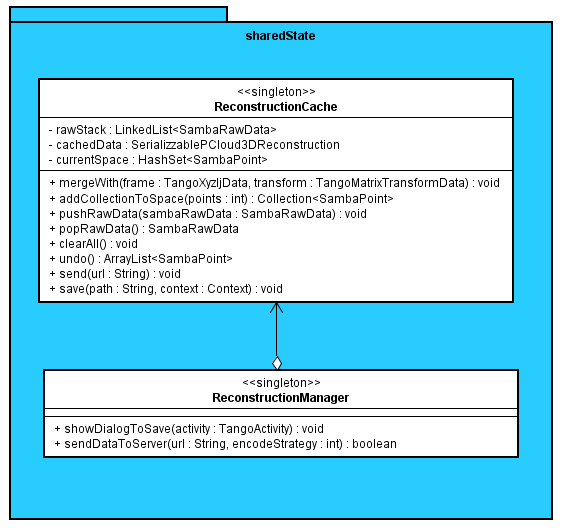
\includegraphics[width=0.9\columnwidth]{st/Samba_sharedState.png} 
    \caption{Componente Samba.sharedState}
\end{figure}
\subsubsection{Descrizione}
Questo \emph{package} contiene un \emph{singleton} che mantiene tutti gli stati condivisi tra i vari servizi e una classe di utilità.
\subsubsection{Classi}
\begin{itemize}
	\item Samba.sharedState.ReconstructionCache
	\item Samba.sharedState.ReconstructionManager
\end{itemize}

\subsection{Samba.sharedState.ReconstructionCache}
\subsubsection{Descrizione}
Questo \emph{singleton} mantiene tutte le informazioni condivise tra i vari servizi asincroni presenti nell'applicazione. Fornisce tutti i metodi necessari per accedervi controllatamente, e si occupa anche di sincronizzare gli accessi stessi dove necessario.
\subsubsection{Utilizzo}
È usata dai servizi presenti nell'applicazione per salvare e modificare i loro stati condivisi.
\subsubsection{Relazioni con altre classi}
\begin{itemize}
	\item \texttt{Samba.sharedState.ReconstructionManager}: relazione entrante, aggregazione.
	\item \texttt{Samba.activity.ObjectChooseActivity}: relazione entrante, composizione.
	\item \texttt{Samba.activity.tangoActivity.PointCloudActivity}: relazione entrante, composizione.
	\item \texttt{Samba.tango.CloudRecorder}: relazione entrante, composizione.
	\item \texttt{Samba.utils.services.MergingService}: relazione entrante, composizione.
	\item \texttt{Samba.utils.services.VoxelService}: relazione entrante, composizione.	
	\item \texttt{Samba.clouds.reconstruction.UndoableReconstruction}: relazione uscente, dipendenza, controllo di tipo.
	\item \texttt{Samba.clouds.utils.SambaPoint}: relazione uscente, dipendenza.
	\item \texttt{Samba.clouds.utils.SambaRawData}: relazione uscente, composizione.
	\item \texttt{Samba.utils.sending.ReconstructionSender}: relazione uscente, composizione.
	\item \texttt{Samba.utils.sending.ArrListSender}: relazione uscente, composizione.	
\end{itemize}

\subsection{Samba.sharedState.ReconstructionManager}
\subsubsection{Descrizione}
\emph{Singleton} di utilità che fornisce delle \emph{macro} per sequenze di operazioni effettuate ricorrentemente su \emph{ReconstructionCache}.
\subsubsection{Utilizzo}
Viene usato da alcuni componenti per effettuare complesse operazioni sullo stato condiviso.
\subsubsection{Relazioni con altre classi}
\begin{itemize}
	\item \texttt{Samba.sharedState.ReconstructionCache}: relazione uscente, aggregazione.
	\item \texttt{Samba.activity.tangoActivity.PointCloudActivity}: relazione entrante, composizione.	
\end{itemize}


\subsection{Samba.clouds}
\begin{figure}[!h] 
    \centering 
    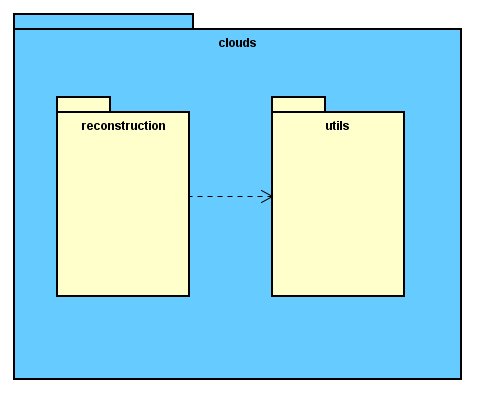
\includegraphics[width=0.8\columnwidth]{st/Samba_clouds.png} 
    \caption{Componente Samba.clouds}
\end{figure}
\subsubsection{Descrizione}
Questo \emph{package} contiene tutte le strutture dati usate per rappresentare internamente i \emph{Point Cloud}.
\subsubsection{Package figli}
\begin{itemize}
	\item Samba.clouds.reconstruction
	\item Samba.clouds.utils
\end{itemize}


\subsection{Samba.clouds.reconstruction}
\begin{figure}[!h] 
    \centering 
    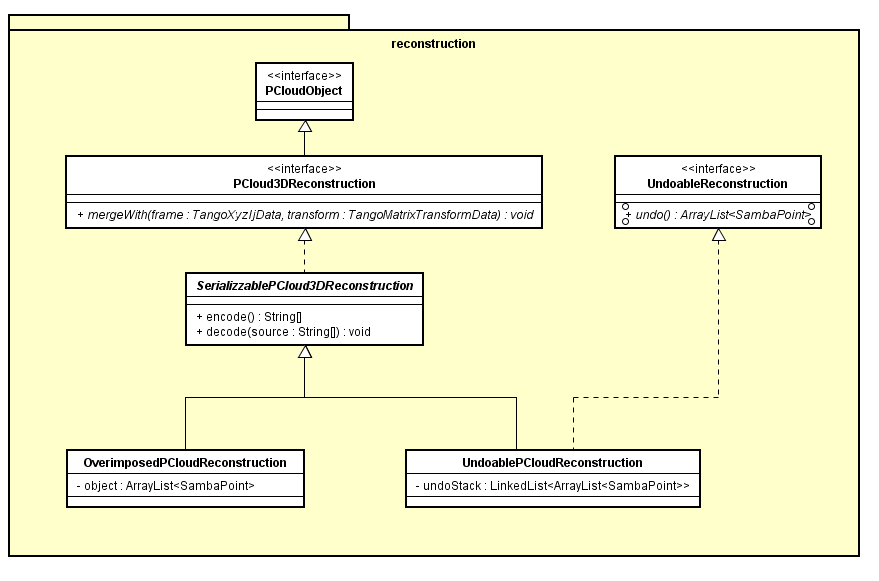
\includegraphics[width=1.0\columnwidth]{st/Samba_clouds_reconstruction.png} 
    \caption{Componente Samba.reconstruction}
\end{figure}
\subsubsection{Descrizione}
Per motivi di ottimizzazione si è cercato di lasciare il più possibile aperte le possibilità di modifica della rappresentazione interna dei \emph{Point Cloud} ricostruiti. Questo \emph{package} contiene tutte le classi che rappresenta un \emph{Point Cloud} ricostruito.
\subsubsection{Interfacce}
\begin{itemize}
	\item Samba.clouds.PCloudObject
	\item Samba.clouds.PCloud3DReconstruction
	\item Samba.clouds.UndoableReconstruction
\end{itemize}
\subsubsection{Classi}
\begin{itemize}
	\item Samba.clouds.OverimposedPCloudReconstruction
	\item Samba.clouds.UndoablePCloudReconstruction
\end{itemize}

\subsection{Samba.clouds.reconstruction.PCloudObject}
\subsubsection{Descrizione}
Rappresenta un generico oggetto 3D rappresentato tramite \emph{Point Cloud}.
\subsubsection{Utilizzo}
È utilizzato come interfaccia alla base della gerarchia dei possibili \emph{Point Cloud}.
\subsubsection{Estesa da}
\begin{itemize}
	\item Samba.clouds.reconstruction.PCloud3DReconstruction
\end{itemize}

\subsection{Samba.clouds.reconstruction.PCloud3DReconstruction}
\subsubsection{Descrizione}
Interfaccia che rappresenta un generico \emph{Point Cloud} in grado di essere sovrapposto ad altre nuvole di punti per creare un oggetto tridimensionale completo.
\subsubsection{Utilizzo}
È usata come interfaccia alla base della gerarchia delle possibili ricostruzioni 3D.
\subsubsection{Interfacce estese}
\begin{itemize}
	\item Samba.clouds.reconstruction.PCloudObject
\end{itemize}
\subsubsection{Implementata da}
\begin{itemize}
	\item Samba.clouds.reconstruction.SerializzablePCloud3DReconstruction
\end{itemize}

\subsection{Samba.clouds.reconstruction.UndoableReconstruction}
\subsubsection{Descrizione}
Interfaccia che espone i metodi necessari per permettere ad una ricostruzione di effettuare operazioni di \emph{undo}. Una \emph{UndoableReconstruction} \textbf{non} è una \emph{PCloud3DReconstrucion}. 
\subsubsection{Utilizzo}
È implementata dalle classi che rappresentano una ricostruzione 3D e che necessitano operazioni di \emph{undo}.
\subsubsection{Relazioni con altre classi}
\begin{itemize}
	\item \texttt{Samba.sharedState.ReconstructionCache}: relazione entrante, dipendenza, controllo di tipo.
	\item \texttt{Samba.clouds.utils.SambaPoint}: relazione uscente, dipendenza.
\end{itemize}
\subsubsection{Implementata da}
\begin{itemize}
	\item Samba.clouds.reconstruction.UndoablePCloudReconstruction
\end{itemize}


\subsection{Samba.clouds.reconstruction.SerializzablePCloud3DReconstruction}
\subsubsection{Descrizione}
Classe astratta che rappresenta un generico \emph{Point Cloud} in grado di essere sovrapposto ad altre nuvole di punti per creare un oggetto tridimensionale completo ed che può essere inoltre serializzato per salvarlo su disco o inviarlo ad un \emph{Server}.
\subsubsection{Utilizzo}
È usata come classe astratta base della gerarchia delle possibili ricostruzioni 3D.
\subsubsection{Relazioni con altre classi}
\begin{itemize}
	\item \texttt{Samba.utils.encoding.EncodeStrategy}: relazione uscente, composizione.
	\item \texttt{Samba.sharedState.ReconstructionCache}: relazione entrante, composizione.
	\item \texttt{Samba.utils.sending.ReconstructionSender}: relazione entrante, composizione.
	\item \texttt{Samba.clouds.utils.SambaPoint}: relazione uscente, dipendenza.
	\item \texttt{Samba.utils.encoding.EcnodeStrategy}: relazione uscente, composizione.
\end{itemize}
\subsubsection{Interfacce implementate}
\begin{itemize}
	\item Samba.clouds.reconstruction.PCloud3DReconstruction
\end{itemize}
\subsubsection{Estesa da}
\begin{itemize}
	\item Samba.clouds.reconstruction.OverimposedPCloudReconstruction
	\item Samba.clouds.reconstruction.UndoablePCloudReconstruction
\end{itemize}

\subsection{Samba.clouds.reconstruction.OverimposedPCloudReconstruction}
\subsubsection{Descrizione}
Rappresenta una ricostruzione 3D in cui i \emph{Point Cloud} sono semplicemente sovrapposti senza alcuna ulteriore ottimizzazione.
\subsubsection{Utilizzo}
Attualmente non è usata in favore di \emph{UndoablePCloudReconstruction} (vedi \ref{class:UndoablePCloudReconstruction}).
\subsubsection{Relazioni con altre classi}
\begin{itemize}
	\item \texttt{Samba.clouds.utils.Vector4}: relazione uscente, dipendenza.
	\item \texttt{Samba.clouds.utils.SambaPoint}: relazione uscente, dipendenza.
\end{itemize}
\subsubsection{Classi estese}
\begin{itemize}
	\item Samba.clouds.reconstruction.SerializzablePCloud3DReconstruction
\end{itemize}

\subsection{Samba.clouds.reconstruction.UndoablePCloudReconstruction}
\label{class:UndoablePCloudReconstruction}
\subsubsection{Descrizione}
Rappresenta una ricostruzione 3D in cui i \emph{Point Cloud} sono semplicemente sovrapposti ma con la possibilità di annullare un certo numero di operazioni.
\subsubsection{Utilizzo}
È usata come tipo preferito per contenere i dati dell'oggetto ricostruito, una volta elaborati, ma non ancora \emph{voxellati}.
\subsubsection{Relazioni con altre classi}
\begin{itemize}
	\item \texttt{Samba.clouds.utils.Vector4}: relazione uscente, dipendenza.
	\item \texttt{Samba.clouds.utils.SambaPoint}: relazione uscente, dipendenza.
\end{itemize}
\subsubsection{Interfacce implementate}
\begin{itemize}
	\item Samba.clouds.reconstruction.UndoableReconstruction
\end{itemize}
\subsubsection{Classi estese}
\begin{itemize}
	\item Samba.clouds.reconstruction.SerializzablePCloud3DReconstruction
\end{itemize}


\subsection{Samba.clouds.utils}
\begin{figure}[!h] 
    \centering 
    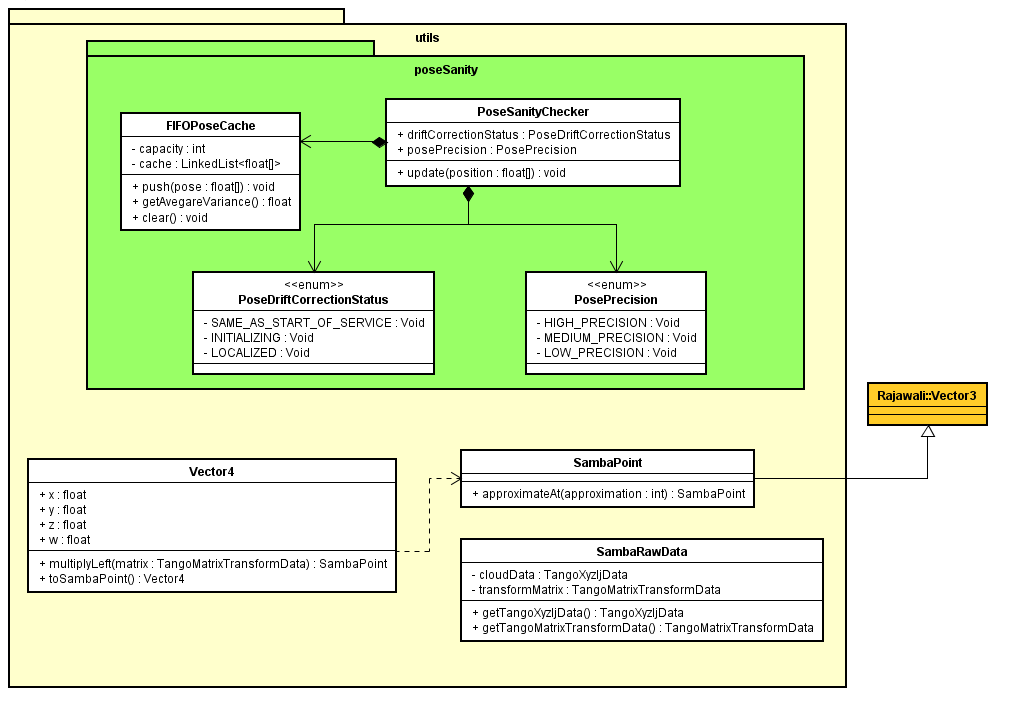
\includegraphics[width=1.0\columnwidth]{st/Samba_clouds_utils.png} 
    \caption{Componente Samba.clouds.utils}
\end{figure}
\subsubsection{Descrizione}
Contiene tutte le strutture dati di utilità usate per rappresentazione interna, come punti, \emph{Point Cloud} uniti alla propria matrice associata etc.
\subsubsection{Package figli}
\begin{itemize}
	\item Samba.clouds.utils.poseSanity
\end{itemize}
\subsubsection{Classi}
\begin{itemize}
	\item Samba.clouds.utils.Vector4
	\item Samba.clouds.utils.SambaPoint
	\item Samba.clouds.utils.SambaRawData
\end{itemize}

\subsection{Samba.clouds.utils.poseSanity}
\subsubsection{Descrizione}
Questo \emph{package} contiene le classi necessarie per effettuare il \emph{sanity check} della fase di localizzazione.
\subsubsection{Classi}
\begin{itemize}
	\item Samba.clouds.utils.poseSanity.PoseSanityChecker
	\item Samba.clouds.utils.poseSanity.FIFOPoseCache
\end{itemize}
\subsubsection{Enumerazioni}
\begin{itemize}
	\item Samba.clouds.utils.poseSanity.PoseDriftCorrectionStatus
	\item Samba.clouds.utils.poseSanity.PosePrecision
\end{itemize}

\subsection{Samba.clouds.utils.poseSanity.PoseSanityChecker}
\label{class:PoseSanityChecker}
\subsubsection{Descrizione}
Questa classe fornisce un \emph{sanity check} della fase di localizzazione.
\subsubsection{Utilizzo}
È utilizzata durante la fase di localizzazione per tenere traccia dello stato della stessa. Inoltre è usata per fornire una stima di quanto la localizzazione stessa sia avvenuta in maniera precisa.
\subsubsection{Relazioni con altre classi}
\begin{itemize}
	\item \texttt{Samba.clouds.utils.poseSanity.FIFOPoseCache}: relazione uscente, composizione.
	\item \texttt{Samba.clouds.utils.poseSanity.PoseDriftCorrectionStatus}: relazione uscente, composizione.
	\item \texttt{Samba.clouds.utils.poseSanity.PosePrecision}: relazione uscente, composizione.
	\item \texttt{Samba.tango.TangoManager}: relazione entrante, composizione.
\end{itemize}

\subsection{Samba.clouds.utils.poseSanity.FIFOPoseCache}
\subsubsection{Descrizione}
Fornisce una cosa \emph{FIFO} in grado di tenere in memoria le ultime $n$ posizioni rilevate e usarle per dei calcoli statistici in maniera efficiente.
\subsubsection{Utilizzo}
È usata come classe di utilità per \texttt{PoseSanityChecker} (\ref{class:PoseSanityChecker}).
\subsubsection{Relazioni con altre classi}
\begin{itemize}
	\item \texttt{Samba.clouds.utils.poseSanity.PoseSanityChecker}: relazione entrante, composizione.
\end{itemize}

\subsection{Samba.clouds.utils.poseSanity.PoseDriftCorrectionStatus}
\subsubsection{Descrizione}
Enumerazione che rappresenta i possibili stati della \emph{Drift Correction}, quelli discussi in \ref{cap:istruzioni-per-utente} alla voce "Istruzioni per l'utente".
\subsubsection{Valori}
\begin{itemize}
	\item \texttt{SAME\_AS\_START\_OF\_SERVICE}
	\item \texttt{INITIALIZING}
	\item \texttt{LOCALIZED}		
\end{itemize}
\subsubsection{Relazioni con altre classi}
\begin{itemize}
	\item \texttt{Samba.clouds.utils.poseSanity.poseSanityChecker}: relazione entrante, composizione.
	\item \texttt{Samba.tango.TangoManager}: relazione entrante, dipendenza.
\end{itemize}


\subsection{Samba.clouds.utils.poseSanity.PosePrecision}
\subsubsection{Descrizione}
Enumerazione che rappresenta i possibili livelli di precisione a cui è avvenuta la localizzazione.
\subsubsection{Valori}
\begin{itemize}
	\item \texttt{HIGH\_PRECISION}
	\item \texttt{MEDIUM\_PRECISION}
	\item \texttt{LOW\_PRECISION}		
\end{itemize}
\subsubsection{Relazioni con altre classi}
\begin{itemize}
	\item \texttt{Samba.clouds.utils.poseSanity.poseSanityChecker}: relazione entrante, composizione.
	\item \texttt{Samba.activity.tangoActivity.OnTangoUiUpdateListener}: relazione entrante, dipendenza, utilizzo come parametro di uno o più metodi.
\end{itemize}

\subsection{Samba.clouds.utils.Vector4}
\subsubsection{Descrizione}
Classe che rappresenta un vettore di quattro dimensioni. Offre i metodi necessari per i calcoli del sistema.
\subsubsection{Utilizzo}
È usato per adattare l'interfaccia di un vettore a tre dimensioni quando è necessario moltiplicarlo per una matrice di trasformazione di un \emph{Point Cloud} (che ha quattro dimensioni).
\subsubsection{Relazioni con altre classi}
\begin{itemize}
	\item \texttt{Samba.clouds.utils.SambaPoint}: relazione uscente, dipendenza, utilizzo come parametro di uno o più metodi.
	\item \texttt{Samba.cloud.reconstruction.OverimposedPCloudReconstruction}: relazione entrante, dipendenza.
	\item \texttt{Samba.cloud.reconstruction.UndoablePCloudReconstruction}: relazione entrante, dipendenza.	
\end{itemize}

\subsection{Samba.clouds.utils.SambaPoint}
\subsubsection{Descrizione}
Questa classe rappresenta un punto all'interno di un \emph{PointCloud}. È un \emph{wrapper} di \texttt{Vector3} della libreria \emph{Rajawali}. Espone quindi le stesse funzionalità ma ne aggiunge altre di indispensabili, come essere confrontabile ed essere \emph{parcellabile}. È stato scelto di creare questo \emph{wrapper} proprio perché \texttt{Vector3} non forniva queste caratteristiche.
\subsubsection{Utilizzo}
È utilizzata ovunque sia richiesto il concetto di \emph{punto} all'interno del sistema.
\subsubsection{Relazioni con altre classi}
\begin{itemize}
	\item \texttt{Samba.clouds.utils.Vector4}: relazione entrante, dipendenza.
	\item \texttt{Samba.activity.ObjectChooseActivity}: relazione entrante, dipendenza.
	\item \texttt{Samba.activity.tangoActivity.PointCloudActivity}:	relazione entrante, dipendenza.
	\item \texttt{Samba.clouds.reconstruction.UndoableReconstruction}: relazione entrante, dipendenza.
	\item \texttt{Samba.clouds.reconstruction.SerializzablePCloud3DReconstruction}: relazione entrante, dipendenza.
	\item \texttt{Samba.clouds.reconstruction.OverimposedPCloudReconstruction}: relazione entrante, dipendenza.
	\item \texttt{Samba.clouds.reconstruction.UndoablePCloudReconstruction}: relazione entrante, dipendenza.
	\item \texttt{Samba.sharedState.ReconstructionCache}: relazione entrante, dipendenza.
	\item \texttt{Samba.utils.encoding.EncodeStrategy}: relazione entrante, dipendenza.
	\item \texttt{Samba.utils.encoding.XyzEncoder}: relazione entrante, dipendenza.
	\item \texttt{Samba.utils.encoding.PcdEncoder}: relazione entrante, dipendenza.
	\item \texttt{Samba.utils.sending.ArrListSender}: relazione entrante, dipendenza.
	\item \texttt{Samba.utils.sending.InternalStorageSender}: relazione entrante, dipendenza.
	\item \texttt{Samba.utils.services.VoxelService}: relazione entrante, dipendenza.
\end{itemize}
\subsubsection{Classi estese}
\begin{itemize}
	\item org.rajawali3d.math.vector.Vector3
\end{itemize}

\subsection{Samba.clouds.utils.SambaRawData}
\subsubsection{Descrizione}
Classe che permette di impacchettare assieme un \texttt{TangoXyzIjData} (dati del sensore di profondità \emph{Tango}) e la sua matrice di rotazione.
\subsubsection{Utilizzo}
È usata ovunque ci sia bisogno di mantenere dei dati "grezzi" prima di effettuare rotazione e traslazione.
\subsubsection{Relazioni con altre classi}
\begin{itemize}
	\item \texttt{Samba.sharedState.ReconstructionCache}: relazione entrante, composizione.
	\item \texttt{Samba.tango.CloudRecorder}: relazione entrante, dipendenza, utilizzo come parametro di uno o più metodi.
	\item \texttt{Samba.utils.services.MergingService}: relazione entrante, dipendenza, utilizzo interno ad un metodo.	
\end{itemize}


\subsection{Samba.utils}
\begin{figure}[!h] 
    \centering 
    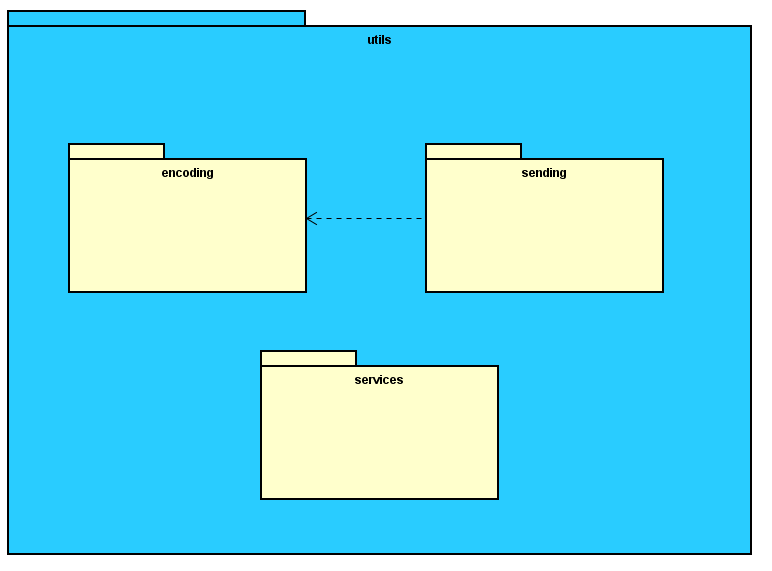
\includegraphics[width=0.9\columnwidth]{st/Samba_utils.png} 
    \caption{Componente Samba.utils}
\end{figure}
\subsubsection{Descrizione}
Questo \emph{package} contiene classi di utilità generale.
\subsubsection{Package figli}
\begin{itemize}
	\item Samba.utils.encoding
	\item Samba.utils.sending
	\item Samba.utils.services
\end{itemize}


\subsection{Samba.utils.encoding}
\begin{figure}[!h] 
    \centering 
    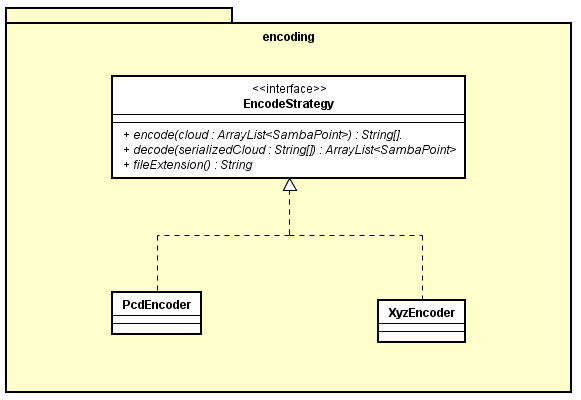
\includegraphics[width=1.0\columnwidth]{st/Samba_utils_encoding.png} 
    \caption{Componente Samba.utils.encoding}
\end{figure}
\subsubsection{Descrizione}
Questo \emph{package} contiene le classi necessarie serializzare e deserializzare i \emph{Point Cloud}.
\subsubsection{Interfacce}
\begin{itemize}
	\item Samba.utils.encoding.EncodeStrategy
\end{itemize}
\subsubsection{Classi}
\begin{itemize}
	\item Samba.utils.encoding.PcdEncoder
	\item Samba.utils.encoding.XyzEncoder
\end{itemize}

\subsection{Samba.utils.encoding.EcnodeStrategy}
\subsubsection{Descrizione}
Interfaccia che rappresenta la strategia con cui effettuare l'\emph{encoding} di un \emph{Point Cloud}.
\subsubsection{Utilizzo}
È usata come componente \emph{Strategy} di uno \emph{Strategy Pattern}.
\subsubsection{Relazioni con altre classi}
\begin{itemize}
	\item \texttt{Samba.activity.ObjectChooseActivity}: relazione entrante, composizione.
	\item \texttt{Samba.clouds.reconstruction.SerializzablePCloud3DReconstruction}: relazione entrante, composizione.
	\item \texttt{Samba.utils.sending.ArrListSender}: relazione entrante, composizione.
	\item \texttt{Samba.utils.sending.ReconstructionSender}: relazione entrante, composizione.	
\end{itemize}
\subsubsection{Implementata da}
\begin{itemize}
	\item Samba.utils.encoding.PcdEncoder
	\item Samba.utils.encoding.XyzEncoder
\end{itemize}

\subsection{Samba.utils.encoding.PcdEncoder}
\subsubsection{Descrizione}
Implementazione della strategia di \emph{encoding} che serializza i \emph{Point Cloud} in formato \emph{pcd}.
\subsubsection{Utilizzo}
È il formato preferito dal sistema per salvare e spedire i \emph{file}.
\subsubsection{Interfacce implementate}
\begin{itemize}
	\item Samba.clouds.reconstruction.EcnodeStrategy
\end{itemize}

\subsection{Samba.utils.encoding.PcdEncoder}
\subsubsection{Descrizione}
Implementazione della strategia di \emph{encoding} che serializza i \emph{Point Cloud} in formato \emph{xyz}.
\subsubsection{Utilizzo}
È un formato non utilizzato nel sistema.
\subsubsection{Interfacce implementate}
\begin{itemize}
	\item Samba.clouds.reconstruction.EcnodeStrategy
\end{itemize}


\subsection{Samba.utils.sending}
\begin{figure}[!h] 
    \centering 
    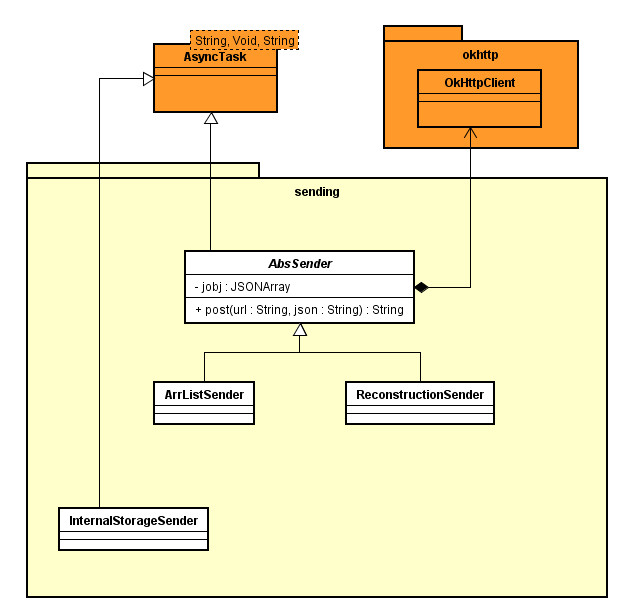
\includegraphics[width=1.0\columnwidth]{st/Samba_utils_sending.png} 
    \caption{Componente Samba.utils.sending}
\end{figure}
\subsubsection{Descrizione}
Questo \emph{package} contiene delle \emph{AsyncTask} che hanno il compito di spedire un \emph{Point Cloud} serializzato ad un \emph{Server} oppure di salvarlo su disco.
\subsubsection{Classi}
\begin{itemize}
	\item Samba.utils.sending.AbsSender
	\item Samba.utils.sending.ArrListSender
	\item Samba.utils.sending.ReconstructionSender
	\item Samba.utils.sending.InternalStorageSender
\end{itemize}

\subsection{Samba.utils.sending.AbsSender}
\subsubsection{Descrizione}
Classe astratta per inviare un \emph{Point Cloud} tramite \emph{http} in un \emph{thread} separato dal resto dell'applicazione.
\subsubsection{Classi estese}
\begin{itemize}
	\item android.os.AsyncTask
\end{itemize}
\subsubsection{Estesa da}
\begin{itemize}
	\item Samba.utils.sending.ArrListSender
	\item Samba.utils.sending.ReconstructionSender
\end{itemize}

\subsection{Samba.utils.sending.ArrListSender}
\subsubsection{Descrizione}
Classe in grado di inviare liste di \texttt{SambaPoint}.
\subsubsection{Utilizzo}
È usata per inviare liste di \texttt{SambaPoint}.
\subsubsection{Relazioni con altre classi}
\begin{itemize}
	\item \texttt{Samba.clouds.utils.SambaPoint}: relazione uscente, dipendenza.
	\item \texttt{Samba.utils.encoding.EncodeStrategy}: relazione uscente, composizione.
	\item \texttt{Samba.sharedState.ReconstructionCache}: relazione entrante, composizione.
\end{itemize}
\subsubsection{Classi estese}
\begin{itemize}
	\item Samba.utils.sending.AbsSender
\end{itemize}

\subsection{Samba.utils.sending.ReconstructionSender}
\subsubsection{Descrizione}
Classe in grado di inviare ricostruzioni 3D.
\subsubsection{Utilizzo}
È usata per inviare ricostruzioni 3D.
\subsubsection{Relazioni con altre classi}
\begin{itemize}
	\item \texttt{Samba.clouds.utils.SambaPoint}: relazione uscente, dipendenza.
	\item \texttt{Samba.utils.encoding.EncodeStrategy}: relazione uscente, composizione.
	\item \texttt{Samba.sharedState.ReconstructionCache}: relazione entrante, composizione.
\end{itemize}
\subsubsection{Classi estese}
\begin{itemize}
	\item Samba.utils.sending.AbsSender
\end{itemize}

\subsection{Samba.utils.sending.InternalStorageSender}
\subsubsection{Descrizione}
Classe in grado di salvare su disco \emph{Point Cloud} serializzati.
\subsubsection{Utilizzo}
È usata per salvare su disco \emph{Point Cloud} serializzati.
\subsubsection{Relazioni con altre classi}
\begin{itemize}
	\item \texttt{Samba.clouds.utils.SambaPoint}: relazione uscente, dipendenza.
	\item \texttt{Samba.utils.encoding.EncodeStrategy}: relazione uscente, composizione.
	\item \texttt{Samba.sharedState.ReconstructionCache}: relazione entrante, composizione.
\end{itemize}

\subsection{Samba.utils.services}
\begin{figure}[!h] 
    \centering 
    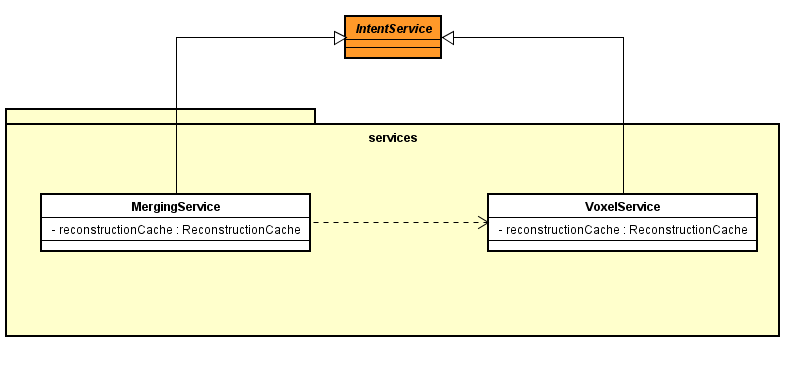
\includegraphics[width=1.0\columnwidth]{st/Samba_utils_services.png} 
    \caption{Componente Samba.utils.services}
\end{figure}
\subsubsection{Descrizione}
Questo \emph{package} contiene i servizi asincroni che servono ad effettuare operazioni sui dati raccolti dai sensori \emph{Tango}.
\subsubsection{Classi}
\begin{itemize}
	\item Samba.utils.services.MergingService
	\item Samba.utils.services.VoxelService
\end{itemize}

\subsection{Samba.utils.services.MergingService}
\subsubsection{Descrizione}
Servizio in grado di sovrapporre ad una ricostruzione data un \emph{Point Cloud} a patto che assieme a quest'ultimo venga fornita anche la sua matrice di trasformazione.
\subsubsection{Utilizzo}
È usato per ricostruire in \emph{backgroud} l'oggetto inquadrato dall'utente.
\subsubsection{Relazioni con altre classi}
\begin{itemize}
	\item \texttt{Samba.clouds.utils.SambaRawData}: relazione uscente, dipendenza, utilizzo interno ad un metodo.
	\item \texttt{Samba.utils.services.VoxelService}: relazione uscente, dipendenza.
\end{itemize}
\subsubsection{Classi estese}
\begin{itemize}
	\item android.app.IntentService
\end{itemize}

\subsection{Samba.utils.services.VoxelService}
\subsubsection{Descrizione}
Servizio in grado di ottimizzare una ricostruzione 3D eliminando i punti ridondanti.
\subsubsection{Utilizzo}
È usato in \emph{backgroud} ottimizzare ed eliminare i punti ridondanti da una ricostruzione 3D.
\subsubsection{Relazioni con altre classi}
\begin{itemize}
	\item \texttt{Samba.clouds.utils.SambaPoint}: relazione uscente, dipendenza, utilizzo interno ad un metodo.
	\item \texttt{Samba.utils.services.MergingService}: relazione entrante, dipendenza.
\end{itemize}
\subsubsection{Classi estese}
\begin{itemize}
	\item android.app.IntentService
\end{itemize}


%**************************************************************
\section{Design Pattern utilizzati}

%**************************************************************
\section{Codifica}
             % Product Prototype
% !TEX encoding = UTF-8
% !TEX TS-program = pdflatex
% !TEX root = ../tesi.tex
% !TEX spellcheck = it-IT

%**************************************************************
\chapter{Verifica e validazione}
\label{cap:verifica-validazione}
%**************************************************************

\section{Test di Unità}
xxxx
\section{Test di Integrazione}
xxxx
\section{Test di Sistema}
Data la natura prototipale del progetto ai test di Sistema è stata riservata una grande attenzione. Durante lo sviluppo dei prototipi giocattolo e comunque durante tutta la fase di progettazione e ed ideazione è stata continuamente incrementato un documento nella \emph{wiki} interna all'azienda al fine di immagazzinare li tutti i test di sistema che devono essere soddisfatti prima di ritenere "buono" un prototipo.
Segue la lista di tutti i Test di Sistema con relativo stato di soddisfacimento o meno.
\LTXtable{\textwidth}{tabelle/test/sistema.tex}              % Product Design Freeze e SOP
% !TEX encoding = UTF-8
% !TEX TS-program = pdflatex
% !TEX root = ../tesi.tex
% !TEX spellcheck = it-IT

%**************************************************************
\chapter{Conclusioni}
\label{cap:conclusioni}
%**************************************************************
Al di là del formalismo informatico, lo scopo principale di questo progetto era indagare sul possibile uso della tecnologia \emph{Tango} nel campo ispettivo come effettivo supporto allo studio di beni materiali. Il prototipo realizzato sembra confermare che cioè è possibile.\\
I risultati ottenuti sono stati piuttosto soddisfacenti e con qualche raffinamento appare possibile inserire l'applicazione in un contesto produttivo.

\section{Prove pratiche}
Il prototipo prodotto è stato testato in numerosi ambienti e su diversi oggetti. Nella quasi totalità dei casi i risultati sono stati più che sufficienti per quanto riguarda la qualità del \emph{Point Cloud} ricostruito.\\
Per quanto riguarda invece il calcolo del volume i risultati non sono ancora totalmente sufficienti: il volume ottenuto è sempre dello stesso ordine di grandezza del volume reale, ma spesso è affetto da un errore relativo tra il 30 ed il 50\% ed un errore del genere non è affatto tollerabile. Tale divario però è facilmente appianabile migliorando la qualità delle elaborazioni dei \emph{Point Cloud} e delle \emph{mesh} lato \emph{Server}.

\section{Sviluppi futuri}
Il progetto è nato molto recentemente, dopo circa due mesi di sviluppo è stato prodotto un prototipo soddisfacente. Molti dei problemi riscontrati durante il percorso di \emph{stage} sono stati risolti, grazie ai prototipi e alle prove pratiche sono state molteplici anche le idee per rendere l'applicazione ancora più completa. Riporto qui solo alcune di queste.

\subsection{ICP su tablet}\label{subs:ICP}
Uno più gravi problemi delle ricostruzioni 3D effettuate tramite sovrapposizione di \emph{Point Cloud} è il \emph{ghosting}. Si tratta dello sdoppiamento di alcune "facce" dell'oggetto ricostruito.\\
\begin{figure}[!h] 
    \centering 
    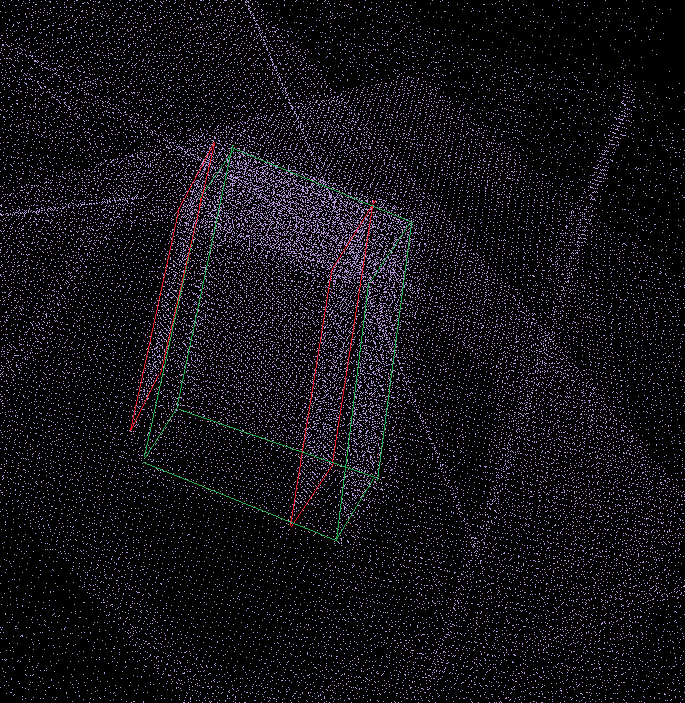
\includegraphics[width=0.9\columnwidth]{pointClouds/ghosting.png} 
    \caption{Point Cloud che presenta problemi di \emph{ghosting} di una scatola rettangolare}
    \label{figure:pcloud_ghosting}
\end{figure}
Nell'esempio in figura \ref{figure:pcloud_ghosting} sono stati evidenziati in verde gli spigoli corretti di una scatola rettangolare, mentre con colore rosso quelli dovuti al \emph{ghosting}; si può chiaramente notare che le facce laterali appaiono sdoppiate e ciò può portare a significativi errori nella ricostruzione dell'oggetto e soprattutto nel calcolo del volume.\\
Questo fenomeno è dovuto ad errori di stima nella posizione del dispositivo, e per quanto si cerchi di ridurli essi rimarranno sempre. Si tratta di un altro limite fisico dei dispositivi \emph{Tango}, che in questo caso è aggirabile.\\
\emph{ICP} o \emph{Iterative Closest Point} è un algoritmo che cerca di minimizzare le differenze tra due nuvole di punti. Applicando \emph{ICP} su due \emph{Point Cloud} che non si sovrappongono perfettamente permetterebbe di ottenere una matrice di trasformazione da applicare ad uno dei due per farlo combaciare all'altro. L'algoritmo in questione ha molte implementazioni in \emph{C++}, tra cui una presente proprio all'interno della libreria \emph{PCD} utilizzata lato \emph{Server}. Questo fatto ha dato modo di testare la sua effettiva efficacia.\\
Il problema è che spedire ogni singola ripresa al \emph{Server} ed aspettare una risposta sembra una strada non percorribile: per una rilevazione intera servono più di 20 riprese, senza connessione internet il servizio non sarebbe disponibile etc.\\
Per questo un possibile sviluppo futuro potrebbe essere quello di implementare \emph{ICP} lato \emph{tablet}. Ci sarebbe due vie percorribili: importare una delle tante implementazioni in \emph{C++} ed accedervi dal codice \emph{Java} mediate \emph{JNI} oppure implementare da capo l'algoritmo nativamente in \emph{Java}. Entrambe le ipotesi vanno attentamente valutate tenendo conto anche della potenza di calcolo e del consumo di batteria del dispositivo.

\subsection{Integrazione C++/Jni lato tablet}
\emph{Google} fornisce oltre a delle ricche librerie \emph{Java} anche delle \emph{API} in linguaggio \emph{C/C++}. Alcune funzioni esposte da queste ultime non sono presenti in quelle \emph{Java} oppure sono molto più efficienti. Sarebbe quindi necessario, negli sviluppi futuri, predisporre una interfaccia \emph{Jni} in maniera da integrare codice \emph{Java} e \emph{C++} all'interno della stessa applicazione.\\
Tutto il progetto ne gioverebbe, specialmente per quanto riguarda le performance; inoltre si potrebbe pensare di importare parti della libreria \emph{PCD} in maniera da automatizzare alcuni processi.

\subsection{Texture dei punti}
Il prodotto fornisce delle buone ricostruzioni 3D per quanto riguarda la forma e le dimensioni dell'oggetto; ai fini ispettivi, di fatto, non c'è bisogno d'altro. Ciononostante le ricostruzioni visualizzate sia su \emph{tablet} che su \emph{computer} essendo formate da soli punti sono spesso di difficile comprensione da parte dell'utenza. Per rispondere a queste esigenza potrebbe essere opportuno pensare ad aggiungere ad ogni singolo punto una opportuna texture in maniera da rendere più immediato il riconoscimento dell'oggetto da parte dell'utente.\\
Questo sviluppo darebbe un grosso valore aggiunto in quando migliora grandemente l'aspetto grafico del sistema e lo rende quindi anche più vendibile.\\
Alcuni esempi di \emph{Point Cloud} \emph{texturizzati} sono già presenti in rete sotto licenza \emph{Open Source}, quindi è possibile pensare al riuso degli stessi.

\subsection{Rimozione artefatti}
Un altro problema che affligge le ricostruzioni 3D effettuate da \emph{Samba} è il rumore causato da forti fonti di luce o superfici riflettenti.\\
In molte riprese infatti appaiono dei piani sospesi a mezz'aria che si sommano li uni agli altri rendendo qualche volta la ricostruzione praticamente inutilizzabile. Lato \emph{Server} essi sono spesso eliminabili dalla libreria \emph{PCD}, ma lato \emph{tablet} rendono la visualizzazione dei \emph{Point Cloud} ricostruito ancora più caotica e difficilmente usabile.\\
Un possibile sviluppo è quindi quello di usare le caratteristiche stesse di questi artefatti (come essere isolati, sempre perfettamente planari etc) per filtrarli già durante la ripresa del singolo \emph{Point Cloud} lato \emph{tablet}. In figura \ref{figure:pcloud_artifacts} sono stati evidenziati in rosso alcuni degli artefatti.
\begin{figure}[H] 
    \centering 
    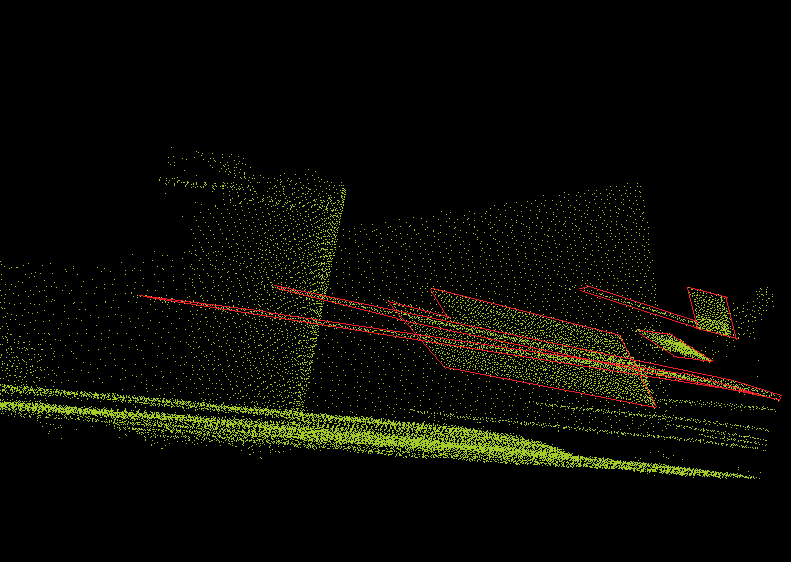
\includegraphics[width=0.9\columnwidth]{pointClouds/artefatti.png} 
    \caption{Point Cloud che presenta problemi di artefatti di un bidone conico, vista laterale}
    \label{figure:pcloud_artifacts}
\end{figure}

\subsection{Controllo di forma}
Oltre alla creazione del modello 3D e del calcolo del volume potrebbe rivelarsi molto utile per gli ispettori avere uno strumento automatico per confrontare la forma dell'oggetto ispezionato con un modello "perfetto" del bene stesso. Ad esempio potrebbe essere usato per confrontare componenti meccaniche con i loro modelli \emph{CAD} al fine di individuare eventuali deformazioni subite durante il trasporto.

\subsection{Integrazione con l'applicazione Vic}
L'azienda fornisce ai suoi dipendenti ispettori una applicazione che permette di automatizzare diverse mansioni. Tra le varie funzioni che mette a disposizione c'è quella di avviare una nuova ispezione o \emph{job} permettendo all'utente di compilare diversi \emph{form} per fornire così in tempo reale un rapporto dettagliato e standardizzato del lavoro svolto. In questo ambito una buona integrazione delle tecnologie \emph{Tango} potrebbe fornire molto valore aggiunto.


\subsection{Ricostruzione continua}
Le ricostruzioni di \emph{Samba} vengono effettuate "foto per foto", ovvero l'utente deve osservare l'oggetto da diverse angolazioni ed effettuare delle rilevazioni proprio come se si scattassero molte foto.\\
Un ottimo sviluppo sarebbe fare in modo che queste rilevazioni fossero effettuate in maniera automatica e continua, ciò darebbe molti vantaggi al sistema:
\begin{itemize}
	\item Ci sarebbero molti più dati, quindi la rilevazione sarebbe di maggiore qualità.
	\item L'applicazione sarebbe più vicina ai bisogni dell'utente.
	\item Si genererebbero molti \emph{Point Cloud} quasi uguali sovrapposti offrendo la possibilità di eliminare parte del rumore con metodi statistici (è improbabile che due scatti successivi dello stesso oggetto senza muovere il tablet siano affetti dagli stessi artefatti).
\end{itemize}
Apre però anche a nuovi problemi:
\begin{itemize}
	\item Maggiore carico di informazioni che deve essere gestito ed ottimizzato.
	\item Maggior consumo della batteria.
	\item Necessità di euristiche per determinare quale sia un \emph{Point Cloud} buono: l'utente non può più visionarli e scartare quelli affetti da errore.
\end{itemize}


\section{Problemi ancora irrisolti}

\subsection{Surriscaldamento e consumo della batteria}
Il prototipo prodotto ha un consumo della batteria piuttosto elevato ed a volte porta al surriscaldamento del dispositivo.
Ciò secondo una prima analisi è dovuto ai seguenti fattori:
\begin{itemize}
	\item Utilizzo combinato dei quattro sensori principali del \emph{device}: fotocamera a colori, fotocamera \emph{Fish-eye}\footnote{Fotocamera \emph{Fish-eye}: un obbiettivo grandangolare che abbraccia un angolo di campo di circa 180 gradi, in particolare quello in dotazione nel dispositivo usato è in bianco e nero.}, sensore \emph{IR} ed accelerometro/giroscopio. Questi sensori sono tutti necessari per il \emph{Motion Tracking} e la cattura dei \emph{Point Cloud}.
	\item Grande mole di dati da elaborare: un singolo \emph{Point Cloud} può contare anche 90 000 punti, essi devono essere elaborati e renderizzati in tempo reale.	
	\item Necessità di pesanti elaborazioni parallele: per permettere all'utente una interfaccia fluida e non rallentare i calcoli è necessario usare molti processi paralleli. Ogni scatto registrato è elaborato su di un proprio \emph{Thread} ed è presente un servizio che ottimizza ad intervalli regolari la ricostruzione corrente (indispensabile per tenere sotto controllo la complessità delle strutture dati).
	\item \emph{Rendering real-time}: come discusso in sezione \ref{cap:frame_preview} è un fondamentale requisito di usabilità avere una preview dei dati catturati dal \emph{depth sensor}. Ciò implica l'utilizzo di un \emph{render 3D} \emph{OpenGL} che richiede una grande quantità di risorse.
	\item Connessione dati: la necessità di un \emph{backend Server} comporta l'utilizzo della connessione internet. Inoltre dato il tipo di utilizzo per cui è stata ideata l'applicazione userà spesso la connessione \emph{mobile} per inviare i dati.
\end{itemize}
Risolvere queste criticità era oltre gli obiettivi dello \emph{stage}, ma è comunque stato stilato un documento contenente alcune contromisure che potranno essere usate per mitigarne gli effetti:
\begin{itemize}
	\item Effettuare le operazioni più dispendiose usando le librerie native in \emph{C} ed integrarne i risultati mediante una interfaccia \emph{Jni}.
	\item Una volta migrate le operazioni di elaborazione dei punti da \emph{Java} a \emph{C} si dovrebbero avere un sensibile incremento nelle prestazioni che permetterebbe di limitare l'elaborazione a solo due processi: uno per gestire la trasformazione dei punti (rotazione, traslazione, sovrapposizione) ed uno per le operazioni di ottimizzazione (\emph{voxeling}, rimozione rumore, rimozione ridondanze).
	\item Gestire la priorità del servizio di ottimizzazione: è trasparente all'utente e non deve necessariamente essere performante. Quindi esso può avere una minore priorità nell'utilizzo della \emph{CPU} cercando di ridurre i \emph{burst} di dati.
	\item Il \emph{render} non ha lo scopo di rappresentare tutti i punti salvati, ma di fornire all'utente una idea di quello che "vede" il sensore di profondità. Si può pensare quindi di approssimare parti della nuvola di punti a figure geometriche semplici, ad esempio il pavimento può essere approssimato ad un piano. Ciò ridurrebbe il carico di lavoro per processore e scheda grafica.
\end{itemize}
Comunque va tenuto a mente che il dispositivo è un \emph{Hardware} sperimentale che non è pensato per utilizzo su larga scala ma solo per lo sviluppo: comportamento instabile del dispositivo usando alcuni tipi di applicazioni è largamente documentato all'interno della comunità. xxxx (documentare)\\
Durante il tirocinio sono stati sperimentati questo genere di problemi anche con applicazioni rilasciate dalla \emph{Google} stessa. xxxx (documentare)

\subsection{Preview della fotocamera}
Le \emph{API} forniscono degli strumenti per automatizzare la \emph{preview} della fotocamera a colori. Essi tuttavia si sono rivelati estremamente pesanti come carico computazionale e se combinati al resto dell'applicazione prodotta possono portare a rallentamenti imprevisti.\\
Per questo si è scelto di ottenere questa anteprima tramite metodi di basso livello. Essi tuttavia richiedono uno sforzo ben maggiore e quelli applicati in \emph{Samba} vanno rivisti.\\
Un \emph{bug} noto è che alla ripresa della attività, qualche volta la \emph{preview} non viene attivata ed il riquadro a lei riservato rimane nero.


%**************************************************************
\section{Consuntivo finale}
Il periodo di \emph{stage} ha avuto avvio il 13 Giugno 2016 ed è terminato il 16 Agosto 2016 invece che il 5 Agosto. Lo slittamento della data di fine è dovuto ad impegni universitari dello studente ed a un breve periodo di chiusura estiva dell'azienda. Il tirocinio ha avuto una durata totale di 320 ore.\\
In tabella \ref{tab:preventivo-consuntivo} sono riportate le ore preventivate per ogni attività ed esse sono confrontate con le ore effettivamente impiegate.
\begin{table}[H]
	\begin{center}
	  \begin{tabular}{| l | c | c | c | c |}
	    \hline
	    \textbf{Attività} & \textbf{Preventivo} & \textbf{Consuntivo} & \textbf{Diff} & \textbf{Diff \%} \\ \hline
	    Studio preliminare & 20 & 24 & +4 & +20\%\\
	    \hline
	    Ideazione modello di soluzione & 20 & 16 & -4 & -20\%\\
	    \hline
	    Studio di fattibilità/analisi dei rischi & 20 & 32 & +12 & +60\%\\
	    \hline
	    Analisi dei requisiti & 20 & 12 & -8 & -40\%\\
	    \hline
	    Prototipi preliminari & 40 & 86 & +46 & +115\%\\
	    \hline
	    Progettazione & 40 & 30 & -10 & -25\%\\
	    \hline
	    Codifica & 120 & 80 & -40 & -33,3\%\\
	    \hline
	    Verifica e validazione & 30 & 25 & -5 & -16,6\%\\
	    \hline
	    Prove pratiche & 10 & 15 & +5 & +50\%\\
	    \hline
	    Totale & 320 & 320 & +0 & +0\%\\
	    \hline
	  \end{tabular}
	\end{center}
	\caption{Distribuzione ore preventivo e consuntivo}\label{tab:preventivo-consuntivo}
\end{table}
Le ore totali sono state rispettate e non hanno avuto variazioni.\\
La loro ripartizione interna, invece, ha subito grosse variazioni a causa di sovrastime e sottostime commesse durante la fase di pianificazione.\\
Le attività che hanno subito variazioni più importanti sono state codifica e sviluppo dei prototipi preliminari. Questi ultimi hanno richiesto più del doppio del tempo preventivato a causa della difficoltà del compito richiesto, ma soprattutto perché lo studente ha intrapreso una strada sbagliata che ha portato ad un prototipo non funzionante e che è stato interamente scartato. Si può notare però che la maggiore attenzione riposta nei prototipi preliminari ha fatto risparmiare diverse ore alla codifica: infatti molto del codice presente nei primi prototipi è stato riusato senza cambiamenti, o con modeste modifiche.\\
Anche lo studio di fattibilità ha richiesto più tempo del previsto in quanto si è rivelato necessario cercare e provare molte applicazioni, alcune delle quali non manutenute o non aggiornate.\\
In figura \ref{gantt:pianificazione} vengono riportati i diagrammi di \emph{Gantt} dove è possibile confrontare la pianificazione preventivata e quella effettiva.

\begin{figure}[H] 
    \centering 
    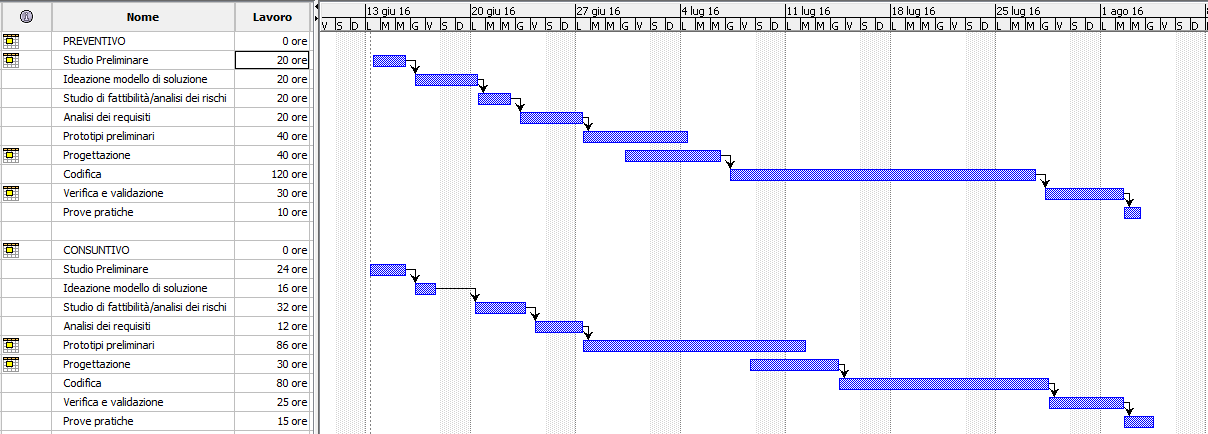
\includegraphics[width=1.0\columnwidth]{varie/ganttConsuntivo.png} 
    \caption{Gantt della pianificazione preventiva e consuntiva}
    \label{gantt:pianificazione}
\end{figure}

%**************************************************************
\section{Raggiungimento degli obiettivi}
\subsection{Obiettivi generali}
Gli obiettivi generali riportati nel piano di lavoro erano i seguenti:
\begin{itemize}
	\item Obbligatori
	\begin{itemize}
		\item \underline{\textit{ob01}}: studio delle soluzioni esistenti;
		\item \underline{\textit{ob02}}: ideazione di una soluzione per il riconoscimento di un oggetto;
		\item \underline{\textit{ob03}}: implementazione prototipo in grado di riconoscere un oggetto;
		\item \underline{\textit{ob04}}: calcolo del volume dell'oggetto (approssimato);
		\item \underline{\textit{ob05}}: implementazione app come indicato nella sezione \emph{Struttura applicazione} del documento \emph{Relazione app per Project Tango} fornito dall'azienda;
	\end{itemize}
	
	\item Desiderabili 
	\begin{itemize}
		\item \underline{\textit{de01}}: generare modello 3D in un formato portabile (obj, ply, vtk);
		\item \underline{\textit{de02}}: stima della precisione con cui viene ricostruito un oggetto;
		\item \underline{\textit{de03}}: perfezionare calcolo del volume (cavità nell'oggetto, eliminazione dati di sfondo/rumore);
		\item \underline{\textit{de04}}: stima della precisione nel calcolo del volume;
	\end{itemize}
	
	\item Opzionali
	\begin{itemize}
		\item \underline{\textit{op01}}: ottimizzazione della comunicazione con il server nel caso risultasse necessaria.
	\end{itemize} 
\end{itemize}

I requisiti obbligatori sono stati tutti raggiunti.\\
Per quanto riguarda quelli desiderabili invece:
\begin{itemize}
	\item \underline{\textit{de01}}: È stato pienamente soddisfatto.
	\item \underline{\textit{de02}}: Sono stati forniti molti modelli grafici, da cui è possibile effettuare delle considerazioni sulla precisione con cui vengono ricostruiti gli oggetti.
	\item \underline{\textit{de03}}: Non soddisfatto.
	\item \underline{\textit{de04}}: Sono stati condotti degli studi, ma si è ritenuto che l'applicazione fosse ad uno stato ancora troppo poco avanzato perché la statistica avesse senso.
\end{itemize}
Il requisito opzionale \underline{\textit{op01}} non è stato raggiunto.

\subsection{Requisiti}
Dagli obiettivi posti nel piano di lavoro sono stati ricavati i requisiti esposti nel capitolo \ref{cap:analisi-requisiti}. Seguono le tabelle di soddisfacimento di questi ultimi divisi per categorie.

\subsubsection{Requisiti funzionali}
\LTXtable{\textwidth}{tabelle/requisiti/soddisfacimento/funzionali.tex}
Segue una tabella riassuntiva di questa tipologia di requisiti.
\begin{table}[H]
	\begin{center}
	  \begin{tabular}{ l  c  c  c }
	    \hline
	    \textbf{Tipologia} & \textbf{Totali} & \textbf{Soddisfatti} & \textbf{Percentuale} \\ \hline
	    Obbligatori & 44 & 44 & 100\%\\ \hline
	    Desiderabili & 2 & 0 & 0\%\\
	    \hline
	  \end{tabular}
	\end{center}
	\caption{Tabella riassuntiva del soddisfacimento dei requisiti funzionali}
\end{table}

\subsubsection{Requisiti qualitativi}
\LTXtable{\textwidth}{tabelle/requisiti/soddisfacimento/qualitativi.tex}
Segue una tabella riassuntiva di questa tipologia di requisiti.
\begin{table}[H]
	\begin{center}
	  \begin{tabular}{ l  c  c  c }
	    \hline
	    \textbf{Tipologia} & \textbf{Totali} & \textbf{Soddisfatti} & \textbf{Percentuale} \\ \hline
	    Obbligatori & 3 & 3 & 100\%\\ \hline
	    Desiderabili & 1 & 1 & 100\%\\
	    \hline
	  \end{tabular}
	\end{center}
	\caption{Tabella riassuntiva del soddisfacimento dei requisiti qualitativi}
\end{table}

\subsubsection{Requisiti di vincolo}
\LTXtable{\textwidth}{tabelle/requisiti/soddisfacimento/vincolo.tex}
Segue una tabella riassuntiva di questa tipologia di requisiti.
\begin{table}[H]
	\begin{center}
	  \begin{tabular}{ l  c  c  c }
	    \hline
	    \textbf{Tipologia} & \textbf{Totali} & \textbf{Soddisfatti} & \textbf{Percentuale} \\ \hline
	    Obbligatori & 2 & 2 & 100\%\\
	    \hline
	  \end{tabular}
	\end{center}
\caption{Tabella riassuntiva del soddisfacimento dei requisiti di vincolo}
\end{table}	

\subsubsection{Requisiti prestazionali}
\LTXtable{\textwidth}{tabelle/requisiti/soddisfacimento/prestazionali.tex}
Segue una tabella riassuntiva di questa tipologia di requisiti.
\begin{table}[H]
	\begin{center}
	  \begin{tabular}{ l  c  c  c }
	    \hline
	    \textbf{Tipologia} & \textbf{Totali} & \textbf{Soddisfatti} & \textbf{Percentuale} \\ \hline
	    Obbligatori & 2 & 2 & 100\%\\ \hline
	    Desiderabili & 8 & 8 & 100\%\\
	    \hline
	  \end{tabular}
	\end{center}
\caption{Tabella riassuntiva del soddisfacimento dei requisiti prestazionali}
\end{table}	
Attenzione particolare è stata posta al requisito \emph{RDP-1.2}. Esso richiede che sia possibile effettuare almeno 5-6 catture al secondo. Studi sperimentali condotti in diversi ambienti confermano che le rilevazioni impiegano in media circa 220 millisecondi ad essere elaborato, quindi circa 4,5 riprese al secondo. È però possibile in ogni caso far effettuare un numero arbitrario di rilevazioni, che verranno elaborate su \emph{thread} paralleli, e anche se la loro elaborazione richiede più di un secondo è quindi possibile effettuare le 5-6 riprese a secondo richieste a patto di essere disposti ad aspettare qualche tempo per la loro elaborazione. Per questo il requisito è segnalato come parzialmente soddisfatto.


\subsubsection{Soddisfacimento requisiti}
Segue una tabella generale che riassume la copertura di tutti i requisiti.
\begin{table}[H]
	\begin{center}
	  \begin{tabular}{ l  c  c  c }
	    \hline
	    \textbf{Tipologia} & \textbf{Totali} & \textbf{Soddisfatti} & \textbf{Percentuale} \\ \hline
	    Obbligatori & 51 & 51 & 100\%\\ \hline
	    Desiderabili & 11 & 9 & 81,8\%\\
	    \hline
	  \end{tabular}
	\end{center}
\caption{Tabella riassuntiva del soddisfacimento di tutti i requisiti}
\end{table}	
%**************************************************************
\section{Conoscenze acquisite}
Dal punto di vista formativo l'attività di \emph{stage} è stata estremamente positiva. Ha arricchito il mio bagaglio personale di competenze professionali.\\

La richiesta di app \emph{mobile} è in continuo aumento. Per questo l'apprendimento della progettazione e sviluppo delle applicazioni mobili \emph{Android} è certamente una pietra miliare in campo \emph{IT} in questi anni.\\

L'approccio ad una tecnologia sperimentale ed ancora di nicchia come \emph{Tango Project} crea dei vantaggi in ambito occupazionale in quanto gli sviluppatori non sono molti. Inoltre il rilascio del primo \emph{smartphone} commerciale dotato dei sensori \emph{Tango} è stato annunciato da un noto marchio per settembre 2016; se dovesse prendere campo anche in ambito \emph{customer} ci sarebbe certamente una grande richiesta di sviluppatori con esperienza vista la scarsità di applicazioni dedicate a questo tipo di \emph{Hardware}. Altro aspetto positivo è stato l'inserimento all'interno della comunità degli sviluppatori \emph{Tango} sia su \emph{StackOverflow} che su \emph{Google plus}; lo studente ha avuto modo di confrontarsi con addetti \emph{Google} e con altri sviluppatori sia in ambito accademico/di ricerca che in ambito industriale.\\

In ambito aziendale si è usato \emph{Java} come linguaggio di programmazione ed \emph{Android Studio} come \emph{IDE}. La curva di apprendimento di questi strumenti è stata piuttosto rapida grazie all'esperienza già maturata in ambito accademico con \emph{Java} ed \emph{ItelliJ}, su cui è basato \emph{Android Studio}. Più complessa si è rivelata l'assimilazione e la comprensione del \emph{Framework Jni}, sia a causa della sua intrinseca complessità sia al fatto che \emph{Android Studio} lo supporta solo in \emph{release} sperimentale. Infatti in azienda è stato realizzato sono un piccolo prototipo che dimostra l'agibilità di questa via, ma poi la tecnologia \emph{Jni} è stata abbandonata in favore di uno sviluppo interamente in \emph{Java}. In ogni caso molte applicazioni \emph{mobile} specialmente in ambito grafico ne fanno uso, quindi ai fini del curriculum si è rivelata comunque un'esperienza fruttuosa.\\

In generale ritengo l'approccio a librerie grafiche sia \emph{mobile} che per \emph{PC} estremamente interessante ai fini della formazione personale.\\

L'apprendimento delle potenzialità della libreria \emph{PCL} e la gestione dei \emph{Point Cloud} è altrettanto importante, anche perché è uno dei pochi ambiti in cui l'Italia spicca in ambito di \emph{Computer} grafica.


%**************************************************************
%\section{Valutazione personale}







             % Conclusioni
\appendix                               
% !TEX encoding = UTF-8
% !TEX TS-program = pdflatex
% !TEX root = ../tesi.tex
% !TEX spellcheck = it-IT

%**************************************************************
\chapter{Specifica Tecnica}\label{appendix:specifica_tecnica}
%**************************************************************
\section{Metodo e formalismo di specifica}
Nell'esposizione dell'architettura del prodotto si procederà con un approccio di tipo top-down.  Si descriverà quindi l'architettura iniziando dal generale ed andando al particolare; descrivendo prima i componenti, per poi descrivere nel dettaglio le singole classi.\\
Per ogni componente saranno descritti brevemente il tipo, l'obiettivo e la funzione e saranno specificati
eventuali figli, classi ed interazioni con altri componenti. Ogni classe sarà dotata di una breve descrizione e
ne saranno specificate le responsabilità, le classi ereditate, le sottoclassi e le relazioni con altre classi.\\
Infine si illustreranno degli esempi di utilizzo dei \emph{design pattern} nell'architettura del sistema.

\section{Legenda}
Tutti i diagrammi usano la convenzione di colori descritta nella legenda in figura~\ref{fig:legenda} al fine di migliorare la leggibilità. I livelli di annidamento sono da intendere per la totale struttura dei package e non solo per il singolo schema.\\
Si noti in particolare che le classi e componenti di colore arancio rappresentano classi di librerie esterne al sistema, ma vengono talora rappresentate comunque per maggiore chiarezza.
\begin{figure}[H] 
    \centering 
    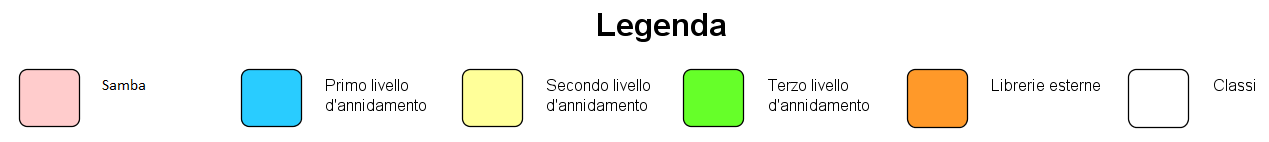
\includegraphics[width=1.0\columnwidth]{varie/Legenda.png} 
    \caption{Legenda}\label{fig:legenda}
\end{figure}

\newpage
\section{Architettura generale}
L'architettura generale è di tipo \emph{Client-Server}, la comunicazione avviene tramite semplici richieste \emph{http} e alcune notifiche vengono inviate tramite \emph{FireBase}.\\
Questo documento tuttavia esporrà solamente la parte di progettazione riguardante l'applicativo lato \emph{client}.\\
L'architettura generale della applicazione \emph{Android} è di tipo \emph{MVP} ovvero \emph{Model View Presenter}. Questo genere di architettura è stato scelto alla luce delle \emph{Android Best Practices}.\\
Il \emph{Model} contiene tutta la \emph{business logic} dell'applicazione.\\
Il \emph{Presenter} si occupa sia di osservare il modello che di aggiornare/osservare la vista. Nel caso specifico il \emph{Presenter} è composto dall'insieme delle \emph{activity} necessarie al sistema.\\
La \emph{View} è composta da \emph{file} \emph{xml} che rappresentano \emph{template} di visualizzazione e sono completamente passivi. Per questo non verranno trattati nella sezione \ref{cap:componenti-classi}.\\
Il diagramma in figura \ref{fig:arc_generale} rappresenta informalmente la struttura generale del sistema e non rispecchia la reale nomenclatura e struttura del \emph{package}.
\begin{figure}[H] 
    \centering 
    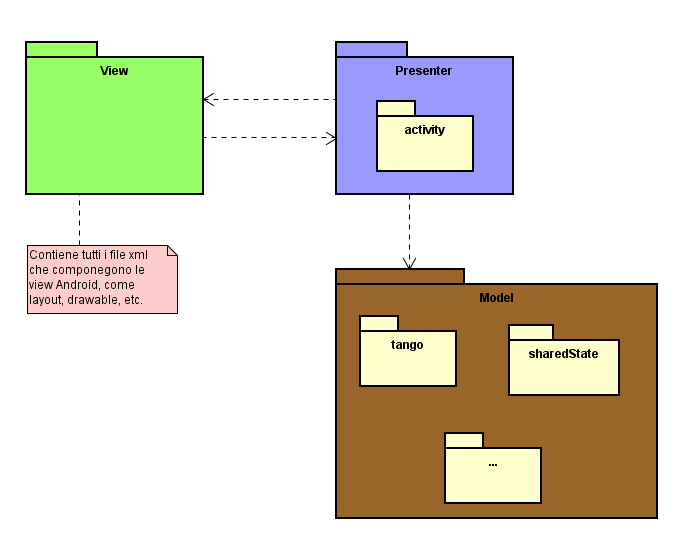
\includegraphics[width=0.9\columnwidth]{st/arc_gen_MVP.png} 
    \caption{Architettura generale del sistema}\label{fig:arc_generale}
\end{figure}



%**************************************************************
\section{Componenti e classi}\label{cap:componenti-classi}
La volontà di realizzare un prototipo ha avuto molto peso anche nella fase di progettazione. Per questo semplicità e rapidità di sviluppo sono stati obiettivi prioritari, anche sacrificando parzialmente riuso e testabilità. Ciò è stato ritenuto accettabile in quanto il prodotto non ha lo scopo di essere incrementato fino a divenire un prodotto finito, ma solo quello di essere premessa sperimentale/prototipale per un progetto futuro.\\
Di seguito viene riportata la lista delle componenti del sistema.

\subsection{Samba}\label{comp:Samba}
\begin{figure}[H] 
    \centering 
    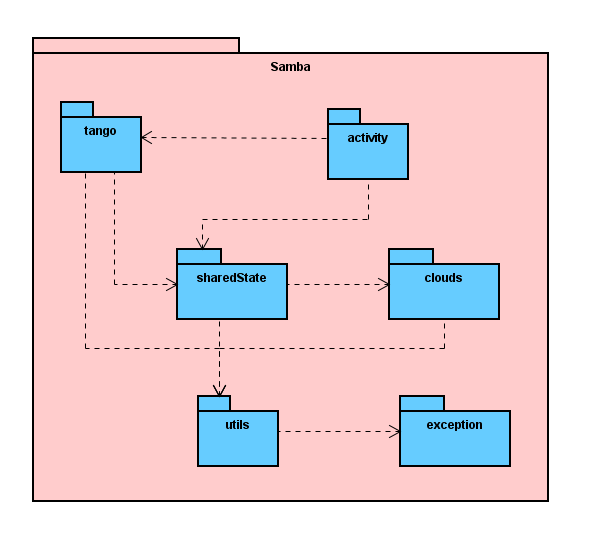
\includegraphics[width=0.9\columnwidth]{st/Samba.png} 
    \caption{Componente Samba}\label{fig:comp-Samba}
\end{figure}
\subsubsection{Descrizione}
È il livello principale del sistema lato \emph{tablet}.
\subsubsection{Package figli}
\begin{itemize}
	\item Samba.activity (\ref{comp:Samba.activity})
	\item Samba.tango (\ref{comp:Samba.tango})
	\item Samba.sharedState (\ref{comp:Samba.sharedState})
	\item Samba.clouds (\ref{comp:Samba.clouds})
	\item Samba.utils (\ref{comp:Samba.utils})
	\item Samba.exception
\end{itemize}

\newpage
\subsection{Samba.activity}\label{comp:Samba.activity}
\begin{figure}[H] 
    \centering 
    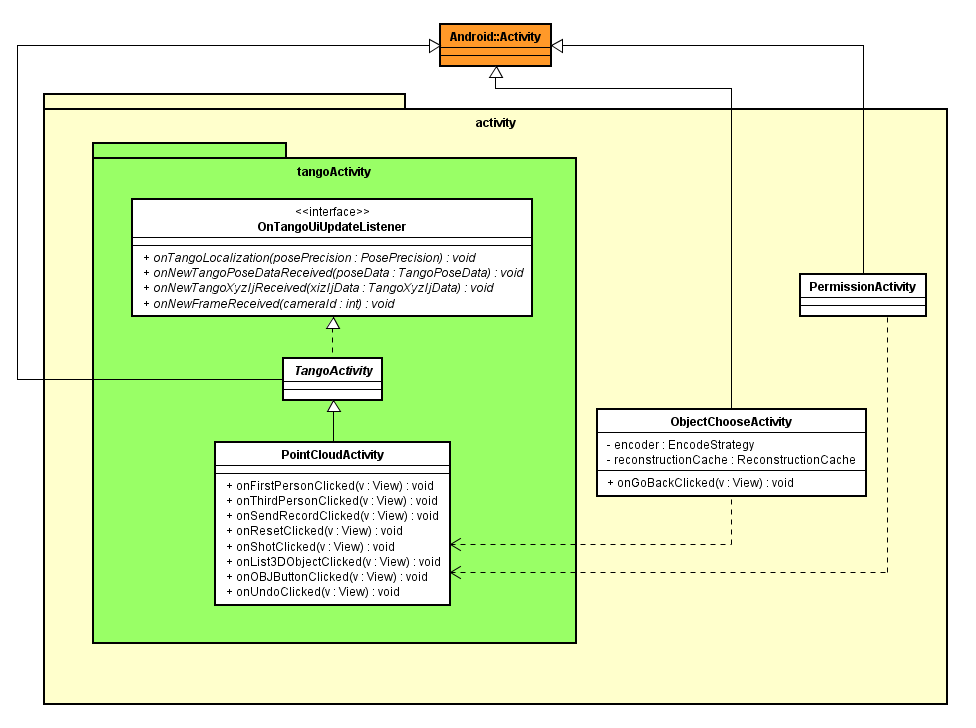
\includegraphics[width=1.0\columnwidth]{st/Samba_activity.png} 
    \caption{Componente Samba.activity}
\end{figure}
\subsubsection{Descrizione}
Questo \emph{package} contiene tutte le \emph{activity} necessarie per l'applicazione. Contiene inoltre la definizione di una interfaccia per le attività che vogliono fare uso dei vari \emph{manager} messi a disposizione (si veda sezione \ref{subs:samba-tango}).
\subsubsection{Package figli}
\begin{itemize}
	\item Samba.activity.tangoActivity (\ref{comp:Samba.activity.tangoActivity})
\end{itemize}
\subsubsection{Classi}
\begin{itemize}
	\item Samba.activity.PermissionActivity (\ref{comp:Samba.activity.PermissionActivity})
	\item Samba.activity.ObjectChooseActivity (\ref{comp:Samba.activity.ObjectChooseActivity})
\end{itemize}

\subsection{Samba.activity.tangoActivity}\label{comp:Samba.activity.tangoActivity}
\subsubsection{Descrizione}
Questo \emph{package} serve a contenere tutte le \emph{activity} che vogliono essere attività Tango, ovvero che vogliono poter usare i \emph{manager} messi a disposizione (si veda sezione \ref{subs:samba-tango}).
\subsubsection{Interfacce}
\begin{itemize}
	\item Samba.activity.tangoActivity.OnTangoUiUpdateListener (\ref{comp:Samba.activity.tangoActivity.OnTangoUiUpdateListener})
\end{itemize}
\subsubsection{Classi}
\begin{itemize}
	\item Samba.activity.tangoActivity.TangoActivity (\ref{comp:Samba.activity.tangoActivity.TangoActivity})
	\item Samba.activity.tangoActivity.PointCloudActivity (\ref{comp:Samba.activity.tangoActivity.PointCloudActivity})
\end{itemize}

\subsection{Samba.activity.tangoActivity.OnTangoUiUpdateListener}\label{comp:Samba.activity.tangoActivity.OnTangoUiUpdateListener}
\subsubsection{Descrizione}
Interfaccia che deve essere implementata da tutte le \emph{activity} che vogliono fare uso dei \emph{manager Tango} messi a disposizione (si veda sezione \ref{subs:samba-tango}). Espone metodi pubblici che possono essere chiamati da altre componenti quando avranno la necessità di notificare qualche cambiamento di stato.
\subsubsection{Utilizzo}
Viene implementate dalle \emph{activity} che vogliono interagire con il ciclo di vita dei sensori \emph{Tango}. Verrà usata per permettere indirettamente alle componenti che gestiscono i sensori \emph{Tango} di aggiornare la \emph{UI}.
\subsubsection{Implementata da}
\begin{itemize}
	\item Samba.activity.tangoActivity.TangoActivity (\ref{comp:Samba.activity.tangoActivity.TangoActivity})
\end{itemize}
\subsubsection{Relazioni con altre classi}
\begin{itemize}
 \item \texttt{Samba.clouds.utils.poseSanity.PosePrecision}: relazione uscente, dipendenza, utilizzo come parametro di uno o più metodi. (\ref{comp:Samba.clouds.utils.poseSanity.PosePrecision})
\end{itemize}

\subsection{Samba.activity.tangoActivity.TangoActivity}\label{comp:Samba.activity.tangoActivity.TangoActivity}
\subsubsection{Descrizione}
Classe astratta che estende \emph{Activity} e implementa l'interfaccia che fornisce i \emph{callback} necessari per permettere ai componenti che interagiscono con il ciclo di vita dei sensori \emph{Tango} di modificare indirettamente la \emph{UI}.
\subsubsection{Utilizzo}
È utilizzata come superclasse astratta di tutte le attività che vogliono interagire con i sensori \emph{Tango}.
\subsubsection{Relazioni con altre classi}
\begin{itemize}
	\item \texttt{Samba.sharedState.ReconstructionManager}: relazione entrante, dipendenza, utilizzo come parametro di uno o più metodi. (\ref{comp:Samba.sharedState.ReconstructionManager})
	\item \texttt{Samba.tango.CloudRecorder}: relazione entrante, dipendenza, utilizzo come parametro di uno o più metodi.(\ref{comp:Samba.tango.CloudRecorder})
	\item \texttt{Samba.tango.RajawaliRendererManager}: relazione entrante, dipendenza, utilizzo come parametro di uno o più metodi.(\ref{comp:Samba.tango.RajawaliRendererManager})
	\item \texttt{Samba.tango.RGBBoxManager}: relazione entrante, dipendenza, utilizzo come parametro di uno o più metodi.(\ref{comp:Samba.tango.RGBBoxManager})
	\item \texttt{Samba.tango.TangoManager}: relazione entrante, dipendenza, utilizzo come parametro di uno o più metodi. (\ref{comp:Samba.tango.TangoManager})
	\item \texttt{Samba.tango.RajawaliRendererManager.RajawaliRendererManager}: relazione entrante, dipendenza, utilizzo come parametro di uno o più metodi. (\ref{comp:Samba.tango.RajawaliRendererManager.RajawaliRendererManager})
\end{itemize}
\subsubsection{Estesa da}
\begin{itemize}
	\item Samba.activity.tangoActivity.PointCloudActivity (\ref{comp:Samba.activity.tangoActivity.PointCloudActivity})
\end{itemize}
\subsubsection{Interfacce implementate}
\begin{itemize}
	\item Samba.activity.tangoActivity.OnTangoUiUpdateListener (\ref{comp:Samba.activity.tangoActivity.OnTangoUiUpdateListener})
\end{itemize}
\subsubsection{Classi estese}
\begin{itemize}
	\item android.app.Activity
\end{itemize}

\subsection{Samba.activity.tangoActivity.PointCloudActivity}\label{comp:Samba.activity.tangoActivity.PointCloudActivity}
\subsubsection{Descrizione}
Attività principale dell'applicazione prodotta: fornisce un \emph{render} dei punti, una \emph{preview} della fotocamera e pulsanti per accedere a tutte le altre funzionalità dell'applicazione.\\
\subsubsection{Utilizzo}
È usata per gestire il ciclo di vita dell'\emph{activity} principale dell'applicazione.
\subsubsection{Relazioni con altre classi}
\begin{itemize}
	\item \texttt{Samba.activity.ObjectChooseActivity}: relazione entrante, dipendenza, utilizzo della classe per costruire un \emph{Intent}. (\ref{comp:Samba.activity.ObjectChooseActivity})
	\item \texttt{Samba.activity.PermissionActivity}: relazione entrante, dipendenza, utilizzo della classe per costruire un \emph{Intent}. (\ref{comp:Samba.activity.PermissionActivity})
	\item \texttt{Samba.sharedState.ReconstructionCache}: relazione uscente, composizione. (\ref{comp:Samba.sharedState.ReconstructionCache})
	\item \texttt{Samba.sharedState.ReconstructionManager}: relazione uscente, composizione.	 (\ref{comp:Samba.sharedState.ReconstructionManager})
	\item \texttt{Samba.tango.TangoManager}: relazione uscente, composizione. (\ref{comp:Samba.tango.TangoManager})
	\item \texttt{Samba.tango.RajawaliRendererManager}: relazione uscente, composizione. (\ref{comp:Samba.tango.RajawaliRendererManager})
	\item \texttt{Samba.tango.RGBBoxManager}: relazione uscente, composizione. (\ref{comp:Samba.tango.RGBBoxManager})
	\item \texttt{Samba.clouds.utils.SambaPoint}: relazione uscente, dipendenza. (\ref{comp:Samba.clouds.utils.SambaPoint})
	\item \texttt{Samba.tango.RajawaliRendererManager.RajawaliRendererManager}: relazione uscente, composizione. (\ref{comp:Samba.tango.RajawaliRendererManager.RajawaliRendererManager})
	\item \texttt{Samba.tango.CloudRecorder}: relazione uscente, composizione. (\ref{comp:Samba.tango.CloudRecorder})
\end{itemize}
\subsubsection{Classi estese}
\begin{itemize}
	\item Samba.activity.tangoActivity.TangoActivity (\ref{comp:Samba.activity.tangoActivity.TangoActivity})
\end{itemize}

\subsection{Samba.activity.ObjectChooseActivity}\label{comp:Samba.activity.ObjectChooseActivity}
\subsubsection{Descrizione}
Attività che può leggere e scrivere su disco, compila la lista dei \emph{File pcd} salvati e permette all'utente di compiere diverse azioni su questi ultimi.
\subsubsection{Utilizzo}
Viene usata quando l'utente richiede di visualizzare la lista dei \emph{file pcd} salvati su disco, oppure quando vuole caricarli/eliminarli/spedirli al \emph{Server}.
\subsubsection{Relazioni con altre classi}
\begin{itemize}
	\item \texttt{Samba.activity.tangoActivity.PointCloudActivity}: relazione uscente, dipendenza, utilizzo della classe per costruire un \emph{Intent}. (\ref{comp:Samba.activity.tangoActivity.PointCloudActivity})
	\item \texttt{Samba.clouds.utils.SambaPoint}: relazione uscente, dipendenza. (\ref{comp:Samba.clouds.utils.SambaPoint})
	\item \texttt{Samba.sharedState.ReconstructionCache} relazione uscente, composizione. (\ref{comp:Samba.sharedState.ReconstructionCache})
	\item \texttt{Samba.utils.encoding.EncodeStrategy}: relazione entrante, composizione. (\ref{comp:Samba.utils.encoding.EncodeStrategy})
\end{itemize}
\subsubsection{Classi estese}
\begin{itemize}
	\item android.app.Activity
\end{itemize}

\subsection{Samba.activity.PermissionActivity}\label{comp:Samba.activity.PermissionActivity}
\subsubsection{Descrizione}
Attività che ha il solo compito di richiedere all'utente i permessi di utilizzare l'\emph{Area Learning}. \emph{Google} fornire un \emph{Intent} apposito per ottenere tali permessi ed essi devono essere assolutamente garantiti dall'utente prima dell'inizio del processo di localizzazione. Per questo sono richiesti in una attività a parte e che viene lanciata precedentemente rispetto all'attività principale.
\subsubsection{Utilizzo}
Viene lanciata ad ogni avvio dell'applicazione allo scopo di richiedere i permessi, in caso l'utente non li abbia ancora garantiti, controllarne la presenza altrimenti.
\subsubsection{Relazioni con altre classi}
\begin{itemize}
	\item \texttt{Samba.activity.tangoActivity.PointCloudActivity}: relazione uscente, dipendenza, utilizzo della classe per costruire un \emph{Intent}. (\ref{comp:Samba.activity.tangoActivity.PointCloudActivity})
\end{itemize}
\subsubsection{Classi estese}
\begin{itemize}
	\item android.app.Activity
\end{itemize}

\newpage
\subsection{Samba.tango}\label{subs:samba-tango}
\label{comp:Samba.tango}
\begin{figure}[H] 
    \centering 
    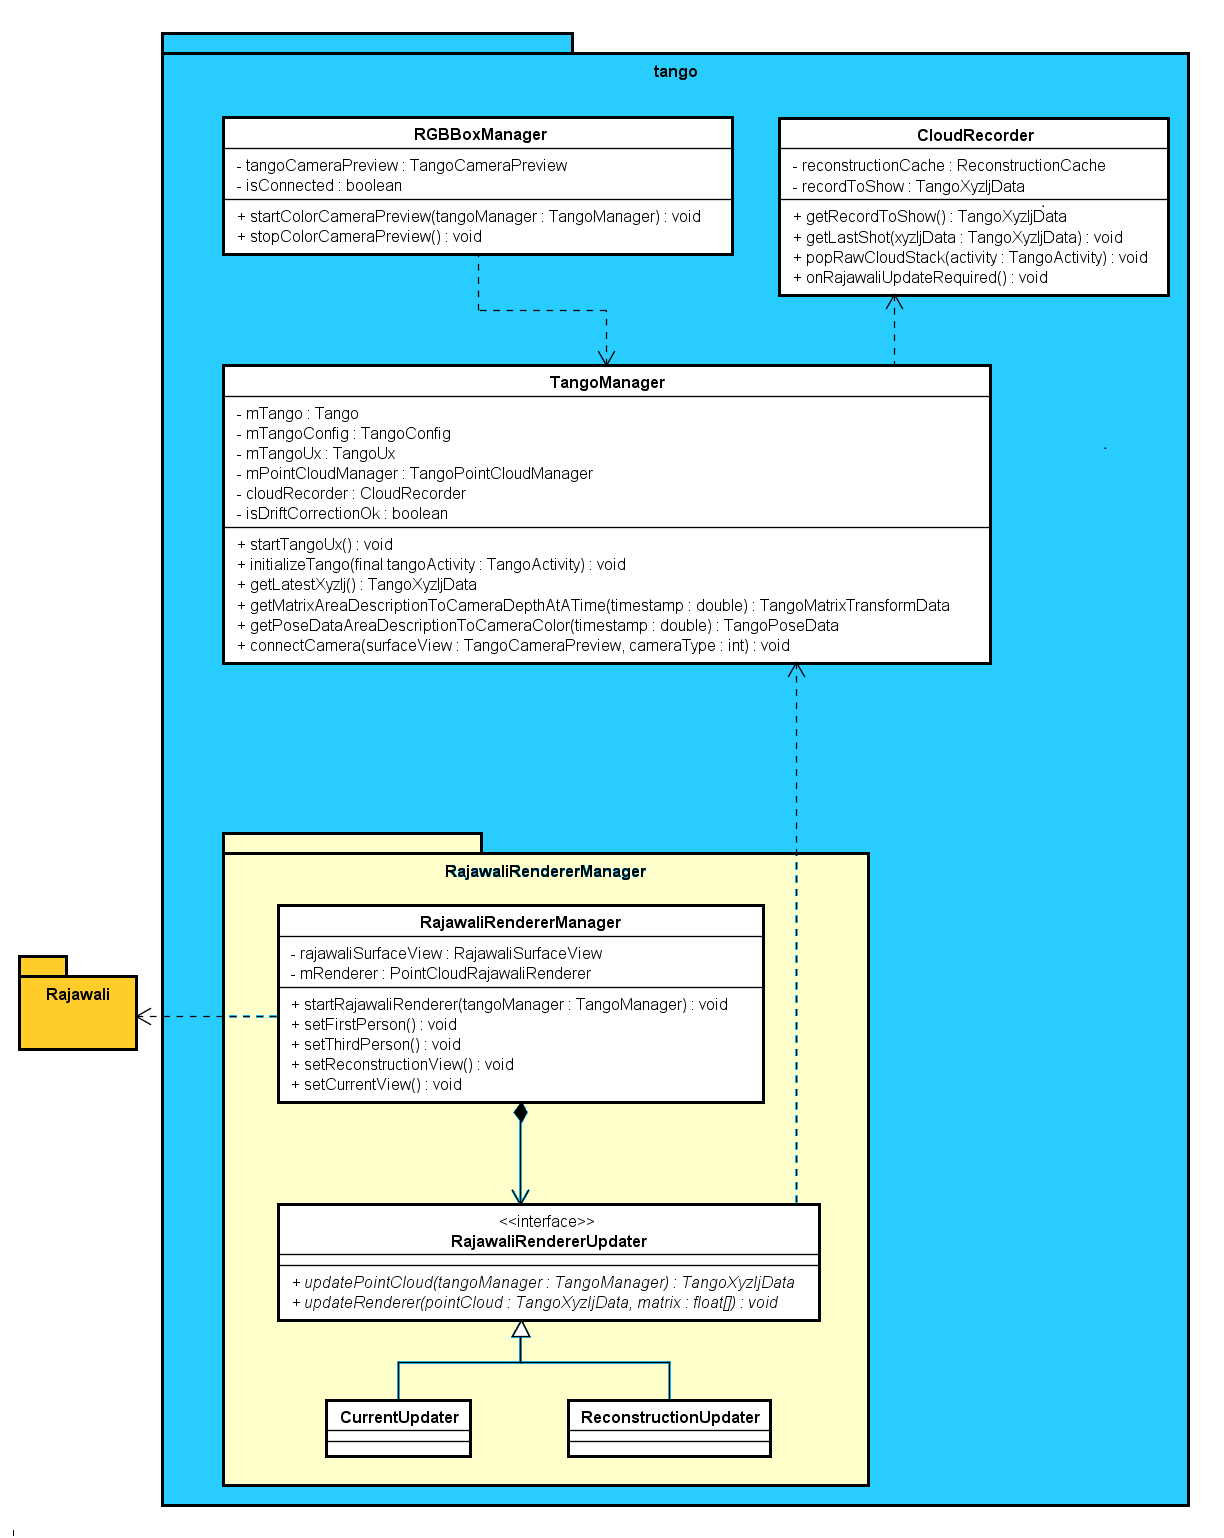
\includegraphics[width=1.1\columnwidth]{st/Samba_tango.png} 
    \caption{Componente Samba.tango}
\end{figure}
\subsubsection{Descrizione}
Questo \emph{package} contiene un insieme di classi che possono essere usate per interagire con il ciclo di vita dei sensori \emph{Tango} e del \emph{renderer} dei punti. Questi \emph{manager} possono essere usati per gestire la \emph{business logic} di una applicazione \emph{Tango} separandola dalla sua rappresentazione grafica.
\subsubsection{Package figli}
\begin{itemize}
	\item Samba.tango.RajawaliRendererManager (\ref{comp:Samba.tango.RajawaliRendererManager})
\end{itemize}
\subsubsection{Classi}
\begin{itemize}
	\item Samba.tango.RGBBoxManager (\ref{comp:Samba.tango.RGBBoxManager})
	\item Samba.tango.CloudRecorder (\ref{comp:Samba.tango.CloudRecorder})
	\item Samba.tango.TangoManager (\ref{comp:Samba.tango.TangoManager})
\end{itemize}

\subsection{Samba.tango.RajawaliRendererManager}\label{comp:Samba.tango.RajawaliRendererManager}
\subsubsection{Descrizione}
\emph{Package} che contiene il \emph{manager} per gestire il \emph{rendering} dei punti tramite la libreria \emph{Rajawali}.
\subsubsection{Interfacce}
\begin{itemize}
	\item Samba.tango.RajawaliRendererManager.RajawaliRendererUpdater (\ref{comp:Samba.tango.RajawaliRendererManager.RajawaliRendererUpdater})
\end{itemize}
\subsubsection{Classi}
\begin{itemize}
	\item Samba.tango.RajawaliRendererManager.RajawaliRendererManager (\ref{comp:Samba.tango.RajawaliRendererManager.RajawaliRendererManager})
	\item Samba.tango.RajawaliRendererManager.CurrentUpdater (\ref{comp:Samba.tango.RajawaliRendererManager.CurrentUpdater})
	\item Samba.tango.RajawaliRendererManager.ReconstructionUpdater (\ref{comp:Samba.tango.RajawaliRendererManager.ReconstructionUpdater})
\end{itemize}


\subsection{Samba.tango.RajawaliRendererManager.RajawaliRendererManager}\label{comp:Samba.tango.RajawaliRendererManager.RajawaliRendererManager}
\subsubsection{Descrizione}
Questa classe permette di integrare un servizio di \emph{rendering} di \emph{Point Cloud} all'interno del ciclo di vita di una applicazione \emph{Andorid}. Oltre alla visualizzazione espone metodi per cambiare la modalità del \emph{render}, e di effettuare qualche azione sullo stesso.
\subsubsection{Utilizzo}
È utilizzata per fornire un \emph{render} nell'attività principale dell'applicazione prodotta. (Come quello in figura \ref{fig:render-rajawali} in tutta la parte destra dello schermo)
\subsubsection{Relazioni con altre classi}
\begin{itemize}
	\item \texttt{Samba.activity.tangoActivity.PointCloudActivity}: relazione entrante, composizione. (\ref{comp:Samba.activity.tangoActivity.PointCloudActivity})
	\item \texttt{Samba.activity.tangoActivity.TangoActivity}: relazione uscente, dipendenza, utilizzo come parametro di uno o più metodi. (\ref{comp:Samba.activity.tangoActivity.TangoActivity})
	\item \texttt{Samba.tango.RajawaliRendererManager.RajawaliRendererUpdater}: relazione uscente, composizione. (\ref{comp:Samba.tango.RajawaliRendererManager.RajawaliRendererUpdater})
\end{itemize}

\subsection{Samba.tango.RajawaliRendererManager.RajawaliRendererUpdater}\label{comp:Samba.tango.RajawaliRendererManager.RajawaliRendererUpdater}
\subsubsection{Descrizione}
Interfaccia che rappresenta il componente \emph{Strategy} del \emph{Design Pattern} \emph{Strategy}.
\subsubsection{Utilizzo}
È usata per alternare la modalità del \emph{render} tra la rappresentazione in tempo reale dei dati del sensore e quella della ricostruzione corrente.
\subsubsection{Relazioni con altre classi}
\begin{itemize}
	\item \texttt{Samba.tango.RajawaliRendererManager.RajawaliRendererManager}: relazione entrante, composizione. (\ref{comp:Samba.tango.RajawaliRendererManager.RajawaliRendererManager})
	\item \texttt{Samba.tango.TangoManager}: relazione uscente, dipendenza. (\ref{comp:Samba.tango.TangoManager})
\end{itemize}
\subsubsection{Implementata da}
\begin{itemize}
	\item Samba.tango.RajawaliRendererManager.CurrentUpdater (\ref{comp:Samba.tango.RajawaliRendererManager.CurrentUpdater})
	\item Samba.tango.RajawaliRendererManager.ReconstructionUpdater (\ref{comp:Samba.tango.RajawaliRendererManager.ReconstructionUpdater})
\end{itemize}


\subsection{Samba.tango.RajawaliRendererManager.CurrentUpdater}\label{comp:Samba.tango.RajawaliRendererManager.CurrentUpdater}
\subsubsection{Descrizione}
Implementazione di \emph{RajawaliRendererUpdater} che rappresenta la visione in tempo reale dei dati del sensore.
\subsubsection{Utilizzo}
È usata per impostare il \emph{render} alla modalità in tempo reale.
\subsubsection{Interfacce implementate}
\begin{itemize}
	\item Samba.tango.RajawaliRendererManager.RajawaliRendererUpdater (\ref{comp:Samba.tango.RajawaliRendererManager.RajawaliRendererUpdater})
\end{itemize}

\subsection{Samba.tango.RajawaliRendererManager.ReconstructionUpdater}\label{comp:Samba.tango.RajawaliRendererManager.ReconstructionUpdater}
\subsubsection{Descrizione}
Implementazione di \emph{RajawaliRendererUpdater} che rappresenta la visione del \emph{Point Cloud} correntemente ricostruito.
\subsubsection{Utilizzo}
È usata per impostare il \emph{render} alla modalità ricostruzione.
\subsubsection{Interfacce implementate}
\begin{itemize}
	\item Samba.tango.RajawaliRendererManager.RajawaliRendererUpdater (\ref{comp:Samba.tango.RajawaliRendererManager.RajawaliRendererUpdater})
\end{itemize}

\subsection{Samba.tango.RGBBoxManager}\label{comp:Samba.tango.RGBBoxManager}
\subsubsection{Descrizione}
Questa classe permette di integrare un servizio di \emph{preview} della fotocamera all'interno del ciclo di vita di una applicazione \emph{Andorid}.
\subsubsection{Utilizzo}
È utilizzata per fornire una \emph{preview} della fotocamera nell'attività principale dell'applicazione prodotta. (Come quella in figura \ref{fig:render-rajawali} in basso a sinistra)
\subsubsection{Relazioni con altre classi}
\begin{itemize}
	\item \texttt{Samba.activity.tangoActivity.PointCloudActivity}: relazione entrante, composizione. (\ref{comp:Samba.activity.tangoActivity.PointCloudActivity})
	\item \texttt{Samba.activity.tangoActivity.TangoActivity}: relazione uscente, dipendenza, utilizzo come parametro di uno o più metodi. (\ref{comp:Samba.activity.tangoActivity.TangoActivity})
	\item \texttt{Samba.tango.TangoManager}: relazione uscente, dipendenza. (\ref{comp:Samba.tango.TangoManager})
\end{itemize}

\subsection{Samba.tango.TangoManager}\label{comp:Samba.tango.TangoManager}
\subsubsection{Descrizione}
Questa classe permette di integrare i servizi \emph{Tango} all'interno del ciclo di vita di una applicazione \emph{Andorid}. Inoltre imposta correttamente il \emph{framework} \emph{TangoUx} e fornisce metodi per ricavare statistiche e dati algebrici.
\subsubsection{Utilizzo}
È utilizzata per fornire all'attività principale dell'applicazione prodotta la possibilità di sfruttare i servizi \emph{Tango}.
\subsubsection{Relazioni con altre classi}
\begin{itemize}
	\item \texttt{Samba.activity.tangoActivity.PointCloudActivity}: relazione entrante, composizione. (\ref{comp:Samba.activity.tangoActivity.PointCloudActivity})
	\item \texttt{Samba.activity.tangoActivity.TangoActivity}: relazione uscente, dipendenza, utilizzo come parametro di uno o più metodi. (\ref{comp:Samba.activity.tangoActivity.TangoActivity})
	\item \texttt{Samba.tango.RGBBoxManager}: relazione entrante, dipendenza. (\ref{comp:Samba.tango.RGBBoxManager})
	\item \texttt{Samba.tango.RajawaliRendererManager.RajawaliRendererUpdater}: relazione entrante, dipendenza. (\ref{comp:Samba.tango.RajawaliRendererManager.RajawaliRendererUpdater})
	\item \texttt{Samba.tango.CloudRecorder}: relazione uscente, dipendenza. (\ref{comp:Samba.tango.CloudRecorder})
	\item \texttt{Samba.clouds.utils.poseSanity.PoseSanityChecker}: relazione uscente, composizione. (\ref{comp:Samba.clouds.utils.poseSanity.PoseSanityChecker})
	\item \texttt{Samba.clouds.utils.poseSanity.PoseDriftCorrectionStatus}: relazione uscente, dipendenza. (\ref{comp:Samba.clouds.utils.poseSanity.PoseDriftCorrectionStatus})
\end{itemize}

\subsection{Samba.tango.CloudRecorder}\label{comp:Samba.tango.CloudRecorder}
\subsubsection{Descrizione}
Mantiene la ricostruzione corrente in un formato comprensibile dal \emph{renderer}.
\subsubsection{Utilizzo}
Viene usata per effettuare il \emph{rendering} del \emph{Point Cloud} della ricostruzione corrente.
\subsubsection{Relazioni con altre classi}
\begin{itemize}
	\item \texttt{Samba.activity.tangoActivity.PointCloudActivity}: relazione entrante, composizione. (\ref{comp:Samba.activity.tangoActivity.PointCloudActivity})
	\item \texttt{Samba.activity.tangoActivity.TangoActivity}: relazione uscente, dipendenza, utilizzo come parametro di uno o più metodi. (\ref{comp:Samba.activity.tangoActivity.TangoActivity})
	\item \texttt{Samba.tango.TangoManager}: relazione entrante, dipendenza. (\ref{comp:Samba.tango.TangoManager})
	\item \texttt{Samba.sharedState.ReconstructionCache}: relazione uscente, composizione. (\ref{comp:Samba.sharedState.ReconstructionCache})
	\item \texttt{Samba.clouds.utils.SambaRawData}: relazione uscente, dipendenza. (\ref{comp:Samba.clouds.utils.SambaRawData})
	\item \texttt{Samba.utils.encoding.EncodeStrategy}: relazione uscente, composizione. (\ref{comp:Samba.utils.encoding.EncodeStrategy})
\end{itemize}


\newpage
\subsection{Samba.sharedState}\label{comp:Samba.sharedState}
\begin{figure}[H] 
    \centering 
    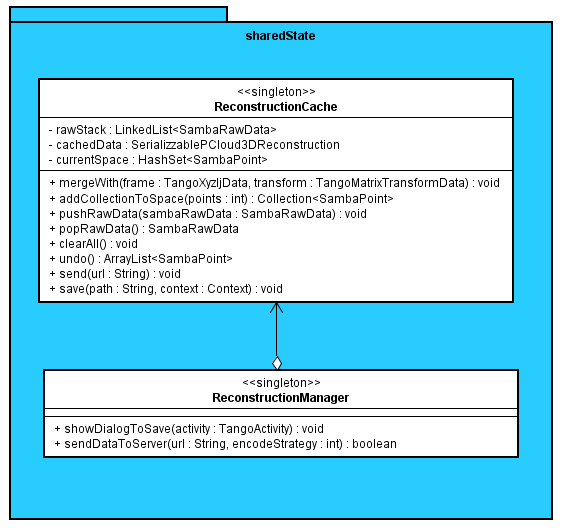
\includegraphics[width=0.9\columnwidth]{st/Samba_sharedState.png} 
    \caption{Componente Samba.sharedState}
\end{figure}
\subsubsection{Descrizione}
Questo \emph{package} contiene un \emph{singleton} che mantiene tutti gli stati condivisi tra i vari servizi e una classe di utilità.
\subsubsection{Classi}
\begin{itemize}
	\item Samba.sharedState.ReconstructionCache (\ref{comp:Samba.sharedState.ReconstructionCache})
	\item Samba.sharedState.ReconstructionManager (\ref{comp:Samba.sharedState.ReconstructionManager})
\end{itemize}

\subsection{Samba.sharedState.ReconstructionCache}\label{comp:Samba.sharedState.ReconstructionCache}
\subsubsection{Descrizione}
Questo \emph{singleton} mantiene tutte le informazioni condivise tra i vari servizi asincroni presenti nell'applicazione. Fornisce tutti i metodi necessari per accedervi controllatamente, e si occupa anche di sincronizzare gli accessi stessi dove necessario.
\subsubsection{Utilizzo}
È usata dai servizi presenti nell'applicazione per salvare e modificare i loro stati condivisi.
\subsubsection{Relazioni con altre classi}
\begin{itemize}
	\item \texttt{Samba.sharedState.ReconstructionManager}: relazione entrante, aggregazione. (\ref{comp:Samba.sharedState.ReconstructionManager})
	\item \texttt{Samba.activity.ObjectChooseActivity}: relazione entrante, composizione. (\ref{comp:Samba.activity.ObjectChooseActivity})
	\item \texttt{Samba.activity.tangoActivity.PointCloudActivity}: relazione entrante, composizione. (\ref{comp:Samba.activity.tangoActivity.PointCloudActivity})
	\item \texttt{Samba.tango.CloudRecorder}: relazione entrante, composizione. (\ref{comp:Samba.tango.CloudRecorder})
	\item \texttt{Samba.utils.services.MergingService}: relazione entrante, composizione. (\ref{comp:Samba.utils.services.MergingService})
	\item \texttt{Samba.utils.services.VoxelService}: relazione entrante, composizione.	 (\ref{comp:Samba.utils.services.VoxelService})
	\item \texttt{Samba.clouds.reconstruction.UndoableReconstruction}: relazione uscente, dipendenza, controllo di tipo. (\ref{comp:Samba.clouds.reconstruction.UndoableReconstruction})
	\item \texttt{Samba.clouds.utils.SambaPoint}: relazione uscente, dipendenza. (\ref{comp:Samba.clouds.utils.SambaPoint})
	\item \texttt{Samba.clouds.utils.SambaRawData}: relazione uscente, composizione. (\ref{comp:Samba.clouds.utils.SambaRawData})
	\item \texttt{Samba.utils.sending.ReconstructionSender}: relazione uscente, composizione. (\ref{comp:Samba.utils.sending.ReconstructionSender})
	\item \texttt{Samba.utils.sending.InternalStorageSender}: relazione uscente, composizione. (\ref{comp:Samba.utils.sending.InternalStorageSender})
	\item \texttt{Samba.utils.sending.ArrListSender}: relazione uscente, composizione.	 (\ref{comp:Samba.utils.sending.ArrListSender})
	\item \texttt{Samba.clouds.reconstruction.SerializzablePCloud3DReconstruction}: relazione uscente, composizione. (\ref{comp:Samba.clouds.reconstruction.SerializzablePCloud3DReconstruction})
\end{itemize}

\subsection{Samba.sharedState.ReconstructionManager}\label{comp:Samba.sharedState.ReconstructionManager}
\subsubsection{Descrizione}
\emph{Singleton} di utilità che fornisce delle \emph{macro} per sequenze di operazioni effettuate ricorrentemente su \emph{ReconstructionCache}.
\subsubsection{Utilizzo}
Viene usato da alcuni componenti per effettuare complesse operazioni sullo stato condiviso.
\subsubsection{Relazioni con altre classi}
\begin{itemize}
	\item \texttt{Samba.sharedState.ReconstructionCache}: relazione uscente, aggregazione. (\ref{comp:Samba.sharedState.ReconstructionCache})
	\item \texttt{Samba.activity.tangoActivity.PointCloudActivity}: relazione entrante, composizione. (\ref{comp:Samba.activity.tangoActivity.PointCloudActivity})
	\item \texttt{Samba.activity.tangoActivity.TangoActivity}: relazione uscente, dipendenza, utilizzo come parametro di uno o più metodi. (\ref{comp:Samba.activity.tangoActivity.TangoActivity})
\end{itemize}

\newpage
\subsection{Samba.clouds}\label{comp:Samba.clouds}
\begin{figure}[H] 
    \centering 
    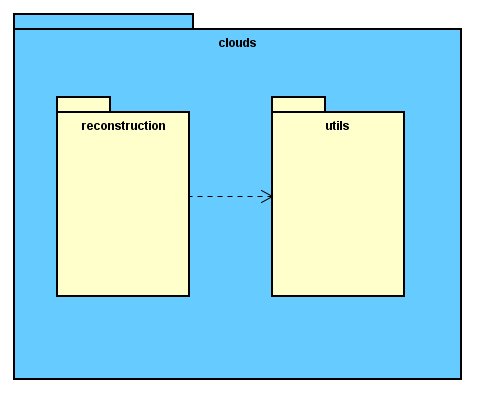
\includegraphics[width=0.8\columnwidth]{st/Samba_clouds.png} 
    \caption{Componente Samba.clouds}
\end{figure}
\subsubsection{Descrizione}
Questo \emph{package} contiene tutte le strutture dati usate per rappresentare internamente i \emph{Point Cloud}.
\subsubsection{Package figli}
\begin{itemize}
	\item Samba.clouds.reconstruction (\ref{comp:Samba.clouds.reconstruction})
	\item Samba.clouds.utils (\ref{comp:Samba.clouds.utils})
\end{itemize}

\newpage
\subsection{Samba.clouds.reconstruction}\label{comp:Samba.clouds.reconstruction}
\begin{figure}[H] 
    \centering 
    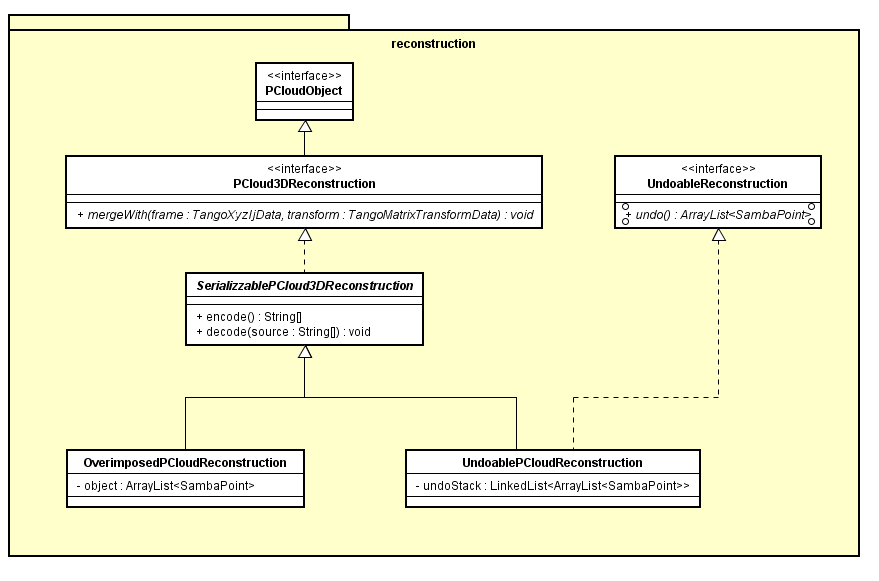
\includegraphics[width=1.0\columnwidth]{st/Samba_clouds_reconstruction.png} 
    \caption{Componente Samba.reconstruction}
\end{figure}
\subsubsection{Descrizione}
Per motivi di ottimizzazione si è cercato di lasciare il più possibile aperte le possibilità di modifica della rappresentazione interna dei \emph{Point Cloud} ricostruiti. Questo \emph{package} contiene tutte le classi che rappresenta un \emph{Point Cloud} ricostruito.
\subsubsection{Interfacce}
\begin{itemize}
	\item Samba.clouds.reconstruction.PCloudObject (\ref{comp:Samba.clouds.reconstruction.PCloudObject})
	\item Samba.clouds.reconstruction.PCloud3DReconstruction (\ref{comp:Samba.clouds.reconstruction.PCloud3DReconstruction})
	\item Samba.clouds.reconstruction.UndoableReconstruction (\ref{comp:Samba.clouds.reconstruction.UndoableReconstruction})
\end{itemize}
\subsubsection{Classi}
\begin{itemize}
	\item Samba.clouds.reconstruction.OverimposedPCloudReconstruction (\ref{comp:Samba.clouds.reconstruction.OverimposedPCloudReconstruction})
	\item Samba.clouds.reconstruction.UndoablePCloudReconstruction (\ref{comp:Samba.clouds.reconstruction.UndoablePCloudReconstruction})
\end{itemize}

\subsection{Samba.clouds.reconstruction.PCloudObject}\label{comp:Samba.clouds.reconstruction.PCloudObject}
\subsubsection{Descrizione}
Rappresenta un generico oggetto 3D rappresentato tramite \emph{Point Cloud}.
\subsubsection{Utilizzo}
È utilizzato come interfaccia alla base della gerarchia dei possibili \emph{Point Cloud}.
\subsubsection{Estesa da}
\begin{itemize}
	\item Samba.clouds.reconstruction.PCloud3DReconstruction (\ref{comp:Samba.clouds.reconstruction.PCloud3DReconstruction})
\end{itemize}

\subsection{Samba.clouds.reconstruction.PCloud3DReconstruction}\label{comp:Samba.clouds.reconstruction.PCloud3DReconstruction}
\subsubsection{Descrizione}
Interfaccia che rappresenta un generico \emph{Point Cloud} in grado di essere sovrapposto ad altre nuvole di punti per creare un oggetto tridimensionale completo.
\subsubsection{Utilizzo}
È usata come interfaccia alla base della gerarchia delle possibili ricostruzioni 3D.
\subsubsection{Interfacce estese}
\begin{itemize}
	\item Samba.clouds.reconstruction.PCloudObject (\ref{comp:Samba.clouds.reconstruction.PCloudObject})
\end{itemize}
\subsubsection{Implementata da}
\begin{itemize}
	\item Samba.clouds.reconstruction.SerializzablePCloud3DReconstruction (\ref{comp:Samba.clouds.reconstruction.SerializzablePCloud3DReconstruction})
\end{itemize}

\subsection{Samba.clouds.reconstruction.UndoableReconstruction}\label{comp:Samba.clouds.reconstruction.UndoableReconstruction}
\subsubsection{Descrizione}
Interfaccia che espone i metodi necessari per permettere ad una ricostruzione di effettuare operazioni di \emph{undo}. Una \emph{UndoableReconstruction} \textbf{non} è una \emph{PCloud3DReconstrucion}. 
\subsubsection{Utilizzo}
È implementata dalle classi che rappresentano una ricostruzione 3D e che necessitano operazioni di \emph{undo}.
\subsubsection{Relazioni con altre classi}
\begin{itemize}
	\item \texttt{Samba.sharedState.ReconstructionCache}: relazione entrante, dipendenza, controllo di tipo. (\ref{comp:Samba.sharedState.ReconstructionCache})
	\item \texttt{Samba.clouds.utils.SambaPoint}: relazione uscente, dipendenza. (\ref{comp:Samba.clouds.utils.SambaPoint})
\end{itemize}
\subsubsection{Implementata da}
\begin{itemize}
	\item Samba.clouds.reconstruction.UndoablePCloudReconstruction (\ref{comp:Samba.clouds.reconstruction.UndoablePCloudReconstruction})
\end{itemize}


\subsection{Samba.clouds.reconstruction.SerializzablePCloud3DReconstruction}\label{comp:Samba.clouds.reconstruction.SerializzablePCloud3DReconstruction}
\subsubsection{Descrizione}
Classe astratta che rappresenta un generico \emph{Point Cloud} in grado di essere sovrapposto ad altre nuvole di punti per creare un oggetto tridimensionale completo ed che può essere inoltre serializzato per salvarlo su disco o inviarlo ad un \emph{Server}.
\subsubsection{Utilizzo}
È usata come classe astratta base della gerarchia delle possibili ricostruzioni 3D.
\subsubsection{Relazioni con altre classi}
\begin{itemize}
	\item \texttt{Samba.utils.encoding.EncodeStrategy}: relazione uscente, composizione. (\ref{comp:Samba.utils.encoding.EncodeStrategy})
	\item \texttt{Samba.sharedState.ReconstructionCache}: relazione entrante, composizione. (\ref{comp:Samba.sharedState.ReconstructionCache})
	\item \texttt{Samba.utils.sending.ReconstructionSender}: relazione entrante, composizione. (\ref{comp:Samba.utils.sending.ReconstructionSender})
	\item \texttt{Samba.clouds.utils.SambaPoint}: relazione uscente, dipendenza. (\ref{comp:Samba.clouds.utils.SambaPoint})
\end{itemize}
\subsubsection{Interfacce implementate}
\begin{itemize}
	\item Samba.clouds.reconstruction.PCloud3DReconstruction (\ref{comp:Samba.clouds.reconstruction.PCloud3DReconstruction})
\end{itemize}
\subsubsection{Estesa da}
\begin{itemize}
	\item Samba.clouds.reconstruction.OverimposedPCloudReconstruction (\ref{comp:Samba.clouds.reconstruction.OverimposedPCloudReconstruction})
	\item Samba.clouds.reconstruction.UndoablePCloudReconstruction (\ref{comp:Samba.clouds.reconstruction.UndoablePCloudReconstruction})
\end{itemize}

\subsection{Samba.clouds.reconstruction.OverimposedPCloudReconstruction}\label{comp:Samba.clouds.reconstruction.OverimposedPCloudReconstruction}
\subsubsection{Descrizione}
Rappresenta una ricostruzione 3D in cui i \emph{Point Cloud} sono semplicemente sovrapposti senza alcuna ulteriore ottimizzazione.
\subsubsection{Utilizzo}
Attualmente non è usata in favore di \emph{UndoablePCloudReconstruction} (vedi \ref{class:UndoablePCloudReconstruction}).
\subsubsection{Relazioni con altre classi}
\begin{itemize}
	\item \texttt{Samba.clouds.utils.Vector4}: relazione uscente, dipendenza. (\ref{comp:Samba.clouds.utils.Vector4})
	\item \texttt{Samba.clouds.utils.SambaPoint}: relazione uscente, dipendenza. (\ref{comp:Samba.clouds.utils.SambaPoint})
\end{itemize}
\subsubsection{Classi estese}
\begin{itemize}
	\item Samba.clouds.reconstruction.SerializzablePCloud3DReconstruction (\ref{comp:Samba.clouds.reconstruction.SerializzablePCloud3DReconstruction})
\end{itemize}

\subsection{Samba.clouds.reconstruction.UndoablePCloudReconstruction}\label{comp:Samba.clouds.reconstruction.UndoablePCloudReconstruction}
\label{class:UndoablePCloudReconstruction}
\subsubsection{Descrizione}
Rappresenta una ricostruzione 3D in cui i \emph{Point Cloud} sono semplicemente sovrapposti ma con la possibilità di annullare un certo numero di operazioni.
\subsubsection{Utilizzo}
È usata come tipo preferito per contenere i dati dell'oggetto ricostruito, una volta elaborati, ma non ancora \emph{voxellati}.
\subsubsection{Relazioni con altre classi}
\begin{itemize}
	\item \texttt{Samba.clouds.utils.Vector4}: relazione uscente, dipendenza. (\ref{comp:Samba.clouds.utils.Vector4})
	\item \texttt{Samba.clouds.utils.SambaPoint}: relazione uscente, dipendenza. (\ref{comp:Samba.clouds.utils.SambaPoint})
\end{itemize}
\subsubsection{Interfacce implementate}
\begin{itemize}
	\item Samba.clouds.reconstruction.UndoableReconstruction (\ref{comp:Samba.clouds.reconstruction.UndoableReconstruction})
\end{itemize}
\subsubsection{Classi estese}
\begin{itemize}
	\item Samba.clouds.reconstruction.SerializzablePCloud3DReconstruction (\ref{comp:Samba.clouds.reconstruction.SerializzablePCloud3DReconstruction})
\end{itemize}


\newpage
\subsection{Samba.clouds.utils}\label{comp:Samba.clouds.utils}
\begin{figure}[H] 
    \centering 
    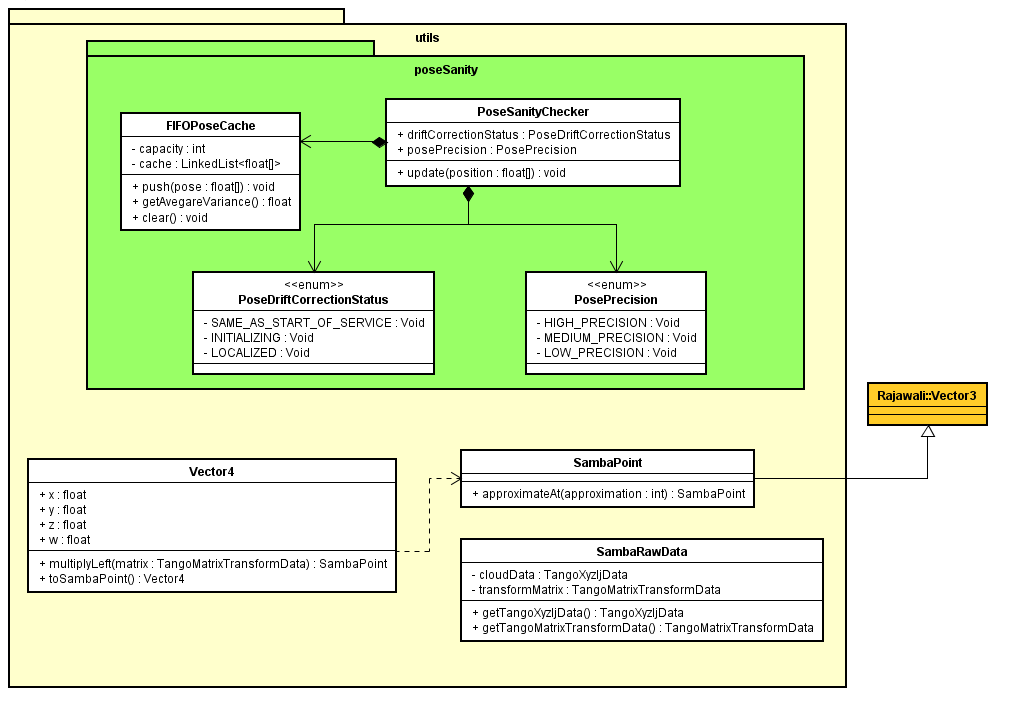
\includegraphics[width=1.2\columnwidth]{st/Samba_clouds_utils.png} 
    \caption{Componente Samba.clouds.utils}
\end{figure}
\subsubsection{Descrizione}
Contiene tutte le strutture dati di utilità usate per rappresentazione interna, come punti, \emph{Point Cloud} uniti alla propria matrice associata etc.
\subsubsection{Package figli}
\begin{itemize}
	\item Samba.clouds.utils.poseSanity (\ref{comp:Samba.clouds.utils.poseSanity})
\end{itemize}
\subsubsection{Classi}
\begin{itemize}
	\item Samba.clouds.utils.Vector4 (\ref{comp:Samba.clouds.utils.Vector4})
	\item Samba.clouds.utils.SambaPoint (\ref{comp:Samba.clouds.utils.SambaPoint})
	\item Samba.clouds.utils.SambaRawData (\ref{comp:Samba.clouds.utils.SambaRawData})
\end{itemize}

\subsection{Samba.clouds.utils.poseSanity} \label{comp:Samba.clouds.utils.poseSanity}
\subsubsection{Descrizione}
Questo \emph{package} contiene le classi necessarie per effettuare il \emph{sanity check} della fase di localizzazione.
\subsubsection{Classi}
\begin{itemize}
	\item Samba.clouds.utils.poseSanity.PoseSanityChecker (\ref{comp:Samba.clouds.utils.poseSanity.PoseSanityChecker})
	\item Samba.clouds.utils.poseSanity.FIFOPoseCache (\ref{comp:Samba.clouds.utils.poseSanity.FIFOPoseCache})
\end{itemize}
\subsubsection{Enumerazioni}
\begin{itemize}
	\item Samba.clouds.utils.poseSanity.PoseDriftCorrectionStatus (\ref{comp:Samba.clouds.utils.poseSanity.PoseDriftCorrectionStatus})
	\item Samba.clouds.utils.poseSanity.PosePrecision (\ref{comp:Samba.clouds.utils.poseSanity.PosePrecision})
\end{itemize}

\subsection{Samba.clouds.utils.poseSanity.PoseSanityChecker} \label{comp:Samba.clouds.utils.poseSanity.PoseSanityChecker}
\label{class:PoseSanityChecker}
\subsubsection{Descrizione}
Questa classe fornisce un \emph{sanity check} della fase di localizzazione.
\subsubsection{Utilizzo}
È utilizzata durante la fase di localizzazione per tenere traccia dello stato della stessa. Inoltre è usata per fornire una stima di quanto la localizzazione stessa sia avvenuta in maniera precisa.
\subsubsection{Relazioni con altre classi}
\begin{itemize}
	\item \texttt{Samba.clouds.utils.poseSanity.FIFOPoseCache}: relazione uscente, composizione. (\ref{comp:Samba.clouds.utils.poseSanity.FIFOPoseCache})
	\item \texttt{Samba.clouds.utils.poseSanity.PoseDriftCorrectionStatus}: relazione uscente, composizione. (\ref{comp:Samba.clouds.utils.poseSanity.PoseDriftCorrectionStatus})
	\item \texttt{Samba.clouds.utils.poseSanity.PosePrecision}: relazione uscente, composizione. (\ref{comp:Samba.clouds.utils.poseSanity.PosePrecision})
	\item \texttt{Samba.tango.TangoManager}: relazione entrante, composizione. (\ref{comp:Samba.tango.TangoManager})
\end{itemize}

\subsection{Samba.clouds.utils.poseSanity.FIFOPoseCache}\label{comp:Samba.clouds.utils.poseSanity.FIFOPoseCache}
\subsubsection{Descrizione}
Fornisce una cosa \emph{FIFO} in grado di tenere in memoria le ultime $n$ posizioni rilevate e usarle per dei calcoli statistici in maniera efficiente.
\subsubsection{Utilizzo}
È usata come classe di utilità per \texttt{PoseSanityChecker} (\ref{class:PoseSanityChecker}).
\subsubsection{Relazioni con altre classi}
\begin{itemize}
	\item \texttt{Samba.clouds.utils.poseSanity.PoseSanityChecker}: relazione entrante, composizione. (\ref{comp:Samba.clouds.utils.poseSanity.PoseSanityChecker})
\end{itemize}

\subsection{Samba.clouds.utils.poseSanity.PoseDriftCorrectionStatus}\label{comp:Samba.clouds.utils.poseSanity.PoseDriftCorrectionStatus}
\subsubsection{Descrizione}
Enumerazione che rappresenta i possibili stati della \emph{Drift Correction}, quelli discussi in \ref{cap:istruzioni-per-utente} alla voce "Istruzioni per l'utente".
\subsubsection{Valori}
\begin{itemize}
	\item \texttt{SAME\_AS\_START\_OF\_SERVICE}
	\item \texttt{INITIALIZING}
	\item \texttt{LOCALIZED}		
\end{itemize}
\subsubsection{Relazioni con altre classi}
\begin{itemize}
	\item \texttt{Samba.clouds.utils.poseSanity.PoseSanityChecker}: relazione entrante, composizione. (\ref{comp:Samba.clouds.utils.poseSanity.PoseSanityChecker})
	\item \texttt{Samba.tango.TangoManager}: relazione entrante, dipendenza. (\ref{comp:Samba.tango.TangoManager})
\end{itemize}


\subsection{Samba.clouds.utils.poseSanity.PosePrecision}\label{comp:Samba.clouds.utils.poseSanity.PosePrecision}
\subsubsection{Descrizione}
Enumerazione che rappresenta i possibili livelli di precisione a cui è avvenuta la localizzazione.
\subsubsection{Valori}
\begin{itemize}
	\item \texttt{HIGH\_PRECISION}
	\item \texttt{MEDIUM\_PRECISION}
	\item \texttt{LOW\_PRECISION}		
\end{itemize}
\subsubsection{Relazioni con altre classi}
\begin{itemize}
	\item \texttt{Samba.clouds.utils.poseSanity.PoseSanityChecker}: relazione entrante, composizione. (\ref{comp:Samba.clouds.utils.poseSanity.PoseSanityChecker})
	\item \texttt{Samba.activity.tangoActivity.OnTangoUiUpdateListener}: relazione entrante, dipendenza, utilizzo come parametro di uno o più metodi. (\ref{comp:Samba.activity.tangoActivity.OnTangoUiUpdateListener})
\end{itemize}

\subsection{Samba.clouds.utils.Vector4}\label{comp:Samba.clouds.utils.Vector4}
\subsubsection{Descrizione}
Classe che rappresenta un vettore di quattro dimensioni. Offre i metodi necessari per i calcoli del sistema.
\subsubsection{Utilizzo}
È usato per adattare l'interfaccia di un vettore a tre dimensioni quando è necessario moltiplicarlo per una matrice di trasformazione di un \emph{Point Cloud} (che ha quattro dimensioni).
\subsubsection{Relazioni con altre classi}
\begin{itemize}
	\item \texttt{Samba.clouds.utils.SambaPoint}: relazione uscente, dipendenza, utilizzo come parametro di uno o più metodi. (\ref{comp:Samba.clouds.utils.SambaPoint})
	\item \texttt{Samba.clouds.reconstruction.OverimposedPCloudReconstruction}: relazione entrante, dipendenza. (\ref{comp:Samba.clouds.reconstruction.OverimposedPCloudReconstruction})
	\item \texttt{Samba.clouds.reconstruction.UndoablePCloudReconstruction}: relazione entrante, dipendenza.	 (\ref{comp:Samba.clouds.reconstruction.UndoablePCloudReconstruction})
\end{itemize}

\subsection{Samba.clouds.utils.SambaPoint}\label{comp:Samba.clouds.utils.SambaPoint}
\subsubsection{Descrizione}
Questa classe rappresenta un punto all'interno di un \emph{PointCloud}. È un \emph{wrapper} di \texttt{Vector3} della libreria \emph{Rajawali}. Espone quindi le stesse funzionalità ma ne aggiunge altre di indispensabili, come essere confrontabile ed essere \emph{parcellabile}. È stato scelto di creare questo \emph{wrapper} proprio perché \texttt{Vector3} non forniva queste caratteristiche.
\subsubsection{Utilizzo}
È utilizzata ovunque sia richiesto il concetto di \emph{punto} all'interno del sistema.
\subsubsection{Relazioni con altre classi}
\begin{itemize}
	\item \texttt{Samba.clouds.utils.Vector4}: relazione entrante, dipendenza. (\ref{comp:Samba.clouds.utils.Vector4})
	\item \texttt{Samba.activity.ObjectChooseActivity}: relazione entrante, dipendenza. (\ref{comp:Samba.activity.ObjectChooseActivity})
	\item \texttt{Samba.activity.tangoActivity.PointCloudActivity}:	relazione entrante, dipendenza. (\ref{comp:Samba.activity.tangoActivity.PointCloudActivity})
	\item \texttt{Samba.clouds.reconstruction.UndoableReconstruction}: relazione entrante, dipendenza. (\ref{comp:Samba.clouds.reconstruction.UndoableReconstruction})
	\item \texttt{Samba.clouds.reconstruction.SerializzablePCloud3DReconstruction}: relazione entrante, dipendenza. (\ref{comp:Samba.clouds.reconstruction.SerializzablePCloud3DReconstruction})
	\item \texttt{Samba.clouds.reconstruction.OverimposedPCloudReconstruction}: relazione entrante, dipendenza. (\ref{comp:Samba.clouds.reconstruction.OverimposedPCloudReconstruction})
	\item \texttt{Samba.clouds.reconstruction.UndoablePCloudReconstruction}: relazione entrante, dipendenza. (\ref{comp:Samba.clouds.reconstruction.UndoablePCloudReconstruction})
	\item \texttt{Samba.sharedState.ReconstructionCache}: relazione entrante, dipendenza. (\ref{comp:Samba.sharedState.ReconstructionCache})
	\item \texttt{Samba.utils.encoding.EncodeStrategy}: relazione entrante, dipendenza. (\ref{comp:Samba.utils.encoding.EncodeStrategy})
	\item \texttt{Samba.utils.encoding.XyzEncoder}: relazione entrante, dipendenza. (\ref{comp:Samba.utils.encoding.XyzEncoder})
	\item \texttt{Samba.utils.encoding.PcdEncoder}: relazione entrante, dipendenza. (\ref{comp:Samba.utils.encoding.PcdEncoder})
	\item \texttt{Samba.utils.sending.ArrListSender}: relazione entrante, dipendenza. (\ref{comp:Samba.utils.sending.ArrListSender})
	\item \texttt{Samba.utils.sending.InternalStorageSender}: relazione entrante, dipendenza. (\ref{comp:Samba.utils.sending.InternalStorageSender})
	\item \texttt{Samba.utils.services.VoxelService}: relazione entrante, dipendenza. (\ref{comp:Samba.utils.services.VoxelService})
\end{itemize}
\subsubsection{Classi estese}
\begin{itemize}
	\item org.rajawali3d.math.vector.Vector3
\end{itemize}

\subsection{Samba.clouds.utils.SambaRawData}\label{comp:Samba.clouds.utils.SambaRawData}
\subsubsection{Descrizione}
Classe che permette di impacchettare assieme un \texttt{TangoXyzIjData} (dati del sensore di profondità \emph{Tango}) e la sua matrice di rotazione.
\subsubsection{Utilizzo}
È usata ovunque ci sia bisogno di mantenere dei dati "grezzi" prima di effettuare rotazione e traslazione.
\subsubsection{Relazioni con altre classi}
\begin{itemize}
	\item \texttt{Samba.sharedState.ReconstructionCache}: relazione entrante, composizione. (\ref{comp:Samba.sharedState.ReconstructionCache})
	\item \texttt{Samba.tango.CloudRecorder}: relazione entrante, dipendenza, utilizzo come parametro di uno o più metodi. (\ref{comp:Samba.tango.CloudRecorder})
	\item \texttt{Samba.utils.services.MergingService}: relazione entrante, dipendenza, utilizzo interno ad un metodo.	 (\ref{comp:Samba.utils.services.MergingService})
	\item \texttt{Samba.sharedState.ReconstructionCache}: relazione entrante, dipendenza. (\ref{comp:Samba.sharedState.ReconstructionCache})
\end{itemize}


\newpage
\subsection{Samba.utils}\label{comp:Samba.utils}
\begin{figure}[H] 
    \centering 
    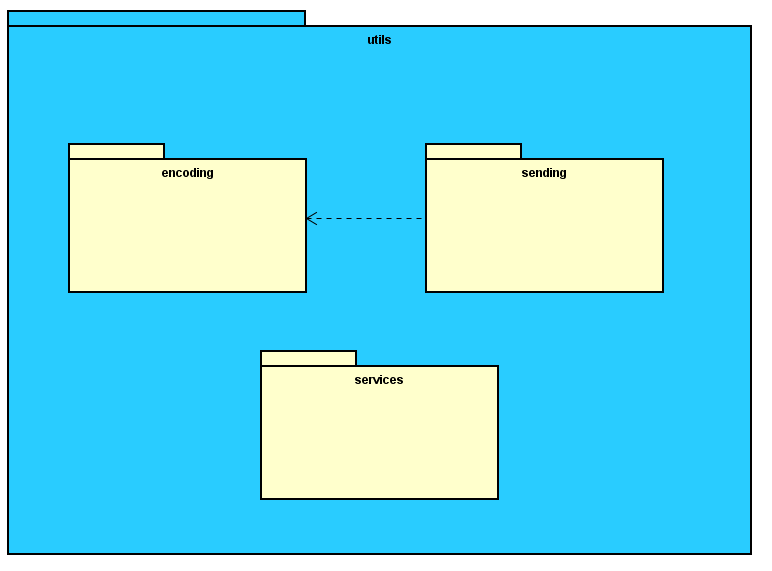
\includegraphics[width=0.9\columnwidth]{st/Samba_utils.png} 
    \caption{Componente Samba.utils}
\end{figure}
\subsubsection{Descrizione}
Questo \emph{package} contiene classi di utilità generale.
\subsubsection{Package figli}
\begin{itemize}
	\item Samba.utils.encoding (\ref{comp:Samba.utils.encoding})
	\item Samba.utils.sending (\ref{comp:Samba.utils.sending})
	\item Samba.utils.services (\ref{comp:Samba.utils.services})
\end{itemize}


\newpage
\subsection{Samba.utils.encoding}\label{comp:Samba.utils.encoding}
\begin{figure}[H] 
    \centering 
    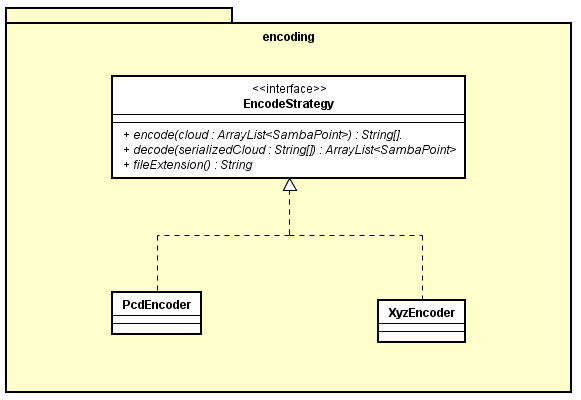
\includegraphics[width=1.0\columnwidth]{st/Samba_utils_encoding.png} 
    \caption{Componente Samba.utils.encoding}
\end{figure}
\subsubsection{Descrizione}
Questo \emph{package} contiene le classi necessarie serializzare e deserializzare i \emph{Point Cloud}.
\subsubsection{Interfacce}
\begin{itemize}
	\item Samba.utils.encoding.EncodeStrategy (\ref{comp:Samba.utils.encoding.EncodeStrategy})
\end{itemize}
\subsubsection{Classi}
\begin{itemize}
	\item Samba.utils.encoding.PcdEncoder (\ref{comp:Samba.utils.encoding.PcdEncoder})
	\item Samba.utils.encoding.XyzEncoder (\ref{comp:Samba.utils.encoding.XyzEncoder})  
\end{itemize}

\subsection{Samba.utils.encoding.EncodeStrategy}\label{comp:Samba.utils.encoding.EncodeStrategy}
\subsubsection{Descrizione}
Interfaccia che rappresenta la strategia con cui effettuare l'\emph{encoding} di un \emph{Point Cloud}.
\subsubsection{Utilizzo}
È usata come componente \emph{Strategy} di uno \emph{Strategy Pattern}.
\subsubsection{Relazioni con altre classi}
\begin{itemize}
	\item \texttt{Samba.activity.ObjectChooseActivity}: relazione entrante, composizione.   (\ref{comp:Samba.activity.ObjectChooseActivity})
	\item \texttt{Samba.clouds.reconstruction.SerializzablePCloud3DReconstruction}: relazione entrante, composizione.  (\ref{comp:Samba.clouds.reconstruction.SerializzablePCloud3DReconstruction})
	\item \texttt{Samba.utils.sending.ArrListSender}: relazione entrante, composizione. (\ref{comp:Samba.utils.sending.ArrListSender})
	\item \texttt{Samba.utils.sending.ReconstructionSender}: relazione entrante, composizione.	 (\ref{comp:Samba.utils.sending.ReconstructionSender})
	\item \texttt{Samba.utils.sending.InternalStorageSender}: relazione entrante, composizione.	 (\ref{comp:Samba.utils.sending.InternalStorageSender})
	\item \texttt{Samba.clouds.utils.SambaPoint}: relazione uscente, dipendenza, utilizzo come parametro di uno o più metodi. (\ref{comp:Samba.clouds.utils.SambaPoint})
\end{itemize}
\subsubsection{Implementata da}
\begin{itemize}
	\item Samba.utils.encoding.PcdEncoder (\ref{comp:Samba.utils.encoding.PcdEncoder})
	\item Samba.utils.encoding.XyzEncoder (\ref{comp:Samba.utils.encoding.XyzEncoder})
\end{itemize}

\subsection{Samba.utils.encoding.PcdEncoder}\label{comp:Samba.utils.encoding.PcdEncoder}
\subsubsection{Descrizione}
Implementazione della strategia di \emph{encoding} che serializza i \emph{Point Cloud} in formato \emph{pcd}.
\subsubsection{Utilizzo}
È il formato preferito dal sistema per salvare e spedire i \emph{file}.
\subsubsection{Interfacce implementate}
\begin{itemize}
	\item Samba.utils.encoding.EncodeStrategy (\ref{comp:Samba.utils.encoding.EncodeStrategy})
\end{itemize}
\subsubsection{Relazioni con altre classi}
\begin{itemize}
	\item \texttt{Samba.clouds.utils.SambaPoint}: relazione uscente, dipendenza, utilizzo come parametro di uno o più metodi. (\ref{comp:Samba.clouds.utils.SambaPoint})
\end{itemize}

\subsection{Samba.utils.encoding.XyzEncoder}\label{comp:Samba.utils.encoding.XyzEncoder}
\subsubsection{Descrizione}
Implementazione della strategia di \emph{encoding} che serializza i \emph{Point Cloud} in formato \emph{xyz}.
\subsubsection{Utilizzo}
È un formato non utilizzato nel sistema.
\subsubsection{Interfacce implementate}
\begin{itemize}
	\item Samba.utils.encoding.EncodeStrategy (\ref{comp:Samba.utils.encoding.EncodeStrategy})
\end{itemize}
\subsubsection{Relazioni con altre classi}
\begin{itemize}
	\item \texttt{Samba.clouds.utils.SambaPoint}: relazione uscente, dipendenza, utilizzo come parametro di uno o più metodi. (\ref{comp:Samba.clouds.utils.SambaPoint})
\end{itemize}


\newpage
\subsection{Samba.utils.sending}\label{comp:Samba.utils.sending}
\begin{figure}[H] 
    \centering 
    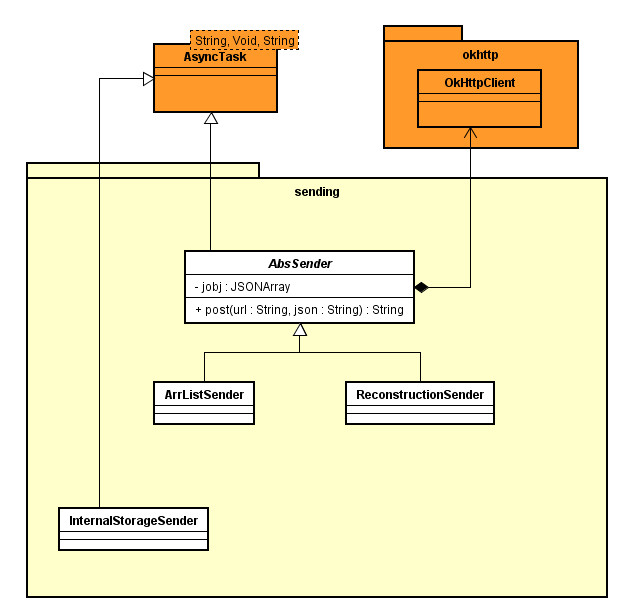
\includegraphics[width=1.0\columnwidth]{st/Samba_utils_sending.png} 
    \caption{Componente Samba.utils.sending}
\end{figure}
\subsubsection{Descrizione}
Questo \emph{package} contiene delle \emph{AsyncTask} che hanno il compito di spedire un \emph{Point Cloud} serializzato ad un \emph{Server} oppure di salvarlo su disco.
\subsubsection{Classi}
\begin{itemize}
	\item Samba.utils.sending.AbsSender (\ref{comp:Samba.utils.sending.AbsSender})
	\item Samba.utils.sending.ArrListSender (\ref{comp:Samba.utils.sending.ArrListSender})
	\item Samba.utils.sending.ReconstructionSender (\ref{comp:Samba.utils.sending.ReconstructionSender})
	\item Samba.utils.sending.InternalStorageSender (\ref{comp:Samba.utils.sending.InternalStorageSender})
\end{itemize}

\subsection{Samba.utils.sending.AbsSender}\label{comp:Samba.utils.sending.AbsSender}
\subsubsection{Descrizione}
Classe astratta per inviare un \emph{Point Cloud} tramite \emph{http} in un \emph{thread} separato dal resto dell'applicazione.
\subsubsection{Classi estese}
\begin{itemize}
	\item android.os.AsyncTask
\end{itemize}
\subsubsection{Estesa da}
\begin{itemize}
	\item Samba.utils.sending.ArrListSender (\ref{comp:Samba.utils.sending.ArrListSender})
	\item Samba.utils.sending.ReconstructionSender (\ref{comp:Samba.utils.sending.ReconstructionSender})
\end{itemize}

\subsection{Samba.utils.sending.ArrListSender}\label{comp:Samba.utils.sending.ArrListSender}
\subsubsection{Descrizione}
Classe in grado di inviare liste di \texttt{SambaPoint}.
\subsubsection{Utilizzo}
È usata per inviare liste di \texttt{SambaPoint}.
\subsubsection{Relazioni con altre classi}
\begin{itemize}
	\item \texttt{Samba.clouds.utils.SambaPoint}: relazione uscente, dipendenza. (\ref{comp:Samba.clouds.utils.SambaPoint})
	\item \texttt{Samba.utils.encoding.EncodeStrategy}: relazione uscente, composizione. (\ref{comp:Samba.utils.encoding.EncodeStrategy})
	\item \texttt{Samba.sharedState.ReconstructionCache}: relazione entrante, composizione. (\ref{comp:Samba.sharedState.ReconstructionCache})
\end{itemize}
\subsubsection{Classi estese}
\begin{itemize}
	\item Samba.utils.sending.AbsSender (\ref{comp:Samba.utils.sending.AbsSender})
\end{itemize}

\subsection{Samba.utils.sending.ReconstructionSender}\label{comp:Samba.utils.sending.ReconstructionSender}
\subsubsection{Descrizione}
Classe in grado di inviare ricostruzioni 3D.
\subsubsection{Utilizzo}
È usata per inviare ricostruzioni 3D.
\subsubsection{Relazioni con altre classi}
\begin{itemize}
	\item \texttt{Samba.clouds.utils.SambaPoint}: relazione uscente, dipendenza. (\ref{comp:Samba.clouds.utils.SambaPoint})
	\item \texttt{Samba.utils.encoding.EncodeStrategy}: relazione uscente, composizione. (\ref{comp:Samba.utils.encoding.EncodeStrategy})
	\item \texttt{Samba.sharedState.ReconstructionCache}: relazione entrante, composizione. (\ref{comp:Samba.sharedState.ReconstructionCache})
	\item \texttt{Samba.clouds.reconstruction.SerializzablePCloud3DReconstruction}: relazione uscente, composizione. (\ref{comp:Samba.clouds.reconstruction.SerializzablePCloud3DReconstruction})
\end{itemize}
\subsubsection{Classi estese}
\begin{itemize}
	\item Samba.utils.sending.AbsSender (\ref{comp:Samba.utils.sending.AbsSender})
\end{itemize}

\subsection{Samba.utils.sending.InternalStorageSender}\label{comp:Samba.utils.sending.InternalStorageSender}
\subsubsection{Descrizione}
Classe in grado di salvare su disco \emph{Point Cloud} serializzati.
\subsubsection{Utilizzo}
È usata per salvare su disco \emph{Point Cloud} serializzati.
\subsubsection{Relazioni con altre classi}
\begin{itemize}
	\item \texttt{Samba.clouds.utils.SambaPoint}: relazione uscente, dipendenza. (\ref{comp:Samba.clouds.utils.SambaPoint})
	\item \texttt{Samba.utils.encoding.EncodeStrategy}: relazione uscente, composizione. (\ref{comp:Samba.utils.encoding.EncodeStrategy})
	\item \texttt{Samba.sharedState.ReconstructionCache}: relazione entrante, composizione. (\ref{comp:Samba.sharedState.ReconstructionCache})
\end{itemize}

\newpage
\subsection{Samba.utils.services}\label{comp:Samba.utils.services}
\begin{figure}[H] 
    \centering 
    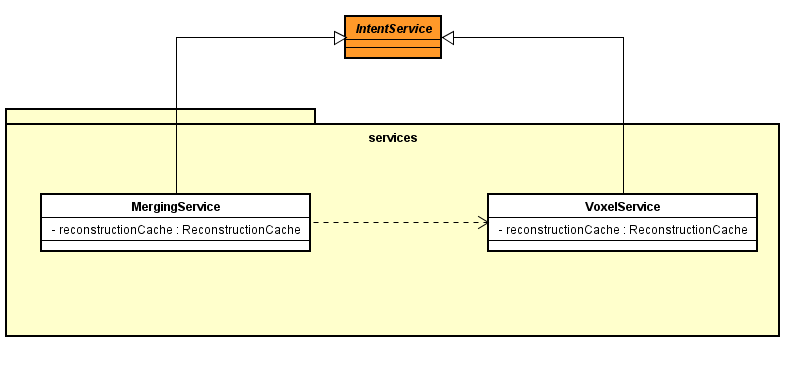
\includegraphics[width=1.0\columnwidth]{st/Samba_utils_services.png} 
    \caption{Componente Samba.utils.services}
\end{figure}
\subsubsection{Descrizione}
Questo \emph{package} contiene i servizi asincroni che servono ad effettuare operazioni sui dati raccolti dai sensori \emph{Tango}.
\subsubsection{Classi}
\begin{itemize}
	\item Samba.utils.services.MergingService (\ref{comp:Samba.utils.services.MergingService})
	\item Samba.utils.services.VoxelService (\ref{comp:Samba.utils.services.VoxelService})
\end{itemize}

\subsection{Samba.utils.services.MergingService}\label{comp:Samba.utils.services.MergingService}
\subsubsection{Descrizione}
Servizio in grado di sovrapporre ad una ricostruzione data un \emph{Point Cloud} a patto che assieme a quest'ultimo venga fornita anche la sua matrice di trasformazione.
\subsubsection{Utilizzo}
È usato per ricostruire in \emph{background} l'oggetto inquadrato dall'utente.
\subsubsection{Relazioni con altre classi}
\begin{itemize}
	\item \texttt{Samba.clouds.utils.SambaRawData}: relazione uscente, dipendenza, utilizzo interno ad un metodo. (\ref{comp:Samba.clouds.utils.SambaRawData})
	\item \texttt{Samba.utils.services.VoxelService}: relazione uscente, dipendenza. (\ref{comp:Samba.utils.services.VoxelService})
	\item \texttt{Samba.sharedState.ReconstructionCache} relazione uscente, composizione. (\ref{comp:Samba.sharedState.ReconstructionCache})
\end{itemize}
\subsubsection{Classi estese}
\begin{itemize}
	\item android.app.IntentService
\end{itemize}

\subsection{Samba.utils.services.VoxelService}\label{comp:Samba.utils.services.VoxelService}
\subsubsection{Descrizione}
Servizio in grado di ottimizzare una ricostruzione 3D eliminando i punti ridondanti.
\subsubsection{Utilizzo}
È usato in \emph{background} ottimizzare ed eliminare i punti ridondanti da una ricostruzione 3D.
\subsubsection{Relazioni con altre classi}
\begin{itemize}
	\item \texttt{Samba.clouds.utils.SambaPoint}: relazione uscente, dipendenza, utilizzo interno ad un metodo. (\ref{comp:Samba.clouds.utils.SambaPoint})
	\item \texttt{Samba.utils.services.MergingService}: relazione entrante, dipendenza. (\ref{comp:Samba.utils.services.MergingService})
	\item \texttt{Samba.sharedState.ReconstructionCache} relazione uscente, composizione. (\ref{comp:Samba.sharedState.ReconstructionCache})
\end{itemize}
\subsubsection{Classi estese}
\begin{itemize}
	\item android.app.IntentService
\end{itemize}



             % Appendice A
% !TEX encoding = UTF-8
% !TEX TS-program = pdflatex
% !TEX root = ../tesi.tex
% !TEX spellcheck = it-IT

%**************************************************************
\chapter{Glossario}\label{appendix:Glossario}

\subsubsection{API}
Con \emph{API} o \emph{Application Programming Interface} si intende ogni insieme di metodi e procedure resi disponibili al programmatore. Di solito raggruppati in a formare un set di strumenti specifici per l'espletamento di un determinato compito.

\subsubsection{Design Pattern}
Un \emph{Design Pattern} è una soluzione progettuale ad un problema ricorrente in un certo contesto.

\subsubsection{Drifiting}


\subsubsection{Ghosting}

\subsubsection{Mesh}

\subsubsection{Milestone}

\subsubsection{Motion Tracking}

\subsubsection{Quaternione}

\subsubsection{Point Cloud} 

\subsubsection{Race Condition}

\subsubsection{Stakeholder}

\subsubsection{Tango Project}

\subsubsection{UML - Unified Modelling Language}

\subsubsection{Voxel}

%**************************************************************
% Materiale finale
%**************************************************************
\backmatter
\printglossaries
% !TEX encoding = UTF-8
% !TEX TS-program = pdflatex
% !TEX root = ../tesi.tex
% !TEX spellcheck = it-IT

%**************************************************************
% Bibliografia
%**************************************************************

\cleardoublepage
\chapter{Bibliografia e Sitografia}

%\nocite{*}
%%\printbibliography
%
%\bibbycategory % equivale a dare un \printbibliography per ogni categoria

\begin{thebibliography}{9}

\bibitem{vic-site}
	http://www.vicworldwide.com

\bibitem{Google-site-tango-developpers}
	https://get.google.com/tango/developers

\bibitem{Google-site-tango-apps}
	https://get.google.com/tango/apps

\bibitem{PCL}
	pointclouds.org
	
\bibitem{Zhang-Chen}
	Cha Zhang and Tsuhan Chen,
	\emph{EFFICIENT FEATURE EXTRACTION FOR 2D/3D OBJECTS IN MESH REPRESENTATION},
	Dept. of Electrical and Computer Engineering, Carnegie Mellon University 5000 Forbes Avenue, Pittsburgh, PA 15213, USA.

\bibitem{android-dev}
	https://developer.android.com/index.html


\bibitem{design-pattern-gangOfFour}
	Erich Gamma, Richard Helm, Ralph Johnson and John Vlissides,
	\emph{Design Patterns: Elements of Reusable Object-Oriented Software}.
	

\end{thebibliography}
\end{document}